\documentclass[a4paper,twoside,11pt,
                %draft,%
              ]{scrbook} 
\usepackage[top=2.5cm,bottom=3.0cm,inner=3.0cm,outer=3.0cm]{geometry}

\usepackage{ifdraft}
\usepackage{ifthen}
\usepackage{amsmath}


%%%% common header file for final and draft mode
\usepackage[utf8]{inputenc}
\usepackage[T1]{fontenc}
%\usepackage{lmodern}
\usepackage[ngerman,UKenglish]{babel}
\usepackage{microtype}
\usepackage{textcomp}
\usepackage{xspace}
\usepackage[dvipsnames,svgnames]{xcolor}
\usepackage{floatrow}
\DeclareColorBox{imgbg}{\fcolorbox{white}{white}}

\ifdraft{%
    \input{draft-header}
}{%
    %%%% Textsatz, Layout, Stil
\usepackage[osf]{mathpazo} % auch Palatino, andere math font
\linespread{1.05}         % Palatino needs more leading (space between lines)
%\usepackage[scaled=0.86]{berasans} % serifenlose Schrift
%\usepackage[scaled]{helvet} serifenlose Schrift
\usepackage[defaultsans]{droidsans} % serifenlose Schrift -- DIE HIER wäre schick!
\usepackage[scaled=1.03]{inconsolata}

%Überschriften serifenlos und über den Rand hängend
\usepackage[sf,sl,outermarks,noindentafter,nobottomtitles]{titlesec}

%könnte alles auch mit \bfseries versehen werden nach Geschmack
\titleformat{\section}[hang]{\LARGE\sffamily}{\thetitle}{8pt}{}
\titleformat{\subsection}[hang]{\Large\sffamily}{\thetitle}{8pt}{}
\titleformat{\subsubsection}[hang]{\large\sffamily}{\thetitle}{8pt}{}
\titleformat{\paragraph}[hang]{\bfseries\sffamily}{\thetitle}{8pt}{}
%Etwas aufwendiger für die Kapitelüberschriften:
\titleformat{\chapter}[display]
{\filleft\Huge\sffamily} %Huge ist die Größe für Titeltext und Nummer
{\fontsize{100pt}{90pt}\selectfont\thechapter}
{-2ex} %is vertical space in [display] mode
%Platz vor dem ganzen Krempel
{\vspace{1ex}}
%Platz danach
[\vspace{1ex}]

%%% TOC design
\usepackage[titles]{tocloft}
\setlength{\cftbeforechapskip}{1ex}
\setlength{\cftbeforesecskip}{0.8ex}
\setlength{\cftbeforesubsecskip}{0.8ex}

%\renewcommand{\cftchapfont}{\sffamily\bfseries}
%\renewcommand{\cftchappagefont}{\sffamily}
%\renewcommand{\cftsecfont}{\sffamily}
%\renewcommand{\cftsecpagefont}{\sffamily}
%\renewcommand{\cftsubsecfont}{\sffamily}
%\renewcommand{\cftsubsecpagefont}{\sffamily}

\renewcommand{\cftpnumalign}{l}
\renewcommand{\cftsecdotsep}{\cftnodots}
\renewcommand{\cftsubsecdotsep}{\cftnodots}
\renewcommand{\cftchapleader}{\hspace{2em}}
\renewcommand{\cftsecleader}{\hspace{2em}}
\renewcommand{\cftsubsecleader}{\hspace{2em}}
\renewcommand{\cftchapafterpnum}{\cftparfillskip}
\renewcommand{\cftsecafterpnum}{\cftparfillskip}
\renewcommand{\cftsubsecafterpnum}{\cftparfillskip}

%%%% Grafiken, Abbildungen
\floatsetup{
    capposition=beside,
    capbesideposition={top,outside},
    facing=yes,
    floatwidth=.75\linewidth,
    capbesidewidth=sidefil,
    capbesidesep=quad,
    floatrowsep=quad,
    %framestyle=colorbox,framearound=all,colorframeset=imgbg,frameset={\fboxrule0pt},
    }
\floatsetup[widefigure]{%
    floatwidth=0.95\textwidth,
    %margins=hangoutside,
    %capposition=beside,
    capposition=below,
    %capbesideposition={top,outside},
    %capbesidewidth=\marginparwidth,
    %capbesideframe=yes,
    %capbesidesep=columnsep,
    %floatrowsep=columnsep,
    %heightadjust=nocaption,
    facing=yes,
    }
\floatsetup[widetable]{%
    floatwidth=0.95\textwidth,
    %margins=hangoutside,
    %capposition=beside,
    capposition=above,
    %capbesideposition={top,outside},
    %capbesidewidth=\marginparwidth,
    %capbesideframe=yes,
    %capbesidesep=columnsep,
    %floatrowsep=columnsep,
    %heightadjust=nocaption,
    facing=yes,
    }
\floatsetup[widefloat]{%
    floatwidth=0.95\textwidth,
    %margins=hangoutside,
    %capposition=beside,
    capposition=below,
    %capbesideposition={top,outside},
    %capbesidewidth=\marginparwidth,
    %capbesideframe=yes,
    %capbesidesep=columnsep,
    %floatrowsep=columnsep,
    %heightadjust=nocaption,
    facing=yes,
    }
\usepackage[]{caption}
\DeclareCaptionLabelSeparator{vbar}{ | } % custom; standard z.B. colon, period, ...
\captionsetup{labelfont=bf,font={sf,footnotesize},format=plain,labelsep=vbar}


}

%%%%% Bibliografie
\usepackage[autostyle,english=british,autopunct]{csquotes}
\usepackage[backend=biber,sorting=nyt,
            %style=authoryear-comp,autocite=footnote,
            style=numeric-comp,autocite=plain,
            firstinits=true,uniquename=init,backref=false,
            maxbibnames=25,minbibnames=10,maxcitenames=2,
            url=false,doi=true,isbn=false,eprint=true,
            ]{biblatex}

\addbibresource{zotero-full.bib}

%%% fine-tuning of the appearance
\AtEveryBibitem{\clearfield{month}}
\AtEveryBibitem{\clearfield{day}}
\renewcommand{\labelnamepunct}{\addcolon\addspace}
\DeclareFieldFormat[article]{volume}{\mkbibbold{#1}}
\DeclareCiteCommand{\citepatent}
    [\mkbibfootnote]
    {\usebibmacro{prenote}}
    {patent \printtext[bibhyperref]{\thefield{number}}}
    {\multicitedelim}
    {\usebibmacro{postnote}}
\DeclareCiteCommand{\supercite}
    [\mkbibsuperscript]
    {%
        \usebibmacro{cite:init}%
        \let\multicitedelim=\supercitedelim
        \iffieldundef{prenote}
        {}
        {\BibliographyWarning{Ignoring prenote argument}}%
        \iffieldundef{postnote}
        {}
        {\BibliographyWarning{Ignoring postnote argument}}%
        \bibopenbracket
    }%
    {\usebibmacro{citeindex}%
    \usebibmacro{cite:comp}}
    {}
    {\usebibmacro{cite:dump}\bibclosebracket}

\DeclareCiteCommand{\mycite}
    []
    {\usebibmacro{prenote}}
    {%
        \printnames[][-\value{listtotal}]{author}: %
        \printfield{title}, %
        \iffieldundef{booktitle}
            {\printfield{journaltitle} }
            {\printfield{booktitle} }
        \printfield{volume}.\printfield{number} (\printfield{year}), %
        \printfield{pages}%
    }
    {\multicitedelim}
    {\usebibmacro{postnote}}

%\DeclareCiteCommand{\publistcite}
    %[]
    %{\usebibmacro{prenote}}
    %{%
        %\printnames[][-\value{listtotal}]{author}: %
        %\printfield{title}, %
        %\printfield{journaltitle} \printfield{volume}.\printfield{number} (\printfield{year}), %
        %\printfield{pages}%
        %\printfield{doi}%
    %}
    %{\multicitedelim}
    %{\usebibmacro{postnote}}

\makeatletter
%%%% use maxbibnames instead of maxcitenames in fullcite:
\DeclareCiteCommand{\fullcite}
  {\defcounter{maxnames}{\blx@maxbibnames}%
    \usebibmacro{prenote}}
  {\usedriver
     {\DeclareNameAlias{sortname}{default}}
     {\thefield{entrytype}}}
  {\multicitedelim}
  {\usebibmacro{postnote}}
\makeatother

\let\cite=\autocite  %% supercite als Standard


%%% nachfolgend Umdefinitionen von Unicode-Zeichen, die
%%% in manchen Zotero-BibLaTeX-Einträgen sind:
\DeclareUnicodeCharacter{00A0}{~}  % non-breaking space
\DeclareUnicodeCharacter{202F}{\,} % narrow non-breaking space
\DeclareUnicodeCharacter{2060}{}   % zero-width space
\DeclareUnicodeCharacter{2002}{\:} % en space
\DeclareUnicodeCharacter{2003}{\;} % em space
\DeclareUnicodeCharacter{2007}{ }  % figure space
\DeclareUnicodeCharacter{2009}{\,} % thin space
\DeclareUnicodeCharacter{2010}{-}  % hyphen
\DeclareUnicodeCharacter{2012}{-}  % figure dash
\DeclareUnicodeCharacter{2013}{--} % en dash
\DeclareUnicodeCharacter{2014}{---}% em dash
\DeclareUnicodeCharacter{2015}{-}  % horizontal bar
\DeclareUnicodeCharacter{2212}{-}  % minus

%%%%% Grafiken, Abbildungen
\usepackage[final]{graphicx} % option final to show images also in draft mode
\usepackage{subfig}
\usepackage{wrapfig}
\usepackage{import}
\usepackage{pgf,tikz}
\usetikzlibrary{positioning}
\usetikzlibrary{patterns}
\usetikzlibrary{intersections}
\usetikzlibrary{shadows}
\usetikzlibrary{spy}
\usetikzlibrary{shapes.symbols, shapes.misc, shapes.geometric, shapes.arrows}
\usetikzlibrary{decorations.markings}
\usepgflibrary{decorations.shapes}
\usetikzlibrary{calc}
\tikzset{>=stealth}


%%%% Tabellen,Listen
\usepackage{tabularx,booktabs,multirow}
\usepackage[inline]{enumitem}
\renewcommand{\labelenumi}{(\roman{enumi})}

%%%% Mathe, Zahlen, chem. Formeln
\usepackage{amsmath,amssymb}
\usepackage{eurosym}
\usepackage{dsfont}
\usepackage[abbreviations=true,
            detect-all,
            product-units = brackets,
            list-units=repeat,
            range-units=repeat,
            multi-part-units=brackets,
            per-mode=reciprocal,
            separate-uncertainty =true,
            range-phrase = \text{ to },
            list-final-separator = \text{ and },
           ]{siunitx}
\DeclareSIUnit{\px}{px}
\DeclareSIUnit[number-unit-product = {\thinspace}]{\inch}{inches}
\DeclareSIUnit{\EUR}{\text{\euro}}

\usepackage[version=3]{mhchem}
\usepackage{xfrac}

%%%% Verschiedenes
\usepackage[para,multiple,stable,perpage,symbol*]{footmisc}
%%% footnote without marker
\newcommand\blfootnote[1]{%
  \begingroup
  \renewcommand\thefootnote{}\footnote{#1}%
  \addtocounter{footnote}{-1}%
  \endgroup
}

%%%% Comment-Sections
\usepackage{comment} %% drinnen lassen fuer Lang-Abstract

%%%% Testen (am Ende entfernen)
%\usepackage{showkeys}
%\renewcommand*{\showkeyslabelformat}[1]{%
%\fbox{\normalfont\tiny\ttfamily#1}}
\usepackage[textsize=scriptsize,bordercolor=none,backgroundcolor=YellowGreen,linecolor=YellowGreen]{todonotes}
%\renewcommand{\todo}[1]{\todo{\sffamily #1}}
\newcommand{\dofig}[1]{\todo[backgroundcolor=DarkSeaGreen,linecolor=none]{\sffamily\textbf{DoFigure:}~#1}\xspace}
\newcommand{\dotxt}[1]{\todo[backgroundcolor=Coral,linecolor=none]{\sffamily\textbf{DoText:}~#1}\xspace}
\newcommand{\doref}[1]{\todo[backgroundcolor=Gold,linecolor=Gold]{\sffamily\textbf{DoRef:}~#1}\xspace}
\newcommand{\doalt}[1]{\textcolor{SkyBlue}{#1}\todo[backgroundcolor=SkyBlue,linecolor=SkyBlue]{\sffamily\textbf{Altrn:}~#1}\xspace}

%%%% Hier kommt's auf die Reihenfolge an
\usepackage{varioref}
\usepackage[pdfpagelabels]{hyperref}
%\usepackage{breakurl} % damit URLs korrekt umgebrochen werden
\usepackage[capitalise]{cleveref}

\ifdraft{%
    \hypersetup{%
            pdftitle={},    
            pdfauthor={Jan Wernecke},
            pdfcreator={pdfLaTeX},
            pdfborder=0 0 0,
            breaklinks=true,
            bookmarksopen=true,
            bookmarksnumbered=true,
            linkcolor=black,
            urlcolor=SeaGreen,
            citecolor=SteelBlue,
            colorlinks=true}
}{%
    \input{final-head-end}
}

%%% glossaries for Abbreviations, Glossary
\usepackage[nonumberlist, nomain]{glossaries}
\usepackage{acronym}
\newglossary[alg]{acronym}{acr}{acn}{\acronymname}
\newglossary[slg]{symbols}{sls}{slo}{\glssymbolsgroupname}
\makeglossaries

%%%%%%%%%%%%%%%%%%%%%%
%%%%% eigene Kommandos
\usepackage{overpic} %for draft text overlays
\usepackage{rotating}
\newcommand{\draftImage}[2]{%
    \begin{overpic}[#1]{#2}
        \put(0,0){\includegraphics[#1]{#2}}
        \put(2,2){\LARGE\color{CornflowerBlue}{\ttfamily\begin{rotate}{45}[Draft]\end{rotate}}}
    \end{overpic}
}
\newcommand{\CD}{\ensuremath{C\mskip-3mu D}\xspace}
\renewcommand{\phi}{\ensuremath{\varphi}\xspace}
\newcommand{\vidx}[2]{\ensuremath{#1_\text{#2}}\xspace}
\newcommand{\eph}{\vidx{E}{ph}}
\newcommand{\ethr}{\vidx{E}{thresh}}
\newcommand{\ali}{\vidx{\alpha}{i}}
\newcommand{\alc}{\vidx{\alpha}{c}}
\newcommand{\alf}{\vidx{\alpha}{f}}
\newcommand{\thf}{\vidx{\theta}{f}}
\newcommand{\dens}{\ensuremath{\varrho}\xspace}
\newcommand{\edens}{\ensuremath{\vidx{\varrho}{e}}\xspace}
\newcommand{\pdepth}{\ensuremath{\Lambda}\xspace}
\newcommand{\ls}{\vidx{L}{s}}
\newcommand{\lpx}{\vidx{L}{px}}
\newcommand{\q}[1]{\vidx{q}{#1}}
\newcommand{\qval}[1]{\ensuremath{\SI[per-mode=reciprocal]{#1}{\per\nm}}\xspace}
\newcommand{\ev}[1]{\ensuremath{\SI{#1}{\eV}}\xspace}
\newcommand{\kev}[1]{\ensuremath{\SI{#1}{\keV}}\xspace}
\newcommand{\qe}{\ensuremath{\mathit{QE}}\xspace}
\newcommand{\nm}[1]{\ensuremath{\SI{#1}{\nm}}\xspace}
\newcommand{\mm}[1]{\ensuremath{\SI{#1}{\mm}}\xspace}
\newcommand{\m}[1]{\ensuremath{\SI{#1}{\m}}\xspace}
\newcommand{\mrad}[1]{\ensuremath{\SI{#1}{\milli\radian}}\xspace}

\newcommand{\pvp}{PS-\textit{b}-P2VP\xspace}
\newcommand{\pil}{PILATUS~1M\xspace}
\newcommand{\vpil}{in-vacuum \pil}

\newcommand{\ivec}[2]{\ensuremath{\vidx{\vec{#1}}{#2}}\xspace}
\newcommand{\ivecabs}[2]{\ensuremath{|\ivec{#1}{#2}|}\xspace}
\newcommand{\n}{\ensuremath{\hat{n}}\xspace}
\newcommand{\ft}[1]{\ensuremath{\mathcal{F}(#1)}\xspace}
\newcommand{\dft}[1]{\ensuremath{\mathcal{F}_{\text{DFT}}(#1)}\xspace}
%\newcommand{\psd}[1]{\ensuremath{\mathcal{PSD}(#1)}\xspace}
\newcommand{\psd}[1]{\ensuremath{\mathrm{PSD}(#1)}\xspace}
\newcommand{\hkl}[1]{\ensuremath{\left(#1\right)}\xspace}
\newcommand{\imagu}{\ensuremath{i}\xspace}
\renewcommand{\Re}{\operatorname{\mathfrak{R}}}
\renewcommand{\Im}{\operatorname{\mathfrak{I}}}
\newcommand{\rarr}{\ensuremath{\curvearrowright}\xspace}


\begin{document}
    \selectlanguage{UKenglish}%
    %%%%% Glossary entries
\newcommand{\newsymentry}[4]{\newglossaryentry{#1}{name=\ensuremath{#2}, description={#3}, sort=#4, type=symbols}}

%% Acronyms
\newacronym{dwba}{DWBA}{distorted-wave Born approximation}
\newacronym{euv}{EUV}{Exreme ultraviolet}
\newacronym{xrr}{XRR}{x-ray reflectivity}
\newacronym{eV}{eV}{electron volt}

%%% Symbols
\newsymentry{dcs}{\ensuremath{\frac{d\sigma}{d\Omega}}}{differential scattering cross section}{sigmaOmega}
\newsymentry{lambda}{\ensuremath{\lambda}}{wavelength}{lambda}
\newsymentry{q}{\ensuremath{\vec{q}}}{\mbox{scattering vector / reciprocal space vector}, ${\vec{q} = \left(\q{x},\q{y},\q{z}\right)^{T}}$}{q}
\newsymentry{k}{\ensuremath{\vec{k}}}{wave vector; the wave number is \mbox{$|\vec{k}| = \gls{k_0} = \sfrac{2\pi}{\gls{lambda}}$}}{k}
\newsymentry{omega}{\ensuremath{\omega}}{frequency}{omega}
\newsymentry{k_0}{\ensuremath{k_0}}{modulus of the wave vector in vacuum (wave number) \mbox{$k_0 = \sfrac{\gls{omega}}{\gls{c}} = \sfrac{2\pi}{\gls{lambda}}$}}{k_0}
\newsymentry{alpha_i}{\ensuremath{\alpha_i}}{angle of incidence defined from the surface normal}{alpha_i}
\newsymentry{alpha_f}{\ensuremath{\alpha_f}}{scattering angle defined from the surface normal}{alpha_f}
\newsymentry{theta_f}{\ensuremath{\theta_f}}{azimutal scattering angle (out-of-plane scattering angle)}{theta_f}
\newsymentry{n}{\ensuremath{n}}{complex index of refraction, $n = \delta + i \beta$}{n}
\newsymentry{epsilon_0}{\ensuremath{\epsilon_0}}{vacuum permittivity or electric constant}{epsilon_0}
\newsymentry{mu_0}{\ensuremath{\mu_0}}{vacuum permeability or magnetic constant}{mu_0}
\newsymentry{c}{\ensuremath{c}}{speed of light in vacuum \mbox{$c = \sfrac{1}{\sqrt{\gls{epsilon_0} \gls{mu_0}}}$}}{c}
\newsymentry{h}{\ensuremath{h}}{Planck's constant, $h=4.135667662(25)\times10^{-15}$ eV$\,$s}{h}
\newsymentry{el_dens}{\ensuremath{\rho_e(\vec{r})}}{electron density at position $\vec{r}$}{rho}
\newsymentry{r_0}{\ensuremath{r_0}}{classical electron radius \mbox{$r_0 = \sfrac{e^2}{4 \pi \epsilon_0 m c^2} = 2.82 \times 10^{-5} \AA$}}{r_0}
%% Glossary
%\newglossaryentry{pilatus}{name=PILATUS, description={modular two-dimensional hybrid pixel X-ray detector}}
%\newglossaryentry{ewaldsphere}{name=Ewald sphere, description={construct to visualise the occurrence of scattering spots, the radius is $\sfrac{2\pi}\lambda$}}


\frontmatter

    \pagestyle{thesisINTRO}
    %% titlepage.tex

\begin{titlepage}
{\noindent\sffamily\large%
    \begin{center}
        \vspace*{3ex}
        {\LARGE\bfseries\sffamily
            CHAPTER 2
        }
        %{\LARGE\bfseries\sffamily
        %    Characterization of Surface and Interface Nanostructures by means of Specular and Diffuse X-ray Scattering
        %}
        \vspace{1cm}

        vorgelegt von \\
        Diplom-Physiker \\
        Anton Haase \\
        geboren in Berlin \\
        \vspace{4cm}

        Von der Fakultät II - Mathematik und Naturwissenschaften \\
        der Technischen Universität Berlin \\
        zur Erlangung des akademischen Grades \\
        Doktor der Naturwissenschaften \\
        Dr. rer. nat. \\
        \vspace{3ex}

        genehmigte Dissertation \\
        \vspace{2cm}
    \end{center}

    Promotionsausschuss:
    \vspace{2ex}

    Vorsitzender: Prof. Dr. Mister Unbekannt

    Gutachter: Prof. Dr. Stefan Eisebitt

    Gutachter: Prof. Dr. Mathias Richter

    Gutachterin: Dr. Sa\v{s}a Bajt
    \vspace{1ex}

    Tag der wissenschaftlichen Aussprache:

    \vfill
    \begin{center}
        Berlin 2017
    \end{center}
}
\end{titlepage}

\cleardoublepage


    %\section*{Abstract}

\thispagestyle{empty}

    Multilayer mirrors for the \gls{euv} spectral range are essential optical elements of next-generation lithography systems and in scientific applications, e.g.~water window microscopes. Their lack in reaching theoretically predicted peak reflectivity values significantly hinders their applicability and raises the question of the reasons behind that limited performance. This thesis employs a combination of indirect characterization techniques using EUV and X-ray radiation to enable unambiguous judgments on the structural properties and interface morphologies of those multilayer systems.
    
    This approach is used to study two sets of unpolished and interface polished Mo/Si/C multilayer systems designed to reflect EUV radiation with \nm{13.5} wavelength. They have been fabricated with increasing molybdenum thickness from sample to sample. By examining the combination of \gls{euv} reflectivity and \gls{xrr} considering experimental uncertainties, structural parameters can be reconstructed and validated by deducting confidence intervals. By establishing a method for the analysis of \gls{euv} diffuse scattering, an observed dip in the peak reflectance for some samples can be related to variations in layer thickness and interface roughness associated with crystallization in the molybdenum layers. Increased roughness for samples at the crystallization threshold and intermixing can be identified impeding the measured reflectance.
    
    Furthermore, this methodology is applied to Cr/Sc multilayer mirrors for the water window spectral range having individual layer thicknesses in the sub-nanometer regime. The combination of the analysis of \gls{euv} reflectivity and of \gls{xrr} based on a binary layer model is shown to be insufficient to describe this system. The model is extended to explicitly take into account gradual interface profiles and strong intermixing. It is demonstrated by structural characterization and systematic validation of the extended model parameters, based on the analysis of \gls{euv} reflectivity, \gls{reuv}, \gls{xrr} and \gls{xrf} experiments, that only the combination of those analytic methods yields a consistent result. By augmenting the characterization through the \gls{euv} diffuse scattering analysis, the cause for the low reflectivity is determined.

\cleardoublepage

\thispagestyle{empty}
\selectlanguage{ngerman}

\section*{Zusammenfassung}
    
    Mehrschichtspiegel für den \gls{euv} Wellenlängenbereich sind wichtige optische Komponenten für die nächste Halbleiterlithografiegeneration und kommen auch im wissenschaftlichen Bereich, beispielsweise in Mikroskopen für das Wasserfenster, zum Einsatz . Deren verminderte Reflektivität im Vergleich zu den theoretisch möglichen Werten, schränkt ihre Einsatzfähigkeit ein und wirft die Frage nach den Ursachen dafür auf. Die vorliegende Dissertation nutzt eine Kombination von indirekten Charakterisierungstechniken unter Anwendung von EUV und Röntgenstrahlung. So werden Rückschlüsse auf die Struktur und Grenzflächenmorphologie der Mehrschichtsysteme möglich.
    
    Diese Methodik wird zur Untersuchung von Mo/Si/C Multilayersystemen mit polierten und unpolierten Grenzflächen, welche als Spiegel für EUV Strahlung mit \nm{13.5} Wellenlänge dienen, eingesetzt. Die Mehrschichtsysteme wurden mit wachsender Molybdänschichtdicke von Probe zu Probe hergestellt. Die kombinierte Analyse von \gls{euv} Reflektivität und Röntgenreflektivität unter Berücksichtigung der experimentellen Unsicherheiten ermöglicht eine Bestimmung der strukturellen Modellparameter und deren Konfidenzintervalle. Die Einführung einer Methode zur Analyse diffuser \gls{euv} Streuung erlaubt ferner die Korrelation beobachteter Reflektivitätseinbrüche in bestimmten Proben mit Variationen der Schichtdicken und der Grenzflächenrauigkeit durch Kristallisation in den Molybdänschichten. Erhöhte Rauigkeit an der Kristallisationsschwelle und Durchmischung an den Grenzflächen können als Ursache der beinträchtigten Reflektivität identifiziert werden.
	
	Die hier etablierte Methodologie wird desweiteren auf Cr/Sc Mehrschichtspiegel für das Wasserfenster angewandt. Die Kombination von \gls{euv}- und Röntgenreflektivität basierend auf einem binären Schichtmodell stellt sich bei diesem System als unzureichende Beschreibung heraus. Daher wird das Modell erweitert, um graduelle Grenzflächenprofile und starke Vermischung explizit zu berücksichtigen. Auf Grundlage der Strukturanalyse mittels \gls{euv} Refklektivität, resonanter \gls{euv} Reflektivität, Röntgenreflektivität und Röntgenfluoreszenz und anschließender Validierung kann gezeigt werden, dass nur die Kombination all dieser analytischen Methoden ein konsistentes Ergebnis liefert. Die Erweiterung dieser Charakterisierung durch diffuse \gls{euv} Streuung erlaubt die Bestimmung der Gründe für die geringe Reflektivität.

\selectlanguage{UKenglish}
\cleardoublepage



    \selectlanguage{UKenglish}%
    \tableofcontents
    %\listoffigures
    %\listoftables

    \printglossary[type=\acronymtype,title=Abbreviations,style=list]
    \printglossary[type=symbols,title=Symbols,style=long,nonumberlist=true]

\mainmatter
    %\chapter{Introduction} \label{ch:Intro}
In 1959, Jack S.~Kilby made an invention that should revolutionize the world in the years to come. His development of the first integrated circuit was the realization of a logical element known as \emph{flip-flop}, capable of storing a single bit, by implementing a layout that could host all required circuits on a single semiconductor wafer piece  \cite{kilby_invention_1976}. His achievement paved the way for the miniaturization of electronic circuits that enabled the technological advancements we experienced over the past 57 years and was awarded as part of the Nobel prize in physics in 2000 \cite{noauthor_press_nodate}. Only two years after the original invention, Robert N.~Noyce submitted a patent on the fabrication of integrated circuits in monolithic single crystals using photo lithography to create the necessary artificial structure \cite{noyce_semiconductor_1961}. This technique of using light to transfer a pattern from a photomask onto a semiconductor wafer has prevailed over the course of the development and is still the primary method on the fabrication of computer chips today \cite{mack_fundamental_2008}. As the technology improved over time it roughly followed \emph{Moore's law} of doubling the transistor count on a unit area of the wafer every two years \cite{moore_cramming_1998}. In consequence, the structured feature sizes on the wafers shrank to down to accommodate this large amount of circuits on a single chip. Today, structure sizes of only few tenth of nanometer have been reached \cite{international_roadmap_committee_international_2015}. With this strong decrease in size, technological requirements on the lithography systems used to fabricate those chips in mass production grew.

A basic principle of optical resolution known as the \emph{Rayleigh criterion} states, that the minimum structure size achievable with an optical system is roughly proportional to the wavelength used \cite{lord_rayleigh_xxxi._1879}. Consequently, while the first lithography systems used in the semiconductor industry had wavelength in the visible spectrum, wavelengths had to be reduced down to the \gls{duv} wavelength of $\nm{193}$ reached nowadays to keep pace with Moore's law. However, with feature sizes of only a few tenths of nanometer now necessary, a significant further reduction of the wavelength can not be avoided. The next-generation optical lithography uses wavelengths in the \gls{euv} spectral range of \nm{13.5}. This radiation is strongly absorbed by all materials, including air, challenging the design of the optical lithography systems by effectively ruling out any optical design based on transmission lenses for focusing and imaging of the structures.

With the semiconductor industry at the verge of a major technological change, the topic of reflective optical elements for \gls{euv} radiation has gained a large amount of attention and experienced extensive research efforts \cite{bakshi_euv_2009}. Back in 1972, Eberhart Spiller had proposed a new design for efficient mirror systems working at incidence angles near the surface normal. The idea was based on fabricating artificial layer systems reflecting portions of the incoming radiation at each interface that would interfere constructively at acceptable absorption levels overcoming the extremely low reflection otherwise seen from single surfaces \cite{spiller_low-loss_1972}. The result are bandwidth limited multilayer Bragg reflectors which fulfill the Bragg condition for constructive interference and thus require specific design for each wavelength and angle of incidence. At angles close to the surface normal, layers of thicknesses in the order of half the design wavelength are necessary, which requires fabrication methods capable of precisely depositing layers of only several nanometers. Since the original proposal, multilayer systems have been realized using evaporation and sputtering techniques and demonstrated to increase reflection \cite{spiller_reflective_1976, underwood_layered_1981}. As the technology developed and more advanced sputtering techniques became available to fabricate at the necessary precision \cite{stearns_fabrication_1991}, the first important applications of focusing multilayer mirrors were space probes used for the observation of the sun in the \gls{euv} spectrum \cite{chauvineau_description_1992, clette_eit:_1995, spiller_soft_1994}.

Theoretical models and calculations of candidate systems for large reflectivity close to normal incidence at a wavelength of \nm{13.5}, show peak values of approximately $\SI{72}{\percent}$ by using multilayer systems based on molybdenum (Mo) and silicon (Si). State of the art systems fabricated today reach values closely above $\SI{70}{\percent}$ \cite{barbee_molybdenum-silicon_1985,stearns_fabrication_1991,bajt_improved_2002,braun_grenzflachen-optimierte_2003}, which is still a few percentage points below the theoretical limit. This is of particular concern for the usage in \gls{euv} lithography systems, where $6$ to $9$ reflections are required to image a structure onto a wafer \cite{kaiser_euvl_2008, wagner_euv_2010}. The small difference to the theoretical reflection limit thus has a large impact on the total radiant power at the wafer level and is a very crucial point in the development of the next-generation lithography using \gls{euv} radiation. 

While the semiconductor industry undoubtedly is a very strong driving force in the development of \gls{euv} multilayer optics for \nm{13.5} wavelength,  multilayer mirrors for other spectral ranges suffer from the same issue. A system of particular interest for this work is a mirror designed to reflect radiation in the range of the so-called \emph{water window} between $2.3$ nm and $4.4$ nm. The water window is of special interest, because radiation in this spectral range shows low absorption in water, while it is absorbed by many elements naturally occurring in organic molecules such as proteins \cite{kirz_soft_1995}. This allows the study of biological systems in their native environment (water), where many proteins are biologically active. High resolution imaging of such samples, in addition to requiring the short wavelength, needs sufficient reflected radiation intensity and, more generally, optical elements capable of focusing and magnification. This can be achieved with high reflectance multilayer mirrors \cite{hertz_normal-incidence_1999,legall_compact_2012}. A candidate system relevant in this range is made from chromium (Cr) and scandium (Sc) applying the very same principle as introduced above, however, having much thinner layer thicknesses due to the shorter wavelength. While the theoretical reflectance limit at \nm{3.1} wavelength is calculated to reach values above $\SI{50}{\percent}$ \cite{schafers_cr/sc_1998}, state of the art samples only show reflectivities below \SI{20}{\percent} \cite{eriksson_14.5_2003, yulin_high-performance_2004}, less than half of the theoretically possible values.

The main reasons for radiation loss beyond unavoidable absorption inside the materials of both the multilayer systems are imperfections at the interfaces, such as interdiffusion and roughness. As a result, the perfect multilayer system is distorted, since the interfaces are not chemically abrupt anymore. Thus, interdiffusion leads to a diminished optical contrast and consequently to lower reflectance at the respective interface \cite{nakajima_interdiffusion_1988}. Interdiffusion is a known problem for multilayer optics, and measures to counteract this effect are the introduction of barrier layers hindering the formation of interdiffusion layers in some of the systems \cite{braun_grenzflachen-optimierte_2003,braun_mo/si_2002}. In the case of roughness, the result of reduced optical contrast at the interfaces is the same on average for the impinging wavefield, however, in this case with the addition of diffuse scattering outside the specular beam direction \cite{sinha_x-ray_1994}, which is not present in the case of pure interdiffusion.

To minimize interface distortions and to ultimately increase the reflectivity of the respective systems, the research and industry groups concerned with fabricating multilayer mirrors require detailed information on the actual structural properties and the interface morphology of their samples. The characterization of those multilayer systems is thus a cornerstone in the effort for improvement and the fundamental understanding of the effects involved. The \gls{ptb}
\paragraph{Notes}

\gls{tem} characterization \cite{stearns_thermally_1990, bajt_investigation_2001}
\gls{afm} \cite{binnig_atomic_1986,louis_progress_2000, bajt_investigation_2001}
\gls{hreels} \cite{egerton_electron_2011, prasciolu_thermal_2014}

Standard characterization methods such as EUV reflectance and X-ray reflectance 
(XRR) with simple binary layer models have proven useful for the 
characterization of similar multilayer systems, e.g.~Mo/Si mirrors designed for 
$13.5$ nm wavelength \cite{lim_fabrication_2001, bajt_investigation_2001, braun_mo/si_2002}.

diffuse scattering bla bla

Chapter~\ref{ch_theo} introduces the main fundamental theoretical concepts underlying the \gls{euv} and x-ray reflection from multilayer systems as well as of the analytic experiments conduced in this thesis to characterize the various samples.



\paragraph{Intro Kiessig-like peaks}
Multilayer systems have been of great interest over the past decades. The first applications of multilayers serving as mirrors for soft X-rays were optical components for space probes. The main driving force today is the shift in direction towards the EUV spectral range at 13.5 nm wavelength in optical lithography for the semiconductor industry. Lenses in classic lithography systems are replaced by multilayer mirrors. High  reflectivities are achieved by utilizing the constructive interference of the reflected light at each interface when fulfilling the Bragg condition. State of the art Mo/Si multilayer mirrors reach reflectivities of up to 70\% \cite{braun_mo/si_2002, feigl_euv_2006} in the case of near-normal incidence EUV radiation. This value is still well below the theoretical limit of approx.~75\% for an ideal multilayer. An important reason for the loss of reflectivity is interface imperfections such as roughness and interdiffusion causing diffuse scattering. The analysis of the off-
specular scattering 
thus serves as a 
natural tool for the characterization of interfacial roughness. 

At the Physikalisch-Technische Bundesanstalt (PTB), angle and energy resolved scatterometric measurements have been performed to analyze the off-specular scattering using EUV radiation. The tunability of synchrotron radiation in conjunction with angular resolution allows obtaining two-dimensional intensity maps close to the relevant multilayer resonance for near-normal incidence geometries. The diffuse scattering from interface roughness contains information on its morphology, such as lateral and vertical correlations, its jaggedness, and mean amplitude. A rigorous analysis of the reciprocal space represented through the scattering pattern, thus, provides access to the interface morphology.

Scatterometry poses an inverse problem of gaining information about the properties of the interfaces. A theoretical model of the diffuse scattering is required to yield a reconstruction of the actual sample and deduct the power spectral density (PSD) of roughness. The topic of experimental and theoretical analysis towards the characterization of roughness involving optical wavelengths has been largely studied by others and published in the optical community \cite{amra_light_1993, amra_light_1994, elson_light_1980, elson_relationship_1983, schroder_angle-resolved_2011, schroder_spectral_2014}. We take a different approach involving the analysis of diffuse EUV scattering employing numerical simulations of the expected scattering distribution based on the distorted-wave Born approximation (DWBA)~\cite{holy_nonspecular_1994, holy_x-ray_1993}.

We will show that a rigorous, dynamic calculation of the EUV radiation interacting with the multilayer is required to obtain the power spectral densities. The influence of multiple reflections at the layer boundaries cannot be neglected in this analysis. The simulations are compared to measured data obtained for high-reflectance Mo/Si multilayers. The influence of the measurement geometry of the diffuse scattering is discussed in detail.

\paragraph{Intro Mo/Si}
Magnetron sputtered EUV multilayer thin-film systems serve as well-established optical elements for near-normal incidence mirrors in the EUV spectral range \cite{martinez-galarce_high_2000,barbee_jr._multi-spectral_1991,toyoda_soft-x-ray_2000,finkenthal_near_1990}. Since the reflectance of single metallic surfaces is negligible for these wavelengths, those systems, instead, provide a periodic arrangement of interfaces between typically two materials with a significantly different index of refraction. Thereby, an artificial one-dimensional Bragg crystal is formed, leading to constructive interference for a designated angle of incidence and wavelength range \cite{spiller_low-loss_1972}. A system of great relevance nowadays is the multilayer of Mo/Si alternating layers used to design near-normal incidence mirrors for the EUV wavelength at $13.5$ nm. The ability to design high-reflectance mirrors for this wavelength has a large impact on the future of the semiconductor industry, where integrated circuits are fabricated using optical lithography on the nano scale. With regularly shrinking feature sizes on silicon wafers, a shorter wavelength than the established 193 nm DUV lithography is required to reach the designated level of miniaturization. The next step is EUV lithography at $13.5$ nm wavelength with radiation produced using laser plasma sources. Because of the limited radiant power of the sources, the margins for radiation loss inside optical elements are minimal. Mo/Si multilayers with additional diffusion barriers at selected interfaces have demonstrated a yield of reflectances above $70\%$ close to the theoretical threshold at near-normal incidence \cite{barbee_molybdenum-silicon_1985,stearns_fabrication_1991,bajt_improved_2002,braun_grenzflachen-optimierte_2003}. The period thickness required for high near-normal incidence reflectance at 13.5 nm wavelength is at approx.~ $D=7$ nm, in order to achieve constructive interference with $N=50$ multilayer periods. The main reasons for radiation loss beyond unavoidable absorption inside the materials of the multilayer are imperfections at the interfaces, such as interdiffusion and roughness. In both cases the perfect multilayer system is distorted, since the interfaces are not chemically abrupt anymore. Thus, interdiffusion leads to a diminished optical contrast and consequently to lower reflectance at the respective interface \cite{nakajima_interdiffusion_1988}. Interdiffusion is a known problem for multilayer optics, and measures to counteract this effect are the introduction of barrier layers hindering the formation of interdiffusion layers \cite{braun_grenzflachen-optimierte_2003,braun_mo/si_2002}. In the case of roughness, the result of reduced optical contrast at the interfaces is the same on average due to the finite beam size, however, in this case with the addition of diffuse scattering outside the specular beam direction \cite{sinha_x-ray_1994}, which is not present in the case of pure interdiffusion.

Analyzing the diffuse scattering pattern provides valuable information on the interface morphology in terms of the power spectral density (PSD) of roughness and thus the cause of roughness-induced reflectance loss. We investigate several samples of Mo/Si multilayer systems with C interdiffusion barriers at the Mo on Si interfaces. It has been shown that optimal reflectance can be achieved with approximately $40 \%$ Mo layer thickness with respect to (w.r.t.) the total period thickness \cite{bajt_investigation_2001,braun_mo/si_2002}. The samples under investigation here were fabricated with increasing relative Mo thickness while keeping the nominal period thickness $D\approx 7$ nm constant. It has been observed that with increasing Mo layer thickness, crystallites start forming at a certain threshold during the sample preparation inside the Mo layer \cite{bajt_investigation_2001}. This has an impact on the interface morphology and potentially increases the roughness and thus the loss of specularly reflected radiation. In this study, we investigate two sets of samples with increasing Mo layer thickness as described above. In the first set, the magnetron sputtered layers were deposited one after another for each sample. In the second set, during deposition, an additional polishing process was used after sputtering each layer. To investigate the interface morphology and to observe the amorphous-to-crystalline transition in each set, we measure and analyze the diffuse scattering pattern. The theoretical diffuse scattering maps expected from a certain multilayer model are calculated based on the distorted-wave Born approximation (DWBA) to deduct the PSD by reconstruction \cite{holy_nonspecular_1994,holy_x-ray_1993,haase_role_2014}. To obtain the actual layer thicknesses in the samples, we applied EUV reflectivity and X-ray reflectivity (XRR) experiments and reconstructed these parameters by modeling and by combined analysis of the measured data. The analysis was carried out by using a Markov-chain Monte Carlo method (MCMC) \cite{foreman-mackey_emcee:_2013} to deduct reliable parameters including confidence intervals. Based on these models, the diffuse scattering was calculated and the parameters of the PSD and the vertical roughness correlation were reconstructed again using the MCMC method.

\paragraph{Intro Cr/Sc}
The wavelength range of the so-called ``water window'' between $2.3$ nm and 
$4.4$ nm is of special interest, because radiation in this spectral range shows 
low absorption in water, while it is absorbed by many elements naturally 
occurring in organic molecules such as proteins \cite{kirz_soft_1995}. 
This allows the study of biological systems in their native environment 
(water), where many proteins are biologically active. In addition to the short 
wavelength required to achieve high resolution imaging of such samples, one 
also needs sufficient intensity, which can be achieved with high reflectance 
optical elements \cite{hertz_normal-incidence_1999,legall_compact_2012}.

The strong absorption of soft X-ray radiation in most materials poses a 
challenge in the fabrication of such optics. Refractive optical elements are 
not available due to the high absorption in solids. The same holds for 
reflective optical elements close to normal incidence, where reflectivities 
from a single surface are well below $10^{-4}$ for all materials \cite{henke_x-ray_1993}. 
A candidate system for building highly-reflective mirrors for short wavelengths 
is a layered structure with alternating materials of significantly different 
refractive indices \cite{spiller_low-loss_1972}. Such multiple repeated bilayer 
systems constitute an artificial one-dimensional Bragg crystal. Their layer 
layout, more specifically the total layer thickness $D$ of a single layer 
period, is intrinsically related to the desired peak reflectance wavelength and 
incidence angle. Such systems are well established as mirrors for an EUV 
wavelength of $13.5$ nm, where they reflect more than $60\%$ of the radiation 
close to normal incidence with a choice of Mo and Si as layer materials 
\cite{barbee_molybdenum-silicon_1985,stearns_fabrication_1991}. By applying additional interface 
shaping techniques and adding barrier layers to prevent interdiffusion, 
reflectivities of above $70\%$, close to the theoretical limit, are achievable 
\cite{bajt_improved_2002,braun_grenzflachen-optimierte_2003}.

Theoretical calculations show that constructing multilayer mirrors in the water 
window spectral range for normal incidence allows peak reflectivities above 
$50\%$ \cite{schafers_cr/sc_1998}. A typical choice of materials for these bilayer 
systems is Cr and Sc for wavelengths above $3.1$ nm \cite{salashchenko_short-period_1997, 
schafers_cr/sc_1998}. The proximity to the Sc L edge causes the required significant 
difference in the refractive index due to anomalous dispersion while 
maintaining relatively low absorption. In order to function as a 
one-dimensional Bragg crystal, those layer systems demand a high quality of the 
layer interfaces. Chemically abrupt and smooth interfaces are required to reach 
high reflectivities and to minimize loss processes such as diffuse scattering 
or contrast reduction due to interdiffusion. This requirement becomes even more 
stringent when moving towards shorter wavelengths due to the necessary 
reduction in layer thickness for fulfilling the Bragg condition.
The relative influence of interface morphology and interdiffusion as loss 
mechanisms for peak reflectance rises in importance compared to established 
Mo/Si multilayer systems with significantly larger layer thicknesses. The 
measured peak reflectance of state-of-the-art Cr/Sc multilayer systems designed 
for the above specifications scores at reflectivities below $20\%$, less than 
half of the theoretically possible value \cite{eriksson_14.5_2003, 
yulin_high-performance_2004}.

Roughness causes diffuse scattering out of the specular beam direction 
\cite{sinha_x-ray_1994}. Interdiffusion, on the other hand, 
reduces the optical contrast, i.e.~the local difference in the refractive 
index, thereby reducing the reflectance at each interface 
\cite{nakajima_interdiffusion_1988}. In order to gain a deeper understanding of the 
interface morphology, a characterization of the individual contributions of 
interface diffusion and roughness is required. Both lead to a damping of the 
peak reflectance \cite{croce_p._etude_1976}. The inspection of diffusely scattered 
light is a natural tool for the investigation of the roughness at the 
interfaces. At-wavelength in-plane diffuse scattering contains information on 
the interface morphology. An important advantage of this analysis as compared 
to established methods for interface characterization of thin films such as 
grazing-incidence small-angle X-ray scattering (GISAXS) \cite{levine_grazing-incidence_1989} is 
that the angle of incidence is close to the surface normal. This allows the 
investigation of the multilayer stack locally even for strongly curved 
surfaces, e.g.~in the case of focusing optics.


Standard characterization methods such as EUV reflectance and X-ray reflectance 
(XRR) with simple binary layer models have proven useful for the 
characterization of similar multilayer systems, e.g.~Mo/Si mirrors designed for 
$13.5$ nm wavelength \cite{lim_fabrication_2001, bajt_investigation_2001, braun_mo/si_2002}. However, these systems typically have 
thicknesses of $3$ to $4$ nm for the individual Mo and Si layers. With the 
efforts of reducing the peak reflectance wavelength, those methods fail to 
yield consistent information in the framework of simple models that describe the measured 
reflectivities. This has already been observed in the case of La/B multilayer 
mirrors designed for peak reflectivities at $6.7$ nm wavelength 
\cite{yakunin_combined_2014}.

The reason for this might be an increase in disturbances at the interfaces, 
which potentially break the symmetry condition. This needs to be taken into 
account explicitly in the model and leaves the simple binary approach with 
Nevot-Croce damping factors as an insufficient description of the physical 
situation. However, the increased number of parameters required to describe 
such a realistic model also requires more data (information) from analytical 
measurements. We thus apply a set of different experimental methods to obtain a 
consistent reconstruction of the multilayer structure with a non-destructive 
approach. We demonstrate that in the case of layer systems in the subnanometer 
region, a combined analysis of these experiments is required. We describe the 
layer system with graded interface profiles to account for the intermixing of 
the two materials. The validation of the derived model is conducted by applying 
a Markov-chain Monte Carlo sampler.
    \chapter{Fundamentals}
This chapter covers the theoretical fundamentals of the interactions of x-rays with matter.
\section{EUV and X-ray Radiation}
\Gls{euv} and x-ray radiation is electromagnetic radiation, which only differs by its spectral range. The different names for these parts of the electromagnetic spectrum are mostly of historic origin. However, differences in energy and, thus, reflectance, tranmission and absorption properties in matter still justify this differentiation today from a technical perspective. For the sake of consistency within this thesis and the lack of a unique definition of the terms used in literature, we shall define \gls{euv} radiation as electromagnetic radiation within the spectral range from vacuum wavelength of \nm{2} to \nm{50} (corresponding to photon energies of approximately \ev{6200} to \ev{25}). Consequently, the radiation with the vacuum wavelength from \nm{0.01} to \nm{1.9} (photon energies from around \kev{124} to \kev{0.62}) shall be called x-rays. In both cases the theoretical description is identical and is thus presented here independent of this naming convention.

The entirety of electrostatic fields and electromagnetic radiation is described by Maxwell's equations. In vacuum and without any electric charges present, they are defined as
\begin{align*}
\nabla \cdotp \vec{E} &=0 \text{,} & \nabla \cdotp \vec{B} &=0 \text{,}\\
\nabla \times \vec{E} & = -\frac{\partial \vec{B}}{\partial t}\text{,} & \nabla \times \vec{B} &= \mu_0 \epsilon_0 \frac{\partial E}{\partial t} \text{,}
\end{align*}
with the electric constant \gls{epsilon_0} and the magnetic constant \gls{mu_0} and the electric field $\vec{E}$ and the magnetic field $\vec{B}$. By taking the curl of these equations we obtain the wave equations for both fields as
\begin{align}
\Delta \vec{E} - \frac{1}{c^2} \frac{\partial^2 \vec{E}}{\partial t^2} &= 0\text{,}& \Delta \vec{B} - \frac{1}{c^2} \frac{\partial^2 \vec{B}}{\partial t^2} &= 0\text{,} \label{ch_theo:eqn_wave_equation_vacuum}
\end{align}
where the speed of light in vacuum is defined as $\gls{c} = \sfrac{1}{\sqrt{\gls{mu_0}\gls{epsilon_0}}}$.

All scattering processes and charge densities in this thesis are considered to be time-independent. The wave equations Eq.~\eqref{ch_theo:eqn_wave_equation_vacuum} can thus be further simplified by separating the explicit time dependence of the fields as
\begin{align}
\vec{E}(\vec{r},t) &= \vec{E}(\vec{r}) e^{i \gls{omega} t}\text{,} & \vec{B}(\vec{r},t) &= \vec{B}(\vec{r}) e^{i \gls{omega} t}\text{,}
\end{align}
where $\vec{r}$ is a vector to a point in space. The time-independent wave equations then read
\begin{align}
(\Delta  + \gls{k_0}^2 ) \vec{E} &= 0\text{,}& (\Delta  + \gls{k_0}^2 ) \vec{B} &= 0\text{,} \label{ch_theo:eqn_wave_equation_vacuum_time_indepenend}
\end{align}
where $\gls{k_0}= \sfrac{\gls{omega}}{\gls{c}}$, i.e.~the modulus of the vacuum wave vector. A very important solution to this wave equation is the monochromatic plain wave, which is usually presumed to be impinging on scattering problems such as those discussed in this thesis. Hence, for Eq.~\eqref{ch_theo:eqn_wave_equation_vacuum_time_indepenend} we obtain
\begin{align}
E(\vec{r},t) &= E_0 \, e^{i \gls{omega} t - i \vec{k} \cdot \vec{r}}\text{,} & B(\vec{r},t) &= B_0 \, e^{i \gls{omega} t - i \vec{k} \cdot \vec{r}}\text{,} \label{ch_theo:eqn_plain_wave}
\end{align}
where $E_0$ and $B_0$ are the initial electric and magnetic field amplitudes, respectively, and $|\gls{k}| = \gls{k_0}$ \cite{born_principles_1965}.

The radiation propagating as a plane wave has a wavelength of $\gls{lambda}$, where each photon carries an energy of
\begin{align}
E_\text{ph} = \frac{h c}{\lambda} = \hbar \gls{omega}\text{,}
\end{align}
where $\gls{h}$ is the Planck's constant and $\hbar = \sfrac{h}{2 \pi}$. From this follows that the modulus of the vacuum wave vector, also called the \emph{wave number}, $\gls{k_0} = \sfrac{2 \pi}{\lambda}$. The photon energy is typically expressed in units of the electron charge, which defines the unit \emph{\gls{eV}} used for expressions in this thesis.

This description of the propagation of electromagnetic radiation in vacuum can be extended to the propagation inside a homogeneous medium. This will be discussed in the following section on the interaction of \gls{euv} and x-ray radiation with matter.

\section{Interaction of EUV and X-ray Radiation With Matter} \label{ch_theo:sec_interaction}
As noted above, the wave equation Eq.~\eqref{ch_theo:eqn_wave_equation_vacuum_time_indepenend} still holds for the propagation of radiation inside a homogeneous medium in slightly modified form. The speed of light \gls{c}, while being a constant in vacuum with respect to the energy, becomes energy dependent once the wave enters the medium \cite{bergevin_interaction_2009}. This \emph{dispersion} has an impact on the wave number. In addition, in general the radiation will be partially absorbed while propagating through matter. To account for this change of the wave number with respect to the vacuum propagation we introduce a complex, energy dependent \emph{index of refraction},
\begin{align}
\gls{n} = 1 - \delta - i \beta \text{,} \label{ch_theo:eqn_n}
\end{align}
where its real part $\delta$ accounts for the deviation from the vacuum index of refraction. The dispersion is a result of the interaction of the electromagnetic radiation with the electrons in the medium, which is dependend on the wavelength as well as the \emph{\gls{el_dens}}. The factor $\delta$ is therefore proportional to these two quantities $\delta \propto \lambda^2 \gls{el_dens}$ \cite{als-nielsen_x-rays_2011, mikulik_x-ray_1997}. The absorption is accounted for by $\beta$, defined through the linear attenuation coefficient $\mu$,
\begin{align}
\beta = \frac{\gls{lambda} \mu}{4 \pi} \text{.}
\end{align}
By replacing the vacuum wave number $\gls{k_0}$ with 
\begin{align}
k = n \gls{k_0} \label{ch_theo:eqn_k_inside_medium}
\end{align}
in the wave equation Eq.~\eqref{ch_theo:eqn_wave_equation_vacuum_time_indepenend} and the plain wave solutions in Eq.~\eqref{ch_theo:eqn_plain_wave}, we obtain the wave equation for the propagation of x-rays and EUV radiation inside a medium and its solutions.

\paragraph{Interaction of a Photon With Atoms and its Electrons}
The continuum description above gives a consistent description of the reflection, refraction and absorption of x-rays and EUV radiation at the interfaces of vacuum and matter in a macroscopic picture. The treatment is analogous to reflection and refraction in classical optics and serves well to describe these processes in case of specular reflectance from homogeneous materials as we shall see later in this chapter. However, it is necessary to also give a more general description on the interaction of a photon with the atoms, and more importantly the electrons, of a medium to describe the origin of the diffuse scattering and fluorescence processes, which are not covered by the continuum description above.

When a photon hits an atom with its electrons three very important process can occur, that need to be distinguished.
\begin{description}
       \item[Elastic Scattering]
          {The photon interacts with the matter in an energy conserving way. It may be scattered out of its original direction by interaction with single free electrons, also known as \emph{Thomson scattering}. In general however, it might encounter ensembles of electrons, i.e.~an electron density such as the bound electrons of an atom. This generalization of the scattering by an electron density is called \emph{Rayleigh scattering}, which is highly photon energy dependend.}
       \item[Inelastic Scattering]
          {In this case the photon exchanges a portion of its energy with the system it interacts with resulting in a loss of energy and, thus, increased wavelength for the scattered photon. This is the results of the particle-wave-duality of electromagnetic radiation. In this scattering process the total momentum of the incoming photon is conserved by scattering with an electron and transfering a portion of its momentum. This process is known as \emph{Compton scattering}. In this picture the electron is treated as a free electron which ends up with an increased momentum. There is, however, the possibility that the photon excites a bound electron into an excited state thereby transferring its energy. This process is not covered by the Compton scattering process and is known as \emph{Raman scattering}.}
       \item[Absorption]
          {The third possibility is that the photon is absorbed entirely by ejecting a bound core shell electron from the atom leaving a vacancy. This is known as \emph{photoelectric effect}. It requires a photon energy exceeding the binding energy of the electron for allowing it to be ejected from the atom. The vacancy on the inner shells is filled by relaxation of electrons from energetically higher core shell states leading to the emission of radiation of lower energy than the initial photon energy. This is called \emph{fluorescence}, where the emitted photons energy is specific for the element of the atom due to the specific binding energies in the core shell for each element. Another possibility competing with the emission of fluorescence radiation is the \emph{Auger effect}. Here, instead of emitting the energy of the core shell relaxation as fluorescence radiation, it is transmitted to second electron of the same atom, which is in turn ejected with reduced energy compared to the photoelectron of the primary process.}
\end{description}


\subsection{Elastic Scattering}
Scattering of an incoming plane wave is described by the quantity of the \emph{differential scattering cross section}, defined as
\begin{align}
\Big(\gls{dcs}\Big) &= \frac{I_\text{scattered}}{\Phi_0 \Delta \Omega}\text{,}
\end{align}
where $I_\text{scattered}$ is the scattered intensity into the solid angle $\Delta \Omega$ and $\Phi_0$ is the total flux of incoming photons of the primary wave per unit area. Due to this proportionality, the goal of calculating the scattering intensity is achieved by determining the differential cross section for the scattering problem at hand. As an example we shall briefly demonstrate the differential cross section at hand of scattering from a single free electron and extend that description to scattering from an arbitrary electron density \gls{el_dens}.

\paragraph{Rayleigh scattering from atoms}
The scattering cross section in case of a single free electron is given by
\begin{align}
 \Big(\gls{dcs}\Big) &= \Big(\frac{e^2}{4 \pi \epsilon_0 m c^2}\Big)^2 |\vec{e_i} \cdot \vec{e_s}|^2 = \gls{r_e}^2 |\vec{e_i} \cdot \vec{e_s}|^2 \text{,}
\end{align}
where $e$ is the electron charge and the unit vectors $\vec{e_i}$ and $\vec{e_s}$ describe the direction of the electric field vector before and after the scattering process, respectively. The differential cross section in the case of \emph{Thomson scattering} is proportional to the square of the classical electron radius $\gls{r_e}$. Depending on the polarization properties of the impinging radiation, the scalar product of the two unit vectors yields
\begin{align}
|\vec{e_i} \cdot \vec{e_s}|^2 &= \begin{cases}
    1 & \text{electric field perpendicular to scattering plane} \\
    \cos^2(\Delta \Psi) & \text{electric field parallel to scattering plane} \\
    \frac{1}{2}\big(1+\cos^2(\Delta \Psi)\big) & \text{unpolarized radiation}
\end{cases} \text{,}
\end{align}
where $\Delta \Psi$ is the angle between the incoming beam and the scatter direction (cf.~Fig.~\ref{ch_theo:fig_scattering_process} below) \cite{als-nielsen_x-rays_2011}.

In general, the scattering from a single free electron will not be an accurate description for most scattering problems of radiation on matter. Instead electrons are bound in an atom and the radiation is scattered by the electron density at a certain position $\vec{r}$ associated with the distribution of electrons in a certain atom. The result is a differential cross section considering the scattering from a volume element $d\vec{r}$ by the electron density \gls{el_dens},
\begin{align}
\Big(\gls{dcs}\Big) &= \gls{r_e}^2 |f^0(\vec{q})|^2 |\vec{e_i} \cdot \vec{e_s}|^2 = \gls{r_e}^2 \Big|\int \gls{el_dens} e^{- i \vec{q} \cdot \vec{r}} \, d\vec{r}\Big|^2 \, |\vec{e_i} \cdot \vec{e_s}|^2 \text{,} \label{ch_theo:eqn_atomic_form_factor}
\end{align}
where $f^0(\vec{q})$ is called the \emph{atomic form factor} and $\gls{q} = \vec{k}_f - \vec{k}_{i}$ the \emph{wavevector transfer} or \emph{scattering vector} \cite{daillant_x-ray_2009}. The latter in Eq.~\eqref{ch_theo:eqn_atomic_form_factor} accounts for the phase difference between different scattering centers in the spacial electron distribution and is an important characteristic of any scattering process. Since the scattering processes described in this thesis are considered in reflection geometry only, we shall define it in terms of the corresponding incidence and exit angles below.

\paragraph{Momentum Transfer and Reciprocal Space}
Assuming a scattering process from a single surface in reflection geometry as depicted in Fig.~\ref{ch_theo:fig_scattering_process} the incoming beam irradiating the sample under the angle of incidence \gls{alpha_i} is described by the wave vector $\gls{k}_i$.
\begin{figure}[htb]
    %\def\svgwidth{0.55\textwidth}
    \import{svg/}{Streugeometrie.pdf_tex}
    \caption{Scattering geometry for the definition of the scattering vector \gls{q}.}
    \label{ch_theo:fig_scattering_process}
\end{figure}
The direction of this vector is the propagation direction of the incident radiation, where its absolute value is the wavenumber $k = |\gls{k}_i| = \frac{2 \pi}{\gls{lambda}}$. A detector positioned at a different angle, typically called scattering angle \gls{alpha_f}, detects the scattered radiation. The outgoing or scattered beam is described by the wavevector $\gls{k}_f$ with direction towards the detector, again in accordance with the propagation direction of the radiation. In case of an elastic, i.e.~energy conserving, scattering process its absolute value is the wavenumber of the incoming beam $|\gls{k}_f| = |\gls{k}_i| = \gls{k_0}$. This general scattering process is characterized by its momentum transfer vector 
\begin{align}
\gls{q} = \gls{k}_f - \gls{k}_i\text{,} \label{ch:theo_eqn:q}
\end{align}
also known as scattering vector. From this definition the components of this three dimensional vector can be expressed by the involved angles and wavelengths as
\begin{align}\begin{split}
q_x &= k \big( \cos \gls{theta_f} \sin \gls{alpha_f} - \sin \gls{alpha_i}\big)\text{,}\\
q_y &= k \big( \sin \gls{theta_f} \sin \gls{alpha_f}\big)\text{,}\\
q_z &= k \big( \cos \gls{alpha_f} + \cos \gls{alpha_i}\big)\text{.}
\end{split} \label{ch_theo:eqn_q_components}
\end{align}
The momentum transfer vector is a characteristic quantity for scattering processes. Its three components in Eq.~\eqref{ch_theo:eqn_q_components} span the so called reciprocal space.

\paragraph{Anomalous scattering and Born approximation}
The differential cross section found in Eq.~\eqref{ch_theo:eqn_atomic_form_factor} with the atomic form factor $f^{0}(\vec{q})$ follows from a quantum mechanical perturbation calculation and is strictly speaking only valid far away from any electronic resonance. That, however, might not be the case, especially for \gls{euv} and x-ray radiation scattered on light elements. Here, especially the core shell energy levels are close to the energy of the impinging radiation. In that case the electron response will no longer be that of a free or quasi free electron but influenced due to the fact that it is tightly bound. This effect is called \emph{dispersion} and results in two wavelength dependent dispersion correction factors in the atomic form factor \cite{als-nielsen_x-rays_2011, daillant_x-ray_2009}, which is described as
\begin{align}
 f(\vec{q}, \lambda) &= f^0(\vec{q}) + f'(\lambda) + i f''(\lambda) \text{.} \label{ch_theo:eqn_dispersion_correction}
\end{align}
The \emph{atomic scattering factors} $f'(\lambda)$ and $f''(\lambda)$ are strongly dependent on the element of the atoms involved in the scattering process. The first factor $f'(\lambda)$ accounts for the modified response of an electron close to an electronic resonance, often described in analogy to a driven harmonic oscillator close to its eigenfrequency. The second factor $f''(\lambda)$ describes dissipative processes into the atomic system. It is associated with the absorption of radiation in matter. In fact, both factors, while being related through the so called \emph{Kramers-Kronig relation}, define the complex index of refraction (expressed here for a single element) of the continuum theory introduced above at the beginning of Sec.~\ref{ch_theo:sec_interaction} through
\begin{align}
n &= 1 - \delta - i \beta = 1 - \frac{\gls{r_e}}{2 \pi} \lambda^2 n_a f(0, \lambda) \text{,}
\end{align}
where $n_a$ is the number of atoms per unit volume \cite{thompson_x-ray_2001}.

Finally, we should note that the atomic form factor including its dispersion correction terms in Eq.~\eqref{ch_theo:eqn_dispersion_correction} and consequently the differential scattering cross section from Eq.~\eqref{ch_theo:eqn_atomic_form_factor} is obtained following a perturbation theory approach. In the quantum mechanical description the field driving the scattering process is considered to be the incident wave field (e.g.~a plane wave) instead of the exact total field including the scattered field component. This is an approximation, called the \emph{Born approximation}, only valid if the scattered field is small compared to the incident field. This implicitly corresponds to considering only one single scattering event per incident photon. Multiple scattering processes are not included in this description (kinematic scattering). Later, we will generalize this approximation to more complex, exactly solvable scattering problems instead of considering only the kinematic processes.
% \begin{description}
%     \item[Thomson scattering]{Free electron, no resonances, wavelength independend}
%     \item[Rayleigh scattering]{Bound electron with resonances, in limiting case Thomson (very high energy), at low energy (low frequency) strongly dependent on the frequency}
%     \item[Anomalous scattering]{X-rays close to resonances, especially of inner shells. Dispersion correction with $f'$ adn $i f''$ needed. This is Thomson scattering plus correction. The so called atomic scattering factors are dependent on the element and enter the calculation of the complex index of refraction.}
% \end{description}




\subsection{Absorption and Fluorescence Radiation}
Absorption of electromagnetic radiation, more specifically X-ray radiation, in matter is the third main interaction process mentioned here. In that case, the incoming photon is totally absorbed by a bound core shell electron and transfers all its energy to that electron leaving it in a energetically excited state. If the energy of the incoming is sufficient to excite the electron into the continuum above the binding energy, that electron is ejected from the atom leaving a vacancy at one of the core shells. Since this state is no longer the energetically most stable one, relaxation of electrons in energetically higher shells into the vacany cause the release of energy. This can happen through two competing processes known as \emph{X-ray fluorescence} and the \emph{Auger effect}. The general principle of X-ray fluorescence is illustrated in Fig.~\ref{ch_theo:fig_fluorescence_term_sheme}.
\begin{figure}[htb]
    \def\svgwidth{0.5\textwidth}
    \import{svg/}{fluorescence_term_sheme.pdf_tex}
    \caption{Illustration of \emph{X-ray fluorescence} for an atom. The relaxation of all possible $L$-shell electrons into the $K$-shell vacancy is shown. That leads to the emission of characteristic $K_\alpha$ fluorescence radiation at three different energies. The figure is not to scale.}
    \label{ch_theo:fig_fluorescence_term_sheme}
\end{figure}

Each material exhibits a sharp increase in the interaction cross section when irradiated with increasing photon energy. Those jumps correspond to the $K$,$L$ and $M$ absorption edges of the core shell electrons leading to photoionization of that particular atom creating the above mentioned vacany. Since the electronic structure of the core shell is specific to a particular element, the emitted fluorescence radiation is characteristic for the material in the sample. That fact is exploited in the \gls{xrf} analysis, where the amount of a specific chemical element inside of matter can be determined by measuring the spectral distribution of the fluorescence radiation.

Insead of emitting fluorescence radiation the energy of the relaxation process into the vacancy can be transfered radiation less to a secondary electron with lower binding energy than the primary, excited electron. In that case, given sufficient energy, the secondary electron can also be ejected with a overall reduced kinetic energy compared to the primary electron. This is the Auger process. Since, again, the binding energy of the secondary electron is specific for the chemical element, Auger electron spectroscopy also yields information on the material composition. The two processes of fluorescence and Auger emission compete. For elements with low atomic numer $Z$, the Auger process dominates while almost no fluorescence is present. With increasing atomic number the ratio reverses resulting in a higher fluorescence yield than Auger electron yield for high $Z$ elements.

\section{Specular Reflectance from Surfaces and Interfaces in Multilayer Systems}
As mentioned above in the beginning of Sec.~\ref{ch_theo:sec_interaction} the reflection and transmission of EUV and x-ray radiation will be treated here with a continuum approach based on the index of refraction. Before we treat specular reflectance and transmittance in multilayer systems, lets recapitulate reflection and transmission through a single surface. Fig.~\ref{ch_theo:fig_singlelayer_scheme} gives the necessary definitions for radiation passing through an abrupt interface. The coordinate system was chosen such that the surface is perpendicular to the $z$-direction and $z=0$ is at the surface.
\begin{figure}[htb]
    \def\svgwidth{0.57\textwidth}
    \import{svg/}{singlelayer_sheme.pdf_tex}
    \caption{Illustration of \emph{Snell's law}. The parallel component of the wave vector $k_x^{(0)} = k_x^{(1)} = k_x$ remains unchanged when the radiation enters the medium. The perpendicular component changes according to the index of refraction (see main text).}
    \label{ch_theo:fig_singlelayer_scheme}
\end{figure}
The refraction process in that case is entirely governed by \emph{Snell's law} known from classical optics \cite{born_principles_1965}. With the solutions of the wave equation for propagation in homogeneous media in the beginning of Sec.~\ref{ch_theo:sec_interaction}, Snell's law can be expressed in terms of the wave vector by
\begin{align}
k_z^{(j)} &= \sqrt{\Big(n^{(j)} \gls{k_0}\Big)^2 - k_x^2} \text{,} \label{ch_theo:eqn_snells_law}
\end{align}
where $k_x = \cos(\alpha_i) \gls{k_0}$ with the angle of incidence $\alpha_i$ defined from the surface normal (cf.~Fig.~\ref{ch_theo:fig_scattering_process}) and $n^{(j)}$ is the complex index of refraction of layer $j$.

Another well known requirement at the interface is the continuity of both the electric field amplitude and its derivative \cite{born_principles_1965, gibaud_specular_2009}. From that follows that the parallel component of the wave vector $k_x^{(j)} \equiv k_x \forall j$ does not change at the interface. Together with the relation in Eq.~\ref{ch_theo:eqn_k_inside_medium} this yields a relation of the electric field amplitudes in vacuum (layer $j=0$) and the medium (layer $j=1$) through the \emph{Fresnel coefficients} of reflection $r^{(0)}$ and transmission $t^{(0)}$ via
\begin{align}
\begin{pmatrix}
E_t  \\ 
E_r 
\end{pmatrix} &=
\begin{pmatrix}
t^{(0)} E_0 \\
r^{(0)} E_0
\end{pmatrix} \text{,} \label{ch_theo:eqn_fresnel_reflection}
\end{align}
where $E_0$ is the field amplitude of the incident field with wave vector $\vec{k}_i^{(0)}$, $E_t^{(1)}$ is the transmitted field amplitude in layer $j=1$ with wave vector $\vec{k}^{(1)}$ and $E_r^{(0)}$ is the reflected field amplitude with wave vector $\vec{k}_r^{(0)}$. For the transmission and reflection at any two interfaces $j$ and $j+1$ the Fresnel coefficients read
\begin{align}
        r^{(j)} &= \frac{k_z^{(j)} - k_z^{(j+1)}}{k_z^{(j)} + 
k_z^{(j+1)}}\text{,}  \label{ch_theo:eqn_fresnel_reflection_coefficient}\\
        t^{(j)} &= \frac{2 k_z^{(j)}}{k_z^{(j)} + k_z^{(j+1)}}\text{.}  \label{ch_theo:eqn_fresnel_transmission_coefficient}
\end{align}
\paragraph{Matrix Algorithm for Multilayer Systems}
In this part we extend the calculation above to a system of multiple layers on top of a substrate which is assumed to be infinite. This provides the exact fully dynamic solution of the wave equation for an ideal multilayer system with abrupt interfaces. Thus, all reflections and transmissions at all interfaces are considered, including multiple events. The EUV and X-ray fields were calculated based on the well-established matrix algorithm which is an extension of the above Fresnel coefficient method \cite{born_principles_1965,mikulik_x-ray_1997}. The field inside each layer $j$ is described similarly to Eq.~\eqref{ch_theo:eqn_fresnel_reflection} by their reflected and transmitted field components as
\begin{align}
E^{(j)}(\vec{r}) = e^{i \vec{k}_\parallel \cdot \vec{r}_\parallel} (E_t^{(j)}(z) + E_r^{(j)}(z)) \text{,}
\end{align}
where $\vec{k}_\parallel$ is the wave vector component parallel to the interfaces (in the two-dimensional geometry of Fig.~\ref{ch_theo:fig_singlelayer_scheme} above was $\vec{k}_\parallel = \vec{k}_x$) and $\vec{r}_\parallel$ is the position perpendicular to the $z$-direction. The two field components are further described by the transmitted and reflected field amplitudes $T_j$ and $R_j$ as
\begin{align}
E_t^{(j)}(z) &= T_{j} e^{i k_z^{(j)} z} \text{,} \\
E_r^{(j)}(z) &= R_{j} e^{-i k_z^{(j)} z} \text{,} 
\end{align}
where $E_t^{(j)}(z)$ describes the field component propagating towards the substrate and $E_r^{(j)}(z)$ is the reflected field component in each layer propagating towards the vacuum. The field amplitudes and layer thicknesses are illustrated in Fig.~\ref{ch_theo:fig_multilayer_scheme}.
\begin{figure}[htb]
    %\def\svgwidth{0.5\textwidth}
    \import{svg/}{multilayer_sheme.pdf_tex}
    \caption{Illustration of the field amplitudes in the exact analytical solution of field propagation through a multilayer stack. The vertical coordiante $z$ is defined to be zero at the substrate interface. The field amplitude of the incident field in the vacuum $T_0$ is known. Inside the infinite substrate no reflected field amplitude exists, i.e.~$R_{N+1} = 0$. The layer thicknesses are denoted $d_j$ for the $j$th layer.}
    \label{ch_theo:fig_multilayer_scheme}
\end{figure}
The components of two adjacent layers are connected by the propagation matrix $M_j$
\begin{align}
M_j = \frac{1}{t^{(j)}}
\begin{pmatrix}
1 & r^{(j)} \\
r^{(j)} & 1
\end{pmatrix}
\begin{pmatrix}
e^{-i k_z^{(j+1)} d_{j+1}} & 1 \\
1 & e^{i k_z^{(j+1)} d_{j+1}}
\end{pmatrix}
\text{,} \label{ch_theo:eqn_field_propagation_matrix}
\end{align}
through the relation
\begin{align}
\begin{pmatrix}
E^{(j)}_t \\
E^{(j)}_r
\end{pmatrix} &=
M_j
\begin{pmatrix}
E^{(j+1)}_t \\
E^{(j+1)}_r
\end{pmatrix} \text{.} \label{ch_theo:eqn_field_propagation_equation}
\end{align}
The field propagation matrix in Eq.~\eqref{ch_theo:eqn_field_propagation_matrix} includes the Fresnel coefficients from Eq.~\eqref{ch_theo:eqn_fresnel_reflection_coefficient} and Eq.~\eqref{ch_theo:eqn_fresnel_transmission_coefficient} accounting for the reflection and transmission process at the interface. In between two interfaces a homogeneous layer was assumed so that the field is only propagated by the phase factor $e^{\pm i k_z^{(j)} d_{j}}$ along the $z$-direction and the layer thickness $d_j$. The system of equations in Eq.~\eqref{ch_theo:eqn_field_propagation_equation} becomes solvable by replicated application of the field propagation matrix to relate the \emph{known} incident field amplitude $E_0$, the total reflected field amplitude in the vacuum $E_R$ and the transmitted field in the substrate $E_T$. Since there can not be a reflected field inside the substrate the system of equations Eq.~\eqref{ch_theo:eqn_field_propagation_equation} reads
\begin{align}
\begin{pmatrix}
E_0 \\
E_R
\end{pmatrix} &=
\prod\limits_{j} M_j
\begin{pmatrix}
E_T \\
0
\end{pmatrix} \text{,} \label{eqn:field_propagation_equation}
\end{align}
with two unknowns $E_R$ and $E_T$ which can be calculated based on this relation. Thereby all field amplitudes at each interface can be obtained. The total reflectance $R$ and transmittance $T$ can then be calculated as the quotient of the (known) incoming field $E_0$ with the reflected $E_R$ and transmitted field $E_T$, respectively, as
\begin{align}
R &= |E_R/E_0|^2\text{,} \nonumber\\
T &= |E_T/E_0|^2 \text{.} \label{eqn:refl_trans}
\end{align}

\paragraph{Accounting for Roughness and Interdiffusion}
The calculation above yields an exact and fully dynamic solution of the problem of reflecting and transmitting EUV or x-ray radiation from and through a generic multilayer. However, in a realistic sample the interfaces will not be perfectly flat and abrupt. Instead the two materials could mix or the interfaces could be rough. Both effects lead to a diminished reflectance of each interface and thus reduces the reflected field amplitudes which changes their interference behavior. These two processes of roughness and interdiffusion can be treated within the framework of the matrix algorithm presented above by using modified Fresnel coefficients A detailed calculation for arbitrary roughness interface profiles along the $z$-direction can be found in \cite{vidal_metallic_1984}, for example.

For our calculations we assume a Gaussian distribution function of the roughness and interdiffusion. The general expression found in \cite{vidal_metallic_1984} for the modified Fresnel coefficients then yields the result of N\'{e}vot and Croce \cite{croce_p._etude_1976}. The Gaussian distribution function corresponds to the assumption of the interdiffusion and roughness profile to be of error-function like shape, which leads to the modified Fresnel coefficients
\begin{align}
       \tilde{r}^{(j)} &= r^{(j)} \exp(-2 k_z^{(j)} k_z^{(j+1)} 
\sigma_j^2)\text{,} \nonumber \\
       \tilde{t}^{(j)} &= t^{(j)} \exp((k_z^{(j)} - k_z^{(j+1)})^2 \sigma_j^2/2) 
\text{,} \label{eqn:mod_fresnel}
\end{align}
where $r^{(j)}$ and $t^{(j)}$ are the unmodified Fresnel coefficients for an ideal multilayer system at each interface $j$ from Eq.~\eqref{ch_theo:eqn_fresnel_reflection_coefficient} and Eq.~\eqref{ch_theo:eqn_fresnel_transmission_coefficient}. The parameter $\sigma_j$ is the \emph{mean square roughness} or \emph{interdiffusion}, respectively at the $j$th interface. For any calculation within the framework of this thesis, those modified Fresnel coefficients were used in Eq.~\eqref{ch_theo:eqn_field_propagation_matrix} instead of the ideal coefficients.



\section{Diffuse Near-normal Incidence Scattering}
Our theoretical description of the diffuse EUV scattering from multilayers is based on the distorted-wave Born approximation (DWBA)~\cite{holy_nonspecular_1994,holy_x-ray_1993}, widely used in the analysis of hard X-ray scattering. The DWBA is a perturbation theory in which the interfacial roughness is considered to be a small deviation from the ideal multilayer. This corresponds to a potential in the wave equation 
\begin{equation}
        (\Delta + K^2) |E(\mathbf{r})\rangle = V(\mathbf{r}) |E(\mathbf{r})\rangle\text{,} \label{eqn:wave_equation} 
\end{equation}
of $V(\mathbf{r}) = V_\text{id}(\mathbf{r}) + V_\text{r}(\mathbf{r})$ that can be separated into a strong part $V_\text{id}(\mathbf{r})$ for which an analytical solution exists and a small perturbation $V_\text{r}(\mathbf{r})$ describing the interfacial roughness. In case of a multilayer, we start from the dynamic calculation of the electric fields of a perfectly flat multilayer. The wave equation Eq.~\eqref{eqn:wave_equation} is solved by calculating the field amplitudes using a matrix formalism \cite{born_principles_1965}.

\begin{figure*}[htb]
    \def\svgwidth{\textwidth}
    \import{svg/}{DWBA_sheme.pdf_tex}
    \caption{Illustration of \gls{dwba}.}
    \label{ch_theo:fig_dwba_scheme}
\end{figure*}

For the calculation of the specular reflectivity curve it is necessary to correct the field calculation for the interfacial roughness and diffusion. Modified Fresnel coefficients according to N\'evot/Croece \cite{nevot_l._caracterisation_1980} assuming a Gaussian interface profile are used, 
\begin{align}
        r^{(j)} &= r_{id}^{(j)} \exp(-2 k_z^{(j)} k_z^{(j+1)} \sigma_j^2)\text{,} \label{eqn:fresnel_r}\\
        t^{(j)} &= t_{id}^{(j)} \exp((k_z^{(j)} - k_z^{(j+1)})^2 \sigma_j^2/2) \text{,} \label{eqn:fresnel_t}
\end{align}
where $r_{id}^{(j)}$ and $t_{id}^{(j)}$ are the Fresnel reflection and transmission coefficients, respectively, for the ideal  $j^\text{th}$ interface, $\sigma_j$ is the root mean square roughness (rms) and $k_z^{(j)}$ is the $z$-component of the incidence wave vector at the $j^\text{th}$ interface.

The diffuse scattering cross section is given by the covariance of the matrix element of the perturbation potential on the basis of the wave functions from the analytic solution for a given incidence and exit angle \cite{sinha_x-ray_1988,holy_nonspecular_1994} 
\begin{equation}
        \underset{\text{diffuse}}{\Big(\frac{d \sigma}{d \Omega}\Big)}= \text{Cov}(\langle E_{\text{id},1}| V_r|E_{\text{id},2}\rangle)\text{,} \label{eqn:incoherent_cross_section} 
\end{equation}
where $|E_{\text{id},i}\rangle\text{, }i =1,2$ are the solutions of the wave equation Eq.~\eqref{eqn:wave_equation} for the ideal multilayer and the given incidence and exit angles, respectively, calculated using the unmodified Fresnel coefficients $r_{id}^{(j)}$ and $t_{id}^{(j)}$ representing the perfectly flat multilayer. Since the roughness potential is non-zero only at the individual interfaces, Eq.~\eqref{eqn:incoherent_cross_section} can be decomposed into a sum over the matrix elements at each interface $j$. In the following, we use the small roughness $q_{z,j} \sigma_j \ll 1$ approximation which is valid for any high-quality multilayer mirror (cf. \cite{de_boer_x-ray_1996} for the more general expression).

In the case of small reflectivity amplitudes, dynamic multiple reflections are often neglected and the dominant term in the decomposition is diffuse scattering of the transmitted fields at the roughness of each interface. The so-called semi-kinematic approximation \cite{sinha_x-ray_1988} yields an explicit expression for Eq.~\eqref{eqn:incoherent_cross_section} with
\begin{align}
                \overset{\text{semi-kinematic}}{\underset{\text{diffuse}}{\Big(\frac{d \sigma}{d \Omega}\Big)}} = &\frac{A \pi^2}{\lambda^4}\sum \limits_{j=1}^{N}\sum \limits_{i=1}^{N} \Big((n_j^2 - n_{j+1}^2)^* (n_i^2 - n_{i+1}^2) \nonumber \\ &\qquad\times T^{(1)*}_j T^{(2)*}_j T^{(1)}_i T^{(2)}_i S_{i j}(q_x)\Big)\text{,} \label{eqn:semi_kinematic_theory} 
\end{align}
where $A$ is the illuminated sample area, $\lambda$ the wavelength of the incident light and $n_j$ is the complex index of refraction of material $j$. The $T^{(1,2)}_j$ are defined as the amplitude of the transmitted field at the interface $j$ for the given exit angle (2) (represented as a time-inverted beam originating at the detector) and incidence angle (1). The total field at the $j$th interface is expressed in terms of the reflected field $E_r^{(j)}(z)$ propagating towards the vacuum and the transmitted field $E_t^{(j)}(z)$ propagating towards the substrate
\begin{align}
        E_t^{(j)}(z) &= T_{j} e^{i k_z^{(j)} z} \text{,} \\
        E_r^{(j)}(z) &= R_{j} e^{-i k_z^{(j)} z} \text{,} 
\end{align}
with $E_{id}^{(j)}(\mathbf{r}) = e^{i \mathbf{k_\parallel r_\parallel}} (E_t^{(j)}(z) + E_r^{(j)}(z))$ being the full solution of the wave equation Eq.~\eqref{eqn:wave_equation} for the ideal multilayer at the $j^\text{th}$ interface. $S_{ij}(q_x)$ is the structure factor describing the influence of the interfacial roughness on the diffuse scattering intensity defined through
\begin{align}
S_{ij}(\vec{q}_\parallel; q_z^{(j)}, q_z^{(i)}) = &\frac{\exp \Big[-((q_z^{(j)*})^{2} \sigma_j^2 + (q_z^{(i)})^{2} \sigma_i^2)/2\Big]}{q_z^{(j)*} q_z^{(i)}} \int d^2 \vec{X} \Big(\exp [q_z^{(j)*} q_z^{(i)} C_{ij}(\vec{X})]-1\Big) \exp(i \vec{q}_\parallel \cdot \vec{X}) \text{,} \label{eqn:full_structure_factor}
\end{align}
where $q_z^{(i)}$ is the $z$-component of the scattering vector $\vec{q}$ at the $i$th interface, $\vec{X} = \vec{x} - \vec{x}'$ is the lateral distance vector and $C_{ij}(\vec{x}-\vec{x}') = \langle h_i(\vec{x}) h_j(\vec{x}') \rangle$ is the correlation function of the interface profiles $h(\vec{x})$ of the interfaces $i$ and $j$ \cite{de_boer_x-ray_1995,de_boer_x-ray_1996}. In case of the small roughness approximation, \begin{align}
\frac{\exp \Big[-((q_z^{(j)*})^2 \sigma_j^2 + (q_z^{(i)})^{2} \sigma_i^2)/2\Big]}{q_z^{(j)*} q_z^{(i)}} \approx \frac{1}{q_z^{(j)*} q_z^{(i)}}
\end{align}
and $\exp [q_z^{(j)*} q_z^{(i)} C_{ij}(\vec{X})]-1 \approx q_z^{(j)*} q_z^{(i)} C_{ij}(\vec{X})$ apply and Eq.~\eqref{eqn:full_structure_factor} reduces to
\begin{align}
S_{ij}(\vec{q}_\parallel) \approx \int d^2 \vec{X} C_{ij}(\vec{X}) \exp(i \vec{q}_\parallel \cdot \vec{X}) \text{.} \label{eqn:reduced_structure_factor}
\end{align}
$S_{ij}(\vec{q}_\parallel)$ is, thus, the Fourier transform of the correlation function $C_{ij}(\vec{X})$. In case of co-planar scattering furthermore $\vec{q}_\parallel \equiv \vec{q}_x$.
Assuming identical growth for the individual layers, i.e.~a material independent propagation of roughness along the $z$-direction, $S_{ij}(q_x)$ can be expressed in terms of the lateral power spectral density (PSD) $C_{i}(q_x)$ and a vertical replication factor $c_{ij}^{\perp}(q_x)$ \cite{spiller_multilayer_1993},
\begin{equation}
        S_{ij}(q_x) = c_{ij}^{\perp}(q_x) C_{\text{max}(i,j)}(q_x)\text{.} \label{eqn:factorized_structure_factor}
\end{equation}

Other PSD functions based on different models of lateral interface roughness correlation have been proposed, e.g.~by Sinha et al.~\cite{sinha_x-ray_1988}. We follow the approach by de Boehr et al.~\cite{boer_influence_1994,de_boer_x-ray_1995} for fractal interface roughness, where the lateral correlation function of the $i$th interface is given by
\begin{align}
\tilde{C}_i(\vec{X}) = P_i \xi_\parallel^{H_i} |\vec{X}|^{H_i} K_{H_i}\Big(|\vec{X}|/\xi_\parallel\Big) \text{.} \label{eqn:lateral_correlation_function}
\end{align}
$H_i$ is the Hurst factor providing a measure for the jaggedness of the interface \cite{sinha_x-ray_1988}, $K_{H_i}$ are the modified Bessel functions of the order $H_i$, $\xi_\parallel$ is a lateral correlation length and
\begin{align}
P_i = \frac{\sigma_i^2}{\xi_\parallel^{H_i-1} 2^{H_i-1} \Gamma(1+H_i)/H_i}\text{.}
\end{align}

Our goal is to determine a single average power spectral density. We thus do not distinguish between individual interfaces in the model and assume an identical roughness properties for all interfaces. Hence $\sigma_j = \sigma$, $H_j = H$ and $C_{\text{max}(i,j)}(q_x) = C(q_x)$. The PSD is given by the Fourier transform of Eq.~\eqref{eqn:lateral_correlation_function} with respect to $q_x$, which yields the closed analytic form
\begin{equation}
        C(q_x) = \frac{4 \pi H \sigma^2 \xi_\parallel^2}{(1+|q_x|^2\xi_\parallel^2)^{1+H}} \text{.} \label{eqn:psd} 
\end{equation}

\paragraph{Vertical correlation of roughness}
The high degree of thickness stability for well-defined multilayers as is necessary for high-performance mirrors implies a high degree of vertical correlation of individual interfaces roughness throughout the stack. In order to derive the replication factor in Eq.~\eqref{eqn:factorized_structure_factor}, we follow Stearns et al.~\cite{stearns_x-ray_1992}. In this model, the evolution of the surface roughness $w(x,y)$ during the growth of a single layer is described by the Langevin equation. In its Fourier transformed form, 
\begin{align}
\frac{\partial w(f)}{\partial t} = - 4 \pi^2 v f^2 w(f) + \frac{\partial \eta(f)}{\partial t} \text{,} \label{eqn:langevin}
\end{align}
where $v$ is a diffusion-like parameter, $\eta(f)$ is random noise normalized to the layer thickness and $w(f)$ describes the roughness evolution in dependence of the spacial frequency $f$. The roughness evolution during the growth of a single layer of a specific material can then be evaluated by discritizing Eq.~\eqref{eqn:langevin} for the successive deposition of material of thickness $\delta d$
\begin{align}
w_i(f) = c_\perp(f;\delta d) w_{i-1}(f) + \eta(f) \text{,}
\end{align}
where $c_\perp(f;\delta d)$ is the replication factor of roughness for a single deposition. In the limit of repeated infinitesimal depositions until the full $n$th layer of thickness $d_n$ is grown, $c_\perp(f,d_n)$ can be evaluated to be \cite{spiller1993multilayer}
\begin{align}
    c_\perp(f,d_n) &= \exp(-4\pi^2 f^2 v \,d_n) \nonumber \\
                   &= \exp(-q_x^2 v \,d_n)\text{,}
\end{align}
with $q_x^2 = 4 \pi^2 f^2$. Assuming identical diffusionlike behavior $v$ for all materials of a multilayer and defining $\xi_\perp(q_x) = 1/(v q_x^2)$, the replication factor in Eq.~\eqref{eqn:factorized_structure_factor} is given by
\begin{align}
c_{ij}^\perp(q_x) =  \exp\Bigg(-\sum \limits_{n = \text{min}(i,j)}^{\text{max}(i,j)-1}d_n/\xi_\perp(q_x) \Bigg)\text{.}
\end{align}
Here, $\xi_\perp(q_x)$ can be interpreted as a frequency dependent vertical correlation length, describing the distance perpendicular to the stack until the replication factor decreased to $1/e$.

Gullikson et al.~\cite{PhysRevB.59.13273} observed that the direction of the vertical replication of roughness can be tilted with respect to the surface normal. This leads to tilted Bragg planes requiring a coordinate transformation in reciprocal space to account for the tilt angle $\beta$ according to
\begin{align}
\overline{q}_z = q_z - q_x \tan \beta\text{.}
\end{align}
Since the vertical scattering vector components enter the calculations through the Fresnel coefficients $r_{id}^{(j)}$ and $t_{id}^{(j)}$, an additional factor enters the calculation of Eq.~\eqref{eqn:factorized_structure_factor} through substitution by
\begin{align}
\overline{S_{ij}}(q_x) = \exp\Big(-i q_x \tan \beta (z_i-z_j)\Big)  S_{ij}(q_x) \text{,} \label{eqn:tilt_correction}
\end{align}
where $z_i$ is the $z$-position of the $i$th interface.

So far, multiple reflections at the interfaces have been ignored (semi-kinematic approximation). However, in the case of high-reflectance multilayer mirrors, this might not be valid. In order to include first order multiple reflections, i.e.~single reflection and transmission processes before and after the diffuse scattering event, in the theoretical treatment, the reflected fields need to be included in Eq.~\eqref{eqn:incoherent_cross_section}. The explicit expression considering dynamic multiple reflections within the layer is given by
    \begin{align}
        \overset{\text{dynamic}}{\underset{\text{diffuse}}{\Big(\frac{d \sigma}{d \Omega}\Big)}} = &\Bigg[\frac{A \pi^2}{\lambda^4}\sum \limits_{j=1}^{N}\sum \limits_{i=1}^{N} (n_j^2 - n_{j+1}^2)^* (n_i^2 - n_{i+1}^2)\Big( (T^{(1)}_j + R^{(1)}_j)^* (T^{(2)}_j + R^{(2)}_j)^* \nonumber \\ &\qquad\times(T^{(1)}_i + R^{(1)}_i) (T^{(2)}_i + R^{(2)}_i) \Big) \exp\Big(-i q_x \tan \beta (z_i-z_j)\Big) c_\perp^{i j}\Bigg]\,\, C(q_x) \text{,} \label{eqn:multilayer_enhancement_factor}
    \end{align}
where $R^{(1,2)}_j$ are the reflected field amplitude at interface $j$ for the given incidence angle (1) and exit angle (2), the latter again in a time-inverted representation of a beam originating at the detector.

\section{Grazing-incidence X-ray Fluourescence}
\cite{sherman_theoretical_1955, shiraiwa_theoretical_1966, de_boer_glancing-incidence_1991}
    %\chapter{Experimental Setup}
\section{Synchrotron Radiation}
\section{The SX700 and EUVR Beamlines}
\section{The ELLI and BigRef Reflectometers}
\section{Grazing-incidence X-ray Fluorescence at the FCM Beamline}
    %%\glsresetall %% unsets all first-use flags
\chapter{Characterization of the Multilayer Structure for Different Systems} \label{ch_spec}
In this chapter we analyze the structural properties of different multilayer systems. The samples investigated here are highly periodic multilayer systems designed as mirrors to reflect radiation in different spectral ranges. The basic theory behind the principle of a one-dimensional Bragg crystal exploited to achieve high reflectance values, is described in chapter~\ref{ch_theo}. All systems were fabricated using the magnetron sputtering technique discussed in chapter~\ref{ch_exp} with nominal layer thicknesses and chemical species, depending on the desired reflection angle and spectral range. The different samples serve as mirrors for two different wavelength ranges within the \gls{euv} spectrum, the range from \nm{12.4} to \nm{14.0} and the so-called \emph{water window} range from \nm{2.2} to \nm{4.4}. As discussed in Sec.~\ref{ch_theo:sec_multilayer}, the individual layer thicknesses and the required number of periods are intrinsically connected to the spectral range and angles, where maximum reflectance shall be achieved. In case of the systems analyzed within this chapter, the individual layer thicknesses are ranging from approximately \nm{4} down to \nm{0.5}. In addition, each periodic part of the multilayer system is composed out of two to four of these individual layers repeated with a number of periods of $50$ to $400$. For the performance of a multilayer mirrors system, the surface and interface morphology and the actual layer thicknesses and densities of all these layers play a crucial role and affect the reflectivity behavior. Small deviations of the perfect layer layout such as intermixing of the materials or roughness at the interfaces are therefore a significant reason for a diminished reflectivity. While the deposition through the magnetron sputtering process is a well established technique for mirror fabrication, the actual layer thicknesses in the sample may differ from the nominal values and furthermore have imperfections at the interfaces. For an improvement of the deposition process, it is thus essential to assess the morphology and potential intermixing of these highly complex samples.

Based on the matrix algorithm introduced in Sec.~\ref{ch_theo:sec_matrix_algorithm} of Ch.~\ref{ch_theo}, the electromagnetic fields inside and outside an arbitrary layer system upon irradiation with \gls{euv} or X-ray radiation can be calculated. Most importantly, this allows to calculate the expected specular reflectance curves across angular or spectral ranges for a given layer model and even fluorescence expected from certain materials inside the stack. The comparison of these calculated curves to measured data thus allows to obtain information about the actual layer properties in a given sample with a destruction free approach. However, the detected reflectance values in a specular reflection experiment, for example, are typically very simple curves with only a very limited amount of information contained about the rather complex samples. It is thus not possible to directly reconstruct the layout of the sample with the measured reflection curve. This is known as the inverse problem of scatterometry. Reconstructing the layer properties is therefore an attempt of solving this inverse problem by accumulating prior knowledge about the sample, such as the nominal design goals during the fabrication process, into a model of that system. Starting from this model, the theoretically calculated curve is compared to the measured reflectance and optimized iteratively.

This chapter is structured as follows. First, the information content within a simple reflectivity curve for the design wavelength of the mirrors systems is discussed in Sec.~\ref{ch_spec:sec_PTB17} at the example of a mirror for the \gls{euv} range between \nm{12.5} and \nm{14.0}. A reconstruction of the model for that particular system is presented and discussed in conjunction with methods to assess the uniqueness and parameter accuracy. Second, in Sec.~\ref{ch_spec:sec_mo_si_c}, the investigation of a more complex set of samples designed for the same spectral range is conducted. Here, the individual layer thicknesses inside the samples were varied and different polishing methods affecting the interface morphology were applied during fabrication. Based on the analytical experiments conducted here, an improved reconstruction could be obtained by incorporating data from additional \gls{xrr} experiments. Finally, in Sec.~\ref{ch_spec:sec_CrSc}, multilayer mirrors with sub-nanometer layer thicknesses for the water window spectral range are investigated as limiting case of very thin layer systems. There, the combination of multiple analytical experiments is required to deduct a consistent reconstruction of the model.

\section{Reconstruction Based on Specular EUV reflectance} \label{ch_spec:sec_PTB17}

In this section we demonstrate the reconstruction of a multilayer system designed as near-normal incidence mirror for the wavelength range between \nm{12.4} and \nm{14.0} based solely on experimental data of \gls{euv} reflectivity. The mirror was designed to achieve a peak in the reflectance at a wavelength of $\lambda=\nm{13.5}$ for an angle of incidence of $\alpha_i = \SI{6}{\degree}$ with respect to the surface normal. That combination is of relevance for optical setups in the next generation lithography for the semiconductor industry, for which this sample served as a prototype. The multilayer coating was deposited with magnetron sputtering on a polished silicon substrate. The sample contains a periodic layer stack of molybdenum (Mo) and silicon (Si). Due to the problem of intermixing and resulting loss of interface definition, additional barrier layers of boroncarbite (B$_4$C) and carbon (C) were included at the Mo to Si and Si to Mo interfaces, respectively. We shall therefore refer to this sample with the layer sequence within one period from bottom to top as Mo/B$_4$C/Si/C. The number of periods for that system is $N=65$, while the $65th$ (capping) layer period does not posses a carbon layer but terminates at the vacuum interface with the silicon layer and a natural SiO$_2$ oxide layer. A detailed schematic figure of the layer layout can be found in the description of the corresponding theoretical model in Fig.~\ref{ch_spec:fig_Mo_B4C_Si_C_model}.

The sample was measured with respect to its reflectivity across the spectral range mentioned above at an angle of incidence of $\alpha_i=\SI{15}{\degree}$ from the surface normal. The measurement was conducted at the \gls{euvr} beamline at the \gls{mls}. The reflectivity was evaluated by first measuring the intensity of the direct beam in the reflectometer with the photo diode detector. Then, the reflected radiation at an detector angle of $\SI{30}{\degree}$ was measured in reference to the direct beam signal. To ensure the stability of the result, the direct beam was measured again afterwards and compared to the data of the first measurement. The normalized results are shown in Fig.~\ref{ch_spec:fig_ptb17_reflectance_AOI_15}. The measurement uncertainty with this experimental method is within $\SI{0.15}{\percent}$ (one standard deviation, i.e.~a coverage factor of $k=1$) of the peak reflectance value \cite{scholze_high-accuracy_2003} and an angular uncertainty of $\SI{0.01}{\degree}$, which leads to an upper limit for the uncertainty of the reflectivity curve of $\SI{0.4}{\percent}$ in the peak flanks. Consequently, the total uncertainty margin is within the line thickness of the data presentation in Fig.~\ref{ch_spec:fig_ptb17_reflectance_AOI_15}.
\begin{figure}[htbp]
\centering
\includegraphics{img/PTB17_reflectance_AOI_15}
\caption[Spectrally resolved reflectance of the Mo/B$_4$C/Si/C multilayer sample.]{Spectrally resolved reflectance of the Mo/B$_4$C/Si/C multilayer sample. The measurement was conduced under a fixed angle of incidence $\alpha_i = 15.0^\circ$.}
\label{ch_spec:fig_ptb17_reflectance_AOI_15}
\end{figure}

The reflectivity curve shows a broad peak attaining its maximum value at a wavelength of approximately \nm{13.1}, which is lower than the design peak reflectance of \nm{13.5} at $\alpha_i = \SI{6}{\degree}$. That is due to the different angle of incidence, $\alpha_i=\SI{15}{\degree}$, used in the experiment. Apart from the main peak, side fringes are visible. They originate from the superposition of waves being reflected at the top surface and the substrate interface. They are thus directly related to the total thickness of the multilayer coating and well known as \emph{Kiessig fringes} \cite{kiessig_interferenz_1931}. Based on the data obtained through this spectrally resolved reflectivity experiment, we shall attempt to reconstruct the unknown layer layout in the following sections. The nominal fabrication parameters serve as starting values for the analysis to build a reasonable model for the reconstruction.

The reconstruction of a given model based on the evaluation of \gls{euv} (or \gls{xrr}) reflectivity data is a well established method for the characterization of multilayer systems  \cite{lim_fabrication_2001, bajt_investigation_2001, braun_mo/si_2002}. In most cases a model is optimized applying gradient methods such as the Levenberg-Marquardt method \cite{levenberg_method_1944, marquardt_algorithm_1963}. Those optimization algorithms typically operate with a set of start parameters within the parameter space and iteratively improve an optimization functional, usually termed $\chi^2$, describing the sum of the squared absolute value of the difference between the theoretical calculation and the experimental data. This is done by calculating the gradient of a that functional in all directions in the parameter space and changing the parameters accordingly in direction of smaller $\chi^2$ values. This approach has the major disadvantage that the end result is strongly dependent on the choice of starting values and may not represent a global minimum of $\chi^2$ but only a local optimum. While estimations of the quality of the fit results within the (local) optimum are possible, no estimation can be given globally for the given model. For those reasons, this characterization strategy has only limited applicability and alternative approaches are required.

In contrast to those gradient methods, heuristic optimization algorithms exist. Instead of operating with predefined starting values, from which a gradient approach minimizes the $\chi^2$ functional, they operate distributed on the whole parameter space with often randomly initialized parameters within given boundaries, instead. In the following we shall apply those heuristic optimization routines to obtain the reconstruction of the Mo/B$_4$C/Si/C sample and elaborate their application to the characterization of multilayer systems in detail.

\subsection{Multilayer Model and Particle Swarm Optimization} \label{ch_spec:sec_reconstruction_PTB17} \label{ch_spec:sec_multilayer_model_and_pso}
For the purpose of reconstructing the layer layout of the Mo/B$_4$C/Si/C sample, a parametrized model is needed entering the theoretical calculations to obtain the reflectivity curve according to the matrix algorithm. The model is largely based on prior knowledge available from the fabrication process. For the multilayer sample investigated here, the nominal layer design is known and a schematic representation is shown in Fig.~\ref{ch_spec:fig_Mo_B4C_Si_C_model}.
\begin{figure}[htbp]
    \def\svgwidth{0.7\textwidth}
    \fontfamily{fds}\selectfont\footnotesize
    \import{svg/}{mo_si_ptb17_model.pdf_tex}
    \caption[Model of the Mo/B$_4$C/Si/C multilayer stack including the substrate and the capping layers.]{Model of the multilayer stack including the substrate and the capping layers. The periodic part is enclosed between the dashed lines with four layers in each period repeated $N=64$ times. The capping period does not include an interdiffusion layer but does reflect the natural oxidation through the addition of a SiO$_2$ layer.}
    \label{ch_spec:fig_Mo_B4C_Si_C_model}
\end{figure}
As introduced above, the multilayer coating consists of a periodic arrangement of four layers replicated 64 times. With the top period being different from the others through the missing carbon interdiffusion layer on the top surface. Since the sample was exposed to ambient conditions, a passivization of the top silicon surface through oxidation has to be taken into account through a silicondioxide layer. The parametrization of that model is given by the thicknesses of each layer within one period as well as for the capping silicondioxide layer. Each of the deposited layers may vary in density with respect to the bulk density of that material \cite{braun_mo/si_2002}, which also needs to be reflected in the model. Finally, the N{\'e}vot-Croce factor $\sigma$ accounting for roughness and interdiffusion at the interfaces as introduced in Eq.~\eqref{ch_theo:eqn_mod_fresnel} of chapter \ref{ch_theo} is also included. The required optical constants, i.e.~the indices of refraction, of the respective materials in the relevant spectral range are taken from tabulated values by \textcite{henke_x-ray_1993} and are used for the theoretical calculations based on the matrix algorithm. At this point, it should be noted that the tabulated optical constants itself come with an uncertainty, which is generally unknown here. In order to account for this, all models within this thesis contain a variable density parameter for each material taken from the Henke database. This acts as a factor on the optical constants and thus takes the uncertainties into account. This parameter is used across all wavelengths in this thesis. As shall be demonstrated later, this does not pose a limitation on the structural reconstruction, as the sensitivity with respect to the optical constants of the different experiments conducted here is important in the \gls{euv} spectral range, but neglicable for high photon energies.

A full list of the model parameters for the multilayer sample can be found in table~\ref{ch_spec:tbl_mo_b4c_si_c_multilayer_parameters} together with physically plausible limits for each of the parameters. Due to the fact that the \gls{euv} reflectivity curve shown in Fig.~\ref{ch_spec:fig_ptb17_reflectance_AOI_15} shows the first order Bragg peak of the layer system, none of the layers can be thicker than \nm{7}, i.e.~in the order of half of the wavelength. The barrier layers were designed to attain thicknesses below \nm{1}. The density of the various materials within this model was constrained to values between $\SI{50}{\percent}$ and $\SI{100}{\percent}$ with respect to their bulk density. Through possible defects in an amorphous layer compared to a crystalline structure, the bulk density may not be attained. Due to the high peak reflectance close to the theoretical limit, i.e.~the reflectance calculated for a given model without any roughness or intermixing present, of the multilayer sample in the \gls{euv} measurement, the maximum value of the N{\'e}vot-Croce factor was limited to be below $\sigma \leq \nm{2}$. With its upper limit, the measured peak reflectance can not be attained within this model thus not limiting the generality.
\begin{table*}
\centering
\caption{Multilayer parametrization and parameter limits}
\label{ch_spec:tbl_mo_b4c_si_c_multilayer_parameters}
\begin{tabular}{@{}llll@{}}
\toprule
Parameter & Definition & Lower bound & Upper bound\\ \midrule
$d_\text{Mo}$ / nm & Mo layer thickness & $0.0$& $7.0$\\ 
$d_\text{Si}$ / nm & Si layer thickness& $0.0$& $7.0$\\ 
$d_\text{C}$ / nm &C buffer layer thickness& $0.0$ & $5.0$\\ 
$d_\text{B$_4$C}$ / nm &B$_4$C buffer layer thickness&$0.0$ & $5.0$\\ 
$\sigma$ / nm & N\'{e}vot-Croce parameter& $0.0$& $2.0$\\ 
&(identical for all interfaces)&&\\
$\rho_\text{Mo}$ &Mo density w.r.t.~bulk density & $0.5$& $1.0$\\ 
$\rho_\text{Si}$ &Si density w.r.t.~bulk density& $0.5$& $1.0$\\ 
$\rho_\text{C}$ &C density w.r.t.~bulk density& $0.5$& $1.0$\\ 
$\rho_\text{B$_4$C}$ &B$_4$C density w.r.t.~bulk density& $0.5$& $1.0$\\
\midrule
\multicolumn{4}{c}{Capping layer}\\
\midrule
$d_\text{SiO$_2$(cap)}$ / nm & SiO$_2$ capping layer thickness & $0.0$&$5.0$ \\ 
$\rho_\text{SiO$_2$(cap)}$& $=\rho_\text{Si}$ (identical to Si density)& & \\
 \bottomrule
\end{tabular}
\end{table*}

\paragraph{The minimization functional and particle swarm optimization}
As introduced above, the reconstruction of the model for the multilayer is primarily an optimization problem. Based on the measured reflectivity data an optimization functional defines the goodness of the model with respect to the measured data. The quality is asserted based on the method of least squares \cite{legendre_nouvelles_1805, gauss_theoria_1809, birge_calculation_1932} and the functional is defined as the reduced $\tilde{\chi}^2$
\begin{align}
\tilde{\chi}^2 = \frac{1}{M-P} \bigg[\sum\limits_{m} \frac{(I_m^\text{model} 
- I_m^\text{meas})^2}{\tilde{\sigma}_m^2} \bigg] \text{,} 
\label{ch_spec:eqn_reduced_chi_squared}
\end{align}
where $M$ is the number of measurement points, $P$ is the number of parameters used in the model, $I_m^\text{model}$ is the calculated intensity for the corresponding measurement point with index $m$ having the measured intensity $I_m^\text{meas}$. The calculated intensity fur the \gls{euv} reflectivity curve above $I_m^\text{model}$ follows directly from the matrix algorithm and the quantity $R$ in Eq.~\eqref{ch_theo:eqn_refl_trans_ML} in chapter~\ref{ch_theo}. Each point is calculated based on the angle of incidence and wavelength associated with measurement point $m$. The experimental uncertainty for each measurement point is described by $\tilde{\sigma}_m$.

For the minimization of the functional in Eq.~\eqref{ch_spec:eqn_reduced_chi_squared} we apply a global optimization algorithm known as \gls{pso} \cite{kennedy_particle_2011}. In contrast to the aforementioned gradient based methods, the \gls{pso} operates on the whole parameter space as defined by the upper and lower parameter limits, which are given in table~\ref{ch_spec:tbl_mo_b4c_si_c_multilayer_parameters} for the particular example here, without specific starting parameters influencing the convergence result. The \gls{pso} algorithm was implemented based on the draft by \textcite{carlisle_off--shelf_2001}. The basic mechanism of the algorithm is the definition of a swarm of individual particles, i.e.~positions in the parameter space associated with a directional vector, which are initialized randomly distributed between the defined space limits. Initially, each of those particles calculates the minimization functional at its random position retaining that result including a random start velocity. In an iterative process, the global best solution (``social component'') found as well as the individual best solution (``cognitive component'') of each particle are used to calculate an updated and weighted velocity vector within the parameter space for each particle. Within that iteration each of the particle thus moves to a new position, where the minimization functional is again evaluated and compared the the individual and global best solutions. If a better value is found, the respective retained results are updated with the new value and the next iteration is performed. While following that process the particles eventually converge to the global best solution, which may or may not be the global best optimum of the whole optimization problem. Due to the combination of social and cognitive component, fast convergence into a local optimum can be avoided. The state of full convergence is reached, when either all particles occupy the same place in the parameter space or if stagnation is reached. Due to the heuristic nature of the algorithm, it may happen that the global best optimum found is not necessarily the global minimum of the optimization problem. The result may be verified, however, by repeated application of the algorithm or simply by reaching a satisfactory solution through comparison of the measured and calculated curves and thus small $\tilde{\chi}^2$ values.

\paragraph{Model reconstruction based on the \gls{euv} reflectivity data}
We have applied this optimization procedure to the Mo/B$_4$C/Si/C sample and the measured \gls{euv} reflectivity curve. The fit result is shown together with the measured data in Fig.~\ref{ch_spec:fig_ptb17_reflectance_AOI_15_fitted}.
\begin{figure}[htbp]
\centering
\includegraphics{img/PTB17_reflectance_AOI_15_fitted}
\caption[Theoretical reflectance curve for the Mo/B$_4$C/Si/C sample based on the optimal model parameters]{Theoretical reflectance curve for the Mo/B$_4$C/Si/C sample based on the optimal model parameters obtained from the particle swarm optimization.}
\label{ch_spec:fig_ptb17_reflectance_AOI_15_fitted}
\end{figure}
The parameter results are listed in table~\ref{ch_spec:tbl_mo_b4c_si_c_multilayer_parameters_results}. The solution does indeed provide a very good agreement with the measured data. However, by repeated evaluation of the \gls{pso} procedure, significantly different results for the optimal parameter set with comparable agreement and very similar $\tilde{\chi}^2$ values were found. Three examples are listed in table~\ref{ch_spec:tbl_mo_b4c_si_c_multilayer_parameters_results} with their respective $\tilde{\chi}^2$ values. Clearly, this is no desirable situation, since no definite answer of the actual thicknesses found in the sample can be made. To complete the characterization additional methods of model verification are thus required. We shall therefore discuss an additional approach to the optimization problem in the following section on how the model validity and the information content of the measured data can be asserted based on the example of the \gls{pso} results obtained here.
\begin{table*}[htbp]
\centering
\caption[Results for the optimized parameters for the Mo/B$_4$C/Si/C sample.]{Results for the optimized parameters based on the \gls{pso} of the \gls{euv} reflectivity for the Mo/B$_4$C/Si/C sample.}
\label{ch_spec:tbl_mo_b4c_si_c_multilayer_parameters_results}
\begin{tabular}{@{}lllll@{}}
\toprule
Parameter & Definition& \multicolumn{3}{c}{PSO results}\\ \midrule
$d_\text{SiO$_2$(cap)}$ / nm &SiO$_2$ capping layer thickness& $3.194$ & $3.418$& $3.558$\\
$d_\text{Mo}$ / nm &Mo layer thickness&  $2.460$ & $2.748$& $ 3.082$\\
$d_\text{Si}$ / nm &Si layer thickness& $2.421$ & $2.617$& $1.997$\\ 
$d_\text{C}$ / nm &C buffer layer thickness& $0.811$ & $0.709$& $0.818$\\ 
$d_\text{B$_4$C}$ / nm &B$_4$C buffer layer thickness& $1.308$ & $0.923$& $1.129$\\ 
$\sigma$ / nm &N\'{e}vot-Croce parameter& $0.322$ & $0.249$& $0.177$\\
$\rho_\text{Mo}$ &Mo density w.r.t.~bulk density& $0.989$ & $0.919$& $0.944$\\ 
$\rho_\text{Si}$ &Si density w.r.t.~bulk density& $0.883$ & $0.974$& $0.749$\\ 
$\rho_\text{C}$ &C density w.r.t.~bulk density& $0.833$ & $ 0.971$& $0.608$\\ 
$\rho_\text{B$_4$C}$ &B$_4$C density w.r.t.~bulk density& $0.909$ & $0.973$& $0.936$\\
 \midrule
 $\tilde{\chi}^2$ & reduced $\chi^2$ value & $17.87$ & $17.89$ & $18.27$ \\
 \bottomrule
\end{tabular}
\end{table*}

\subsection{Model Uniqueness and Maximum Likelihood Estimation}  \label{ch_spec:sec_maximum_likelihood}
With the ambiguous reconstruction result of the previous section, the demand for a verification of the model with respect to the measured data becomes apparent. To clarify the problem of uniqueness of the solution, it is instructive to investigate the influence of the individual model parameters on the theoretical reflectivity curve. In Fig.~\ref{ch_spec:fig_mo_si_parameter_influence} we varied a subset of the parameters starting from the best \gls{pso} solution from Sec.~\ref{ch_spec:sec_multilayer_model_and_pso}. In each of the subfigures, one parameter or a quotient of parameters is varied while all others are kept fixed.
\begin{figure*}[htbp]
\centering
\includegraphics{img/parameter_influence}
\caption[Influence of the change of model parameters on the simulated EUV reflectivity curve.]{Influence of the change of model parameters on the simulated \gls{euv} reflectivity curve. In each of the figures, all parameters were kept constant at the values listed in table~\ref{ch_spec:tbl_mo_b4c_si_c_multilayer_parameters_results} varying only the respective shown parameter.}
\label{ch_spec:fig_mo_si_parameter_influence}
\end{figure*}
By comparison of Fig.~\ref{ch_spec:fig_mo_si_parameter_influence}a, \ref{ch_spec:fig_mo_si_parameter_influence}b, \ref{ch_spec:fig_mo_si_parameter_influence}c and \ref{ch_spec:fig_mo_si_parameter_influence}e it becomes clear that a reduction of the peak reflectivity can originate in either a large roughness and interdiffusion parameter $\sigma$ or similarly from the thickness of the capping layer, the silicon to molybdenum layer thickness ratio of the molybdenum density. A reconstruction based on a single \gls{euv} reflectivity therefore intrinsically produces a highly ambiguous result with strong parameter correlations. The available data, a single \gls{euv} reflectivity curve in this case, does not allow for a unique set of parameters of the model minimizing the $\chi^2$ functional. In reality multiple solutions with very similar values for $\tilde{\chi}^2$ exist as shown above. Clearly, this raises the question of how accurately a reconstruction may be achieved here.

\paragraph{Maximum likelihood}
A solution of the aforementioned problem requires to determine the value of $\tilde{\chi}^2$ in vicinity of the \gls{pso} solution or possibly the whole parameter space. We approach this by numerically sampling the functional based on a \gls{mcmc} method \cite{goodman_ensemble_2010}. An application of this technique to the design process of multilayer mirrors has been demonstrated by \textcite{hobson_markov-chain_2004}. In our case, the match of model and experimental result is evaluated based on a non-centered $\chi^2$ distribution assuming independent measurements. We further assume that any measured point is distributed around the actual reflectivity curve following a Gaussian distribution, i.e.~we assume Gaussian uncertainties for the experiment. The corresponding probability density function for a measurement result matching with the actual reflectivity curve, which is assumed to be obtainable exactly through the theoretical calculation, is then of Gaussian form \cite{abramowitz_handbook_1964}. Thus, the likelihood that the measured values match with the theoretical curve under the assumption that the model is correct is proportional to
\begin{align}
 L(E | M(\vec{x})) \propto \exp \big(- \tilde{\chi}^2(\vec{x}) / 2 \big) \text{,} \label{ch_spec:eqn_likelihood_experiment_vs_model}
\end{align}
where $E$ denotes the experiment, i.e.~the measured data and $M(\vec{x})$ represents the model given through parameter set $\vec{x}$, e.g.~the parameters of the model in table~\ref{ch_spec:tbl_mo_b4c_si_c_multilayer_parameters}. In our case however, we seek to evaluate the likelihood $L(M(\vec{x}) | E)$ that the model $M(\vec{x})$ with a given set of parameters $\vec{x}$ is valid assuming the experiment $E$ yields the correct curve (the so called ``posterior distribution''). Those two quantities are linked through the Bayesian theorem \cite{bayes_essay_1763, milton_introduction_2002} stating
\begin{align}
 L(M(\vec{x}) | E) \propto L(E | M(\vec{x})) L(M(\vec{x})) \text{,} \label{ch_spec:eqn_bayesian_theorem}
\end{align}
where $L(M(\vec{x}))$ denotes the likelihood for the model to be valid for a specific set of parameters $\vec{x}$ (the so called ``prior distribution''). The prior distribution does contain any prior knowledge about the model and allowed parameters. For the example of the model parameters in table~\ref{ch_spec:tbl_mo_b4c_si_c_multilayer_parameters}, the prior distribution is $L(M(\vec{x})) \rightarrow -\infty$ for any parameter set outside the listed boundaries and $L(M(\vec{x})) = 1$ everywhere else. In addition, we limit the maximum total period thickness, i.e.~the sum of all layers in one period to only allow the appearance of the first Bragg peak within the measured spectral range through the same condition. Combining Eq.~\eqref{ch_spec:eqn_likelihood_experiment_vs_model} and Eq.~\eqref{ch_spec:eqn_bayesian_theorem} then yields the likelihood functional
\begin{align}
 L(\vec{x}) = L(M(\vec{x}) | E) \propto \exp \big(- \tilde{\chi}^2(\vec{x}) / 2 \big) L(M(\vec{x})) \text{.} \label{ch_spec:eqn_likelihood}
\end{align}

Solving the optimization problem posed in the previous section within this context is then, equivalently to the minimization of $\tilde{\chi}^2$, the maximization of the likelihood $L(\vec{x})$. The \gls{mcmc} method poses a statistical approach on evaluating (mapping) the likelihood across the parameter space within the previously defined limits as in the \gls{pso} approach. It was proven that after a theoretical number of infinite iterations, the distribution of the individual samples within the \gls{mcmc} algorithm, corresponds to the likelihood functional in Eq.~\eqref{ch_spec:eqn_likelihood} \cite{cox_theoretical_1979, mackay_information_2003}. With a limited number of iterations, a numerical approximation of that distribution is obtained after reaching an equilibrium state in the algorithm \cite{foreman-mackey_emcee:_2013}. It thus yields an alternative method on solving the optimization problem by extracting the maximum likelihood from the final result. However, in addition to the maximum value, the likelihood distribution in parameter space is obtained allowing to extract confidence intervals for each of the parameters. Thereby, the aforementioned ambiguity of solutions can be quantified within the defined model and the available experimental data. The confidence intervals are defined as the one- or two-sigma standard deviations of the respective distributions for each parameter.

\paragraph{Confidence intervals for the Mo/B$_4$C/Si/C sample}
We have applied an existing implementation of the \gls{mcmc} algorithm by \textcite{foreman-mackey_emcee:_2013} to the \gls{euv} measurement of the Mo/B$_4$C/Si/C sample in Fig.~\ref{ch_spec:fig_ptb17_reflectance_AOI_15} with the model in Fig.~\ref{ch_spec:fig_Mo_B4C_Si_C_model}. The likelihood, as defined in Eq.~\eqref{ch_spec:eqn_likelihood} with the $\tilde{\chi}^2$ functional from Eq.~\eqref{ch_spec:eqn_reduced_chi_squared}, is sampled in a high-dimensional space depending on the number of parameters in the model. We therefore need to project the distribution for each parameter by marginalizing over all other parameters. Alternatively, two-parameter correlations can be visualized by projecting on a two-dimensional area, again marginalizing across all other parameters. The projection for the Si and Mo layer thicknesses are shown in Fig.~\ref{ch_spec:fig_ptb17_MCMC_d_Mo_vs_d_Si}b and \ref{ch_spec:fig_ptb17_MCMC_d_Mo_vs_d_Si}c. In both cases, a well defined distribution is obtained. In the two-dimensional projection in Fig.~\ref{ch_spec:fig_ptb17_MCMC_d_Mo_vs_d_Si}a, no correlations are apparent and a two-dimensional Gaussian-like shape results.
\begin{figure*}[htbp]
\centering
\includegraphics{img/PTB17_MCMC_d_Mo_vs_d_Si}
\caption[Results of the maximum likelihood estimation for Mo and Si thicknesses of the Mo/B$_4$C/Si/C sample.]{Results of the maximum likelihood estimation obtained via the \gls{mcmc} procedure. a) Two dimensional projection of the likelihood distribution for the parameter pair $d_\text{Si}$ and $d_\text{Mo}$. The projection was obtained by marginalizing over all other parameters of the model. The black contours indicate the areas for one and two standard deviations (one and two sigma contours). The blue lines in all three sub-figures indicate the best parameter set found with the \gls{pso} method. b) One dimensional projection of the likelihood distribution for the silicon layer thickness $d_\text{Si}$. The solid black line marks the center position ($50\%$ percentile) of the distribution. The dotted lines are the limits of one standard deviation. c) The one dimensional distribution similarly to b) for the molybdenum layer thickness.}
\label{ch_spec:fig_ptb17_MCMC_d_Mo_vs_d_Si}
\end{figure*}
\begin{figure*}[htbp]
\centering
\includegraphics{img/PTB17_MCMC_other_params}
\caption[Results of the maximum likelihood estimation for the remaining model parameters of the Mo/B$_4$C/Si/C sample.]{In analogy to Fig.~\ref{ch_spec:fig_ptb17_MCMC_d_Mo_vs_d_Si}b and \ref{ch_spec:fig_ptb17_MCMC_d_Mo_vs_d_Si}c the one dimensional projections of the likelihood distribution estimation for the Mo/B$_4$C/Si/C sample are shown for the remaining parameters of the model with the \gls{pso} result, the center value and one standard deviation.}
\label{ch_spec:fig_ptb17_MCMC_other_params}
\end{figure*}
In all cases, the one-sigma standard deviations for Gaussian distributions are shown together with the weighted center, i.e.~the $50$th percentile. The \gls{pso} result is also indicated, which is compatible with the one sigma standard deviation, but does not match the center of the likelihood result. The reason for that lies in higher order correlations of the parameters. In Fig.~\ref{ch_spec:fig_ptb17_MCMC_other_params}, all one-dimensional projections of the likelihood distribution are shown for all remaining parameters. Clearly, while a reasonably small confidence interval (again, one standard deviation for all distributions) can be found for the thickness of the carbon and boroncarbite layers, the off-center value for the silicon thickness of the PSO result in Fig.~\ref{ch_spec:fig_ptb17_MCMC_d_Mo_vs_d_Si}c is compensated by a larger than center value for the boroncarbite layer in Fig.~\ref{ch_spec:fig_ptb17_MCMC_other_params}. Thus, the thicknesses are correlated and are no independent model parameters. Nevertheless, confidence intervals can be obtained within the given model and the given prior (the boundaries listed in table~\ref{ch_spec:tbl_mo_b4c_si_c_multilayer_parameters}) and are listed accordingly in table~\ref{ch_spec:tbl_mo_b4c_si_c_multilayer_mcmc_results} for one and two standard deviations. Within the allowed boundaries, some parameters remain entirely undefined with similar likelihood for any parameter value, such as the SiO$_2$ capping layer thickness, the silicon, carbon and boroncarbite relative densities. Their corresponding total confidence intervals thus cover almost exactly $68.2\%$ (one standard deviation) and $95.4\%$ (two standard deviations) of the allowed respective parameter range. Hence, with respect to the model defined and the measured \gls{euv} reflectivity curve, no reliable value for those sample properties can be determined.
\begin{table*}[htbp]
\centering
\caption[MCMC results obtained by the analysis of the EUV reflectivity for the Mo/B$_4$C/Si/C sample.]{\gls{mcmc} results obtained by the analysis of the \gls{euv} reflectivity for the Mo/B$_4$C/Si/C sample. The center values ($50\%$ percentile) together with confidence intervals (c.i.) of one and two standard deviations are shown.}
\label{ch_spec:tbl_mo_b4c_si_c_multilayer_mcmc_results}
\begin{tabular}{@{}lllll@{}}
\toprule
Parameter & PSO result & center value & $1 \sigma$ c.i.& $2 \sigma$ c.i.\\ \midrule
$d_\text{SiO$_2$(cap)}$ / nm & $3.194$& $3.677 $&$({-2.252}/{+1.944})$ & $({-3.407}/{+3.108})$ \\
$d_\text{Mo}$ / nm &  $2.460$& $3.137$&$({-0.587}/{+0.560})$ & $({-1.054}/{+1.016})$ \\
$d_\text{Si}$ / nm & $2.421$& $2.338$&$({-0.497}/{+0.616})$ & $({-0.916}/{+1.294})$ \\
$d_\text{C}$ / nm& $0.811$ & $0.744$&$({-0.477}/{+0.510})$ & $({-0.696}/{+0.971})$ \\
$d_\text{B$_4$C}$ / nm & $1.308$& $0.782$&$({-0.471}/{+0.511})$ & $({-0.722}/{+0.973})$ \\
$\sigma$ / nm & $0.322$& $0.214$&$({-0.143}/{+0.201})$ & $({-0.204}/{+0.347})$\\
$\rho_\text{Mo}$ & $0.989$& $0.953$&$({-0.048}/{+0.034})$ & $({-0.094}/{+0.045})$ \\
$\rho_\text{Si}$ & $0.883$& $0.782$&$({-0.167}/{+0.147})$ & $({-0.264}/{+0.208})$ \\
$\rho_\text{C}$ & $0.833$& $0.739$&$({-0.164}/{+0.175})$ & $({-0.228}/{+0.249})$ \\
$\rho_\text{B$_4$C}$ & $0.909$& $0.741$&$({-0.162}/{+0.172})$ & $({-0.230}/{+0.247})$ \\
 \bottomrule
\end{tabular}
\end{table*}

It should be noted, that the given center values here are not a good solution to the optimization problem. The reason for that is, that the parameters are highly correlated. The center values of the one-dimensional projections may therefore not be suitable parameters for the model based on the low amount of data available. A valid optimization result can therefore only be obtained by either applying the \gls{pso} routine or by iterative application of the \gls{mcmc} procedure. The latter may be achieved by fixing single parameters according to their maximum likelihood value  found in the previous iteration and obtaining the resulting likelihood distributions for the remaining parameters according to that restricted prior distribution.

The results listed in table~\ref{ch_spec:tbl_mo_b4c_si_c_multilayer_mcmc_results} serve as the model parameters for the analysis of diffuse scattering from the Mo/B$_4$C/Si/C sample in chapter~\ref{ch_diff}.

\section{Molybdenum Thickness Variation in Mo/Si/C Multilayers} \label{ch_spec:sec_mo_si_c}
For the engineering of a near-normal incidence mirror, the ratio of molybdenum layer thickness to total period thickness has a clear impact on the reflectivity curve as seen from the theoretical simulations in Fig.~\ref{ch_spec:fig_mo_si_parameter_influence}c. Studies have shown, that an optimal value for high reflectivity is achieved by depositing $40\%$ molybdenum layer thickness $d_\text{Mo}$ with respect to the total period thickness $D$ \cite{bajt_investigation_2001,braun_mo/si_2002}. During the deposition process, the layer of molybdenum grows in thickness and at a certain threshold, crystallites may begin to form \cite{verhoeven_ion_1992,bajt_investigation_2001} inside the layer. Those may affect the interface morphology of the layer system at the boundaries to the molybdenum layer and possibly at further interfaces through correlation effects. This potentially increases the roughness and thus the loss of specularly reflected radiation to diffuse scatter.

In the following we shall apply and extend the reconstruction procedure discussed in the above section to the problem of multilayer sample systems deposited with varying molybdenum layer thicknesses from sample to sample. The samples discussed in this section were designed to investigate the impact of the crystallization on the performance on Mo/Si multilayer mirrors systems. Two sets of samples were fabricated. One with the standard magnetron deposition technique, which we shall refer to as \emph{unpolished samples} and another set with an additional ion polishing step applied within the deposition of each period to counteract the roughening expected from the crystallization process. Consequently, the latter samples are referred to as \emph{polished samples}. Both sets were deposited with linearly increasing molybdenum thickness across all periods from sample to sample. The details of the sample layout and the reflectivity measured from each sample are described in detail in Sec.~\ref{ch_spec:sec_mo_si_c_sample_systems_and_experimental}. 

The goal of this investigation is to analyze the interface morphology in each sample and asses the effect of the crystallization process and the polishing treatment. For that, the nominally deposited layer thicknesses are verified and the model including the determination of the densities and the interdiffusion and roughness parameters is reconstructed in Sec.~\ref{ch_spec:sec_MoSi_euv_xrr_combined} based on specular analytic experiments and the application of the \gls{pso} and the \gls{mcmc} methods introduced above. The findings are shown and discussed in Sec.~\ref{ch_spec:sec_mo_si_c_results}. The results presented here are part of the published work in \fullcite{haase_interface_2017}.

\subsection{Sample systems and experimental procedure} \label{ch_spec:sec_mo_si_c_sample_systems_and_experimental}
Two sets of several samples of Mo/Si/C multilayer mirrors with C interdiffusion barriers with thicknesses of nominally below \nm{0.5} at the Mo on Si interfaces (a detailed figure of the model for those samples is given below in Fig.~\ref{ch_spec:fig_model_unpolished_and_polished_samples} of the following sections) were prepared. As mentioned above, the samples under investigation here were fabricated with increasing relative Mo thickness from sample to sample while keeping the nominal period thickness $D\approx 7$ nm constant by correspondingly reducing the silicon layer thickness. In this study, we investigate two sets of samples. In the first set, the magnetron sputtered layers were deposited one after another for each sample. In the second set, during deposition, an additional polishing process was used once during sputtering each period to counteract the possible roughening due to the crystallization. The nominal thickness values of the molybdenum layers in the two sample sets were varied in equidistant steps, from \nm{1.7} to \nm{2.9} across nine unpolished samples. The polised set includes an additional sample with \nm{3.05} molybdenum thickness with identical values as in the unpolished case, otherwise. The nominal layer thicknesses refer to the value aimed at during production of the multilayer systems, realized by different deposition times for the respective layer material.

Spectrally resolved \gls{euv} reflectivity curves at an angle of incidence from the surface normal of $\alpha_i=\SI{15}{\degree}$ and in the wavelength range from \nm{12.4} to \nm{14.0} have been measured for all samples at the \gls{euvr} beamline at the \gls{mls}. The data obtained is shown in Fig.~\ref{ch_spec:fig_EUV_reflectivity_unpolished_and_polished} sorted by the nominal molybdenum layer thickness.
\begin{figure}[htbp]
\centering
\includegraphics[width=0.7\textwidth]{img/MoSi_EUV_reflectivity}
\caption[Measured EUV reflectivity curves for the polished and unpolished Mo/Si/C samples]{a) Measured reflectivity curves for the unpolished samples across the wavelength at a fixed angle of incidence of $\alpha_i = 15^\circ$ from the surface normal. The nine samples differ by the nominal Mo layer thickness indicated at the bottom axis. b) Measured reflectivity curves of the ten polished samples measured under the same conditions as for the first sample set.}
\label{ch_spec:fig_EUV_reflectivity_unpolished_and_polished}
\end{figure}
The reflectivity curves in Fig.~\ref{ch_spec:fig_EUV_reflectivity_unpolished_and_polished}a and Fig.~\ref{ch_spec:fig_EUV_reflectivity_unpolished_and_polished}b have the characteristic curve shape of periodic \gls{euv} multilayer mirrors with a main broad maximum and side fringes, very similar to the mirror sample discussed in Sec.~\ref{ch_spec:sec_PTB17} above. In direct comparison of the measured reflectivity data, shifts of the peak center position are clearly visible. As illustrated in Fig.~\ref{ch_spec:fig_mo_si_parameter_influence} above, several properties of a multilayer stack, e.g.~molybdenum content and period thickness, contribute to such a difference. Clear differences in the maximum reflectivity value can also be observed in the two subfigures, with strong increases at $d_\text{Mo}^\text{nom} = \nm{2.45}$ for the unpolished set and at $d_\text{Mo}^\text{nom} = \nm{2.00}$ for the polished set. In all samples the only nominal difference, i.e.~the only parameter changed during the deposition process, is the relative molybdenum thickness. The increase in reflectance, peak broadening and the jump of the peaks center position are therefore indicators for an abrupt change in the multilayer properties.

For the purpose of obtaining additional information about the samples, in addition to the \gls{euv} reflectivity curves above, all samples were measured by Stefan Braun after deposition using a lab-based Cu-K$_\alpha$ X-ray diffractometer at the Fraunhofer IWS Dresden, Germany. The \gls{xrr} data is shown in Fig.~\ref{ch_spec:fig_MoSi_XRR} for the set of unpolished and polished samples in direct comparison.
\begin{figure*}[htbp]
\centering
\includegraphics[width=\textwidth]{img/XRR_MoSi}
\caption[XRR data for all unpolished and polished Mo/Si/C samples.]{\gls{xrr} data for all unpolished and polished samples shown in dependence on the nominal molybdenum layer thickness $d_\text{Mo}^\text{nom}$ and the grazing angle of incidence $\alpha_i^\text{GI}$ at the Cu-K$_\alpha$ photon energy of $E_\text{ph} = \ev{8048}$. In each of the subfigures a) and b) the \gls{xrr} measurements for the sample with smallest and largest $d_\text{Mo}^\text{nom}$ are shown on the bottom and the top of the subfigure, respectively. In between, the \gls{xrr} curves are shown in as a color map plot.}
\label{ch_spec:fig_MoSi_XRR}
\end{figure*}
The position of the Bragg peaks and their respective intensity contain additional information on the layer stack thicknesses and its interface properties. In both cases, shifts of the peak positions and intensities similar to those observed in the \gls{euv} curves become apparent. Especially the higher orders towards larger grazing incidence angles show distinct differences. In addition, in direct comparison of the \gls{xrr} curves for the respective sample with $d_\text{Mo}^\text{nom} = \nm{3.05}$ from the unpolished and polished sets (on the top of Fig.~\ref{ch_spec:fig_MoSi_XRR}a and Fig.~\ref{ch_spec:fig_MoSi_XRR}b), a higher intensity for higher-order Bragg peaks above grazing angles of incidence of $\alpha_i^\text{GI} > \SI{7}{\degree}$ can be observed for the polished sample. This hints towards an improved interface definition and sharpness due to the polishing process and consequently a lower roughness or interdiffusion.

In the following section we shall analyze the \gls{euv} and \gls{xrr} data discussed here to reconstruct a model of the samples using the \gls{mcmc} approach introduced in Sec.~\ref{ch_spec:sec_reconstruction_PTB17} in order to verify the observations made here.

\subsection{Combined Analysis of X-ray and EUV reflectance} \label{ch_spec:sec_MoSi_euv_xrr_combined}
To obtain the actual layer thicknesses in the samples, we analyzed the data of the \gls{euv} reflectivity and \gls{xrr} experiments and reconstructed these parameters by combined analysis of the measured data. The reflectivity curves for the different measurements are calculated by introducing a model for the multilayer system and applying the matrix formalism described in detail in the theory part of this thesis, Sec.~\ref{ch_theo:sec_matrix_algorithm}.

The thicknesses of the Mo layers inside the stack were varied nominally from $1.7$ nm to $3.05$ nm from sample to sample, where the unpolished sample set lacks the last nominal thickness. The stacking of the different layers in the multilayer consists of the Mo and Si layers, as well as an additional C buffer layer at the Mo on Si interface to prevent interdiffusion. For the Si on Mo interfaces, no buffer layers were included since interdiffusion is usually less in this case \cite{petford-long_highresolution_1987}. However, for the theoretical description of the sample stack we consider an additional MoSi$_2$ layer in the model, which is well known to form during the deposition process \cite{bajt_investigation_2001}. The full model used in the reconstruction is illustrated in Fig.~\ref{ch_spec:fig_model_unpolished_and_polished_samples} with the thickness parameters for each layer.
\begin{figure}[htbp]
    \def\svgwidth{0.7\textwidth}
    \fontfamily{fds}\selectfont\footnotesize
    \import{svg/}{mo_si_iws_model.pdf_tex}
    \caption[Model of the Mo/Si/C multilayer stack including the substrate and the capping layers.]{Model of the multilayer stack including the substrate and the capping layers. The periodic part is enclosed between the dashed lines with four layers in each period repeated 49 times. The capping period does not include an interdiffusion layer but has a natural SiO$_2$ layer and a carbon-like layer accounting for contamination on the top surface.}
    \label{ch_spec:fig_model_unpolished_and_polished_samples}
\end{figure}
To account for any contamination on the top sample surface, an additional carbon-like layer as the upper most layer was considered. In addition to the thicknesses of each layer we also allowed for a variation of the layer density between $80\%$ and $100\%$ of the bulk density. The model parameters and their boundaries entering in the optimization procedure are listed in table~\ref{ch_spec:tbl_mo_si_c_multilayer_parameters}. Similar to the Mo/B$_4$C/Si/C in Sec.~\ref{ch_spec:sec_reconstruction_PTB17}, a N\'{e}vot-Croce damping factor was assumed to account for specular reflectivity loss due to interface imperfections. 
\begin{table*}
\centering
\caption{Parametrization of the Mo/Si/C multilayer samples with varying molybdenum layer thicknesses.}
\label{ch_spec:tbl_mo_si_c_multilayer_parameters}
\begin{tabular}{@{}llll@{}}
\toprule
Parameter & Definition & Lower bound & Upper bound\\ \midrule
$d_\text{Mo}$ / nm & Mo layer thickness & $0.0$& $4.5$\\ 
$d_\text{Si}$ / nm & Si layer thickness& $0.0$& $7.0$\\ 
$d_\text{C}$ / nm &C buffer layer thickness& $0.0$ & $0.6$\\ 
$d_\text{MoSi$_2$}$ / nm &MoSi$_2$ interdiffusion layer thickness&$0.0$ & $0.6$\\ 
$\sigma$ / nm & N\'{e}vot-Croce parameter& $0.0$& $0.5$\\ 
&(identical for all interfaces)&&\\
$\rho_\text{Mo}$ &Mo density w.r.t.~bulk density & $0.5$& $1.0$\\ 
$\rho_\text{Si}$ &Si density w.r.t.~bulk density& $0.5$& $1.0$\\ 
$\rho_\text{C}$ &C density w.r.t.~bulk density& $0.5$& $1.0$\\ 
$\rho_\text{MoSi$_2$}$ &MoSi$_2$ density w.r.t.~bulk density& $0.5$& $1.0$\\
\midrule
\multicolumn{4}{c}{Capping layer}\\
\midrule
$d_\text{C(cap)}$ / nm & C capping layer thickness & $0.0$&$3.0$ \\ 
$d_\text{SiO$_2$(cap)}$ / nm & SiO$_2$ capping layer thickness & $0.0$&$1.5$ \\ 
$\rho_\text{C(cap)}$ &C density w.r.t.~bulk density& $0.0$& $1.0$\\ 
$\rho_\text{SiO$_2$(cap)}$& $=\rho_\text{Si}$ (identical to Si density)& & \\
 \bottomrule
\end{tabular}
\end{table*}

\paragraph{Optimization functional and procedure} 
The data analysis was conduced similarly to the procedure described in Sec.~\ref{ch_spec:sec_reconstruction_PTB17}. However, for the samples studied here, two separate experiments and data sets were measured with the goal to improve the reconstruction of the model. Due to the increased amount of data through the additional \gls{xrr} measurements, a definition for a combined $\chi^2$ functional is required to allow an analysis based on both data sets. The two data sets, i.e.~the \gls{euv} and \gls{xrr} reflectivity curves have significantly different number of data points, which are not entirely independent of each other. In case of the \gls{xrr} curve increasing the number of data points, e.g.~by reducing the angular step size by half does not lead to better statistics due to systematic errors. Defining a $\chi^2$ functional as the total sum of all measured data point residuals, i.e.~both the \gls{euv} data and the \gls{xrr} data would therefore create an unwanted weighting due to the large amount of \gls{xrr} data points in comparison to far fewer \gls{euv} data points. To avoid this effect, we define the combined $\chi^2$ functional as the sum of the reduced $\tilde{\chi}^2$ functionals. The $\tilde{\chi}^2$ is equivalently defined to Eq.~\eqref{ch_spec:eqn_reduced_chi_squared} for each of the datasets separately. The reduced $\tilde{\chi}^2$ can be interpreted as the average of the squared residuals of model prediction and experiment. Thereby, each experiment is reduced to a single comparable quantity. By the definition of
\begin{align}
\chi^2 = \tilde{\chi}^2_\text{EUV} +\tilde{\chi}^2_\text{XRR} \text{,}
\label{ch_spec:eqn_Mo_Si_C_total_chi_2}
\end{align}
we are therefore enabled to obtain confidence intervals for the parameters of the model, which represent a conservative (upper limit) estimation for the combined analysis of both experiments, similarly to the procedure for a single \gls{euv} curve as described in Sec.~\ref{ch_spec:sec_reconstruction_PTB17} above. The combined $\chi^2$ functional enters the likelihood through Eq.~\ref{ch_spec:eqn_likelihood}.

The solution to the inverse problem of reconstructing the optimal model parameters is conducted by minimizing  the $\chi^2$ functional (or equivalently maximizing the likelihood). To minimize the functional with respect to the best choice of parameters, we apply the \gls{mcmc} method as described above for the Mo/B$_4$C/Si/C sample system. We do not start with a \gls{pso} optimization, since the sample system is numerically simpler due to the decreased amount of layers and interfaces. The \gls{mcmc} method itself yields an optimization result, although slower in convergence, as mentioned in the discussion of the procedure above in Sec.~\ref{ch_spec:sec_maximum_likelihood}. As a starting point, again a random set of parameters is generated with respect to predefined boundaries listed in table~\ref{ch_spec:tbl_mo_si_c_multilayer_parameters}. The limits are chosen in reference to prior knowledge and physical plausibility. Confidence intervals for each value within the underlying model are estimated from the likelihood distribution resulting from the \gls{mcmc} as one standard deviation of the sample distribution in each parameter.

We shall discuss the results of the optimization procedure at the example of the unpolished sample with nominal molybdenum layer thickness of $d_\text{Mo}^\text{nom} = \nm{3.05}$. The results of the \gls{mcmc} maximum likelihood estimation for the other samples were found to show the same properties and the same findings discussed in the following with the only distinction of broader or even improved distributions in some cases. The latter causes the confidence intervals to be different for the respective parameters.

As a first step, the \gls{mcmc} procedure was performed within the defined boundaries for all parameters. An unambiguous result was only found with respect to the thickness parameters of Mo, with the smallest confidence intervals in comparison to all other parameters, and Si, as well as for the N\'{e}vot-Croce parameter $\sigma$, whereas all other parameters show broad likelihood distributions within the predefined boundaries not allowing a unequivocal parameter determination. Therefore, the best model was obtained in a two-step process. First the \gls{mcmc} optimization was performed including all parameters as mentioned above. Proceeding from this, the value of the Mo thickness with its confidence interval was obtained by marginalizing over all other parameters, yielding the most precise parameter estimation from the procedure, i.e.~the smallest confidence interval. The results for the molybdenum and silicon layer thickness parameters are shown in Fig.~\ref{ch_spec:fig_Mo_Si_C_d_Mo_vs_d_Si}.
\begin{figure*}[htbp]
\centering
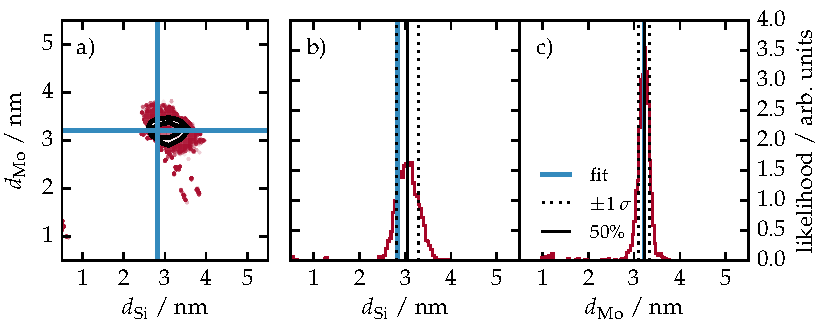
\includegraphics{img/Mo_Si_C_d_Mo_vs_d_Si}
\caption[Results of the maximum likelihood estimation by combination of XRR and EUV reflectivity for the Mo/Si/C samples.]{Results of the maximum likelihood estimation obtained via the \gls{mcmc} procedure similar to Fig.~\ref{ch_spec:fig_ptb17_MCMC_d_Mo_vs_d_Si} but for the combination of \gls{euv} and \gls{xrr} data. a) Two dimensional projection of the likelihood distribution for the parameter pair $d_\text{Si}$ and $d_\text{Mo}$. The projection was obtained by marginalizing over all other parameters of the model. The black contours indicate the areas for one and two standard deviations (corresponding to a coverage factor $k=1$ and $k=2$, respectively). The blue lines in all three sub-figures indicate the best parameter set. b) One dimensional projection of the likelihood distribution for the silicon layer thickness $d_\text{Si}$. The solid black line marks the center position ($50\%$ percentile) of the distribution. The dotted lines are the limits of one standard deviation. c) The one dimensional distribution similarly to b) for the molybdenum layer thickness.}
\label{ch_spec:fig_Mo_Si_C_d_Mo_vs_d_Si}
\end{figure*}
In comparison to the analysis based on only \gls{euv} data for the Mo/B$_4$C/Si/C in Fig.~\ref{ch_spec:fig_ptb17_MCMC_d_Mo_vs_d_Si}, the inclusion of additional \gls{xrr} measurements lead to significantly smaller confidence intervals and thus higher accuracy of the reconstruction. The method of combining the analysis of two datasets of \gls{euv} and \gls{xrr} measurements has been previously applied by others \cite{yakunin_combined_2014}, which have come to the same result of a significantly improved model reconstruction. Each of the methods does provide different sensitivity for the different model parameters. As an example, \gls{euv} measurements are sensitive to the Mo and Si layer thicknesses due to the large optical contrast in that spectral range. On the other hand, high accuracy can be expected from the \gls{xrr} measurements with respect to the period thickness parameter $D$.

In a second step, another \gls{mcmc} optimization was performed on a reduced parameter set, fixing the determined molybdenum layer thickness to its optimal value, i.e.~the $50\%$ percentile of its distribution. Finally, the layer thicknesses of the C barrier layer and the MoSi$_2$ interdiffusion layer were fixed to their nominal values of $d_C = d_{\text{MoSi}_2} = 0.5 $ nm. Due to the broad distribution result for the likelihoods of those parameters, this comes without a limitation of the generality for this analysis, since any value is valid within the predefined boundaries. Additionally, this ensures comparability of the models for all samples without constraining the applicability of the model with respect to the data available.

\begin{figure}[htbp]
\centering
\includegraphics{img/Mo_Si_C_correlation_Si_C}
\caption[Correlation of silicon and carbon layer thickness parameters in the Mo/Si/C model.]{Two-dimensional likelihood distribution indicating the correlation of silicon and carbon layer thickness. The distribution was obtained by marginalizing over all remaining parameters of the model. The blue lines indicate the fit obtained through the two-step \gls{mcmc} optimization procedure (see main text).}
\label{ch_spec:fig_Mo_Si_C_correlation_Si_C}
\end{figure}
The results of the second \gls{mcmc} procedure of the restricted model yield the remaining values for the model parameters by obtaining the globally best solution found. The final result is indicated by the blue solid lines in Fig.~\ref{ch_spec:fig_Mo_Si_C_d_Mo_vs_d_Si}. Due to the choice to restrict the model to a buffer layer thickness of $d_\text{C} = \nm{0.5}$, we find the optimal solution for the silicon layer thickness at the limit of one standard deviation in Fig.~\ref{ch_spec:fig_Mo_Si_C_d_Mo_vs_d_Si}b. The distributions shown represent the \gls{mcmc} results of the unrestricted model, where the silicon and carbon layer thicknesses are strongly correlated as shown in Fig.~\ref{ch_spec:fig_Mo_Si_C_correlation_Si_C}. By fixing the carbon layer thickness to its nominal value, this correlation is resolved and the corresponding silicon layer thickness is well within the interval of one standard deviation as indicated through the solid black contours in Fig.~\ref{ch_spec:fig_Mo_Si_C_correlation_Si_C}.

\subsection{Optimization results} \label{ch_spec:sec_mo_si_c_results}
The theoretical reflectivity curves calculated from the optimal model parameters for the unpolished sample with $d_\text{Mo}^\text{nom} = \nm{3.05}$ are shown in Fig.~\ref{ch_spec:fig_EUV_XRR_combined}. Overall, a very good agreement of the two experiments with the theoretical curves is obtained.
\begin{figure}[htbp]
\centering
\includegraphics{img/PS5657}
\caption[Experimental data in comparison with the theoretical curves for the unpolished Mo/Si/C sample with $d_\text{Mo}^\text{nom} = \nm{3.05}$.]{Experimental data in comparison with the theoretical curves calculated with the model parameters obtained from the combined analysis of \gls{euv} and \gls{xrr} data. The data shown here was measured on the unpolished sample with nominal molybdenum thickness of $d_\text{Mo}^\text{nom} = \nm{3.05}$.}
\label{ch_spec:fig_EUV_XRR_combined}
\end{figure}
The full list for all nominal molybdenum layer thicknesses for all samples with the respective experimental values and their confidence intervals is given in table~\ref{ch_spec:tbl_mo_si_thickness_mcmc_result}.
\begin{table}[htbp]
\centering
\caption[List of nominal molybdenum layer thicknesses in the two Mo/Si/C sample sets.]{List of nominal molybdenum layer thicknesses in the two sample sets. Both sets were fabricated with a equidistant increase in thickness from \nm{1.70} to \nm{3.05} with 9 unpolished and 10 polished samples.}
\label{ch_spec:tbl_mo_si_thickness_mcmc_result}
\begin{tabular}{@{}lll@{}}
\toprule
nom.~$d_\text{Mo}$ / nm & EUV \& XRR &EUV \& XRR\\ 
&(unpolished) & (polished) \\
\midrule
$1.70$ &$1.81({-0.12}/{+0.24})$  &$1.77({-0.22}/{+0.19})$ \\
$1.85$ &$1.98({-0.15}/{+0.14})$  &$1.91({-0.12}/{+0.17})$ \\
$2.00$ &$2.08({-0.11}/{+0.22})$  &$2.29({-0.28}/{+0.13})$ \\
$2.15$ &$2.31({-0.22}/{+0.21})$  &$2.45({-0.43}/{+0.06})$ \\
$2.30$ &$2.43({-0.09}/{+0.16})$   &$2.60({-0.12}/{+0.14})$ \\
$2.45$ &$2.68({-0.13}/{+0.16})$  &$2.58({-0.21}/{+0.15})$ \\
$2.60$ &$2.91({-0.17}/{+0.12})$ &$2.87({-0.22}/{+0.12})$ \\
$2.75$ &$3.02({-0.15}/{+0.15})$  &$3.03({-0.16}/{+0.14})$ \\
$2.90$ &$3.22({-0.13}/{+0.11})$ &$3.15({-0.13}/{+0.13})$ \\
$3.05$ &-  & $3.47({-0.19}/{+0.13})$ \\
 \bottomrule
\end{tabular}
\end{table}

The optimal parameters for the molybdenum layer thickness $d_\text{Mo}$ and the period thickness $D$ found for both sample sets in the two-step \gls{mcmc} analysis are shown in Fig.~\ref{ch_spec:fig_MoSi_fitted_mo_and_fitted_D}.
\begin{figure*}[htbp]
\centering
\includegraphics[width=\textwidth]{img/fitted_mo_and_fitted_D}
\caption[Fitted Mo and period thickness values for both Mo/Si/C sample sets.]{a) Fitted Mo thickness values for both sample sets resulting from the MCMC analysis (see text). The nominal Mo layer thickness is shown in comparison in good agreement with the obtained thicknesses. b) Fitted total period thickness $D$ for both sample sets. For both sample sets, clear jumps can be observed at approx.~$d^\text{nom}_\text{Mo} =2.00$ nm and $d^\text{nom}_\text{Mo} =2.38$ nm, respectively, which is attributed to the crystallization threshold (see text). The marked (circle) samples were measured and analyzed with respect to the diffuse scattering.}
\label{ch_spec:fig_MoSi_fitted_mo_and_fitted_D}
\end{figure*}
The confidence intervals shown in Fig.~\ref{ch_spec:fig_MoSi_fitted_mo_and_fitted_D}a are one standard deviation of the likelihood determined for the Mo layer thickness by the first-step MCMC procedure, i.e.~for the unrestricted model with the parameter limits as listed in table~\ref{ch_spec:tbl_mo_si_c_multilayer_parameters}. The results show the desired linear increase in molybdenum layer thickness, however at a systematically higher thickness than the nominal values. A possible cause for that observation, consistent with the model reconstruction results, is the possible interdiffusion of the molybdenum layer with the silicon and carbon during deposition and a lower molybdenum density. The reduced relative density of the molybdenum layer is indeed found in the reconstruction results for all samples showing systematically reduced density values of $\rho_\text{Mo} \approx 90\%$ w.r.t.~the Mo bulk density. It is reasonable to assume, that the magnetron sputtered Mo layer, which is in mostly amorphous or polycrystalline state, leads to density reduced layers compared to fully crystalline bulk molybdenum. Thus, the nominal amount of deposited molybdenum leads to higher thicknesses than desired. In Fig.~\ref{ch_spec:fig_MoSi_fitted_mo_and_fitted_D}b the fitted period thicknesses $D$ are shown in dependency of the fitted molybdenum thicknesses.

For both sets, distinct jumps can be observed between $d_\text{Mo}\approx\nm{1.9}$ and $d_\text{Mo}\approx\nm{2.3}$ for the polished samples and between $d_\text{Mo}\approx\nm{2.3}$ and $d_\text{Mo}\approx\nm{2.7}$ for the unpolished set. To better understand this observation, Fig.~\ref{ch_spec:fig_EUV_peak_refl} shows the maximum peak reflectance of all \gls{euv} measurements as a function of the reconstructed Mo layer thickness.
\begin{figure}[htbp]
\centering
\includegraphics[width=0.6\textwidth]{img/MoSi_EUV_peak}
\caption[Peak reflectance values for each Mo/Si/C sample in comparison with theoretical expectation.]{Peak reflectance values for each sample obtained from the \gls{euv} measurements for the unpolished sample set (a) and the polished sample set (b). The maximum theoretical reflectance is shown in both subfigures for a perfect (no roughness or interdiffusion) layer system with the same specifications as the samples.}
\label{ch_spec:fig_EUV_peak_refl}
\end{figure}
The identical blue solid line in both subfigures indicates the maximum peak reflectance attainable for a perfect multilayer system with the respective Mo layer thickness without any interdiffusion or roughness. For the calculation, a carbon capping layer of $d_\text{C(cap)} = 2.0$ nm and a relative density of $\rho_\text{C(cap)} = 0.5$ and a silicon dioxide layer of $d_\text{SiO$_2$} = 2.0$ was considered. The dashed curves in both figures show the expected maximum peak reflectance values for the two sample systems calculated by adding the respective roughness/interdiffusion to the model and varying the molybdenum thickness accordingly. In both cases, a significant dip with respect to the expected value can be observed starting at thicknesses of $d_\text{Mo} = 2.31({-0.22}/{+0.21})$ nm for the unpolished samples in Fig.~\ref{ch_spec:fig_EUV_peak_refl}a and at $d_\text{Mo} = 1.77({-0.22}/{+0.19})$ nm for the polished samples in Fig.~\ref{ch_spec:fig_EUV_peak_refl}b. We attribute this significantly diminished peak reflectance to the process of crystallization as the most likely cause. These values are consistent with the increase observed in the period thickness for both cases. Possibly, the deposition is affected by the crystallization threshold causing the increase in period thickness. The values measured here for the dip in peak reflectance are in agreement with earlier observation of molybdenum crystallization in literature \cite{bajt_investigation_2001} for the unpolished sample set. The polishing process shifts that threshold to lower thicknesses by approximately \nm{0.2} to \nm{0.3}.

For a deeper investigation of the interface morphology at the presumed crystallization threshold, \gls{euv} diffuse scattering experiments have been conducted for selected samples of the respective set. To gain a deeper understanding of the reflectivity dip and the period increase, the samples in vicinity of this feature in the Fig.~\ref{ch_spec:fig_EUV_peak_refl} and Fig.~\ref{ch_spec:fig_MoSi_fitted_mo_and_fitted_D} were investigated in comparison to reference samples above and below the threshold. The selection is marked with open circles in Fig.~\ref{ch_spec:fig_MoSi_fitted_mo_and_fitted_D}. This analysis is the topic of chapter~\ref{ch_diff} of this thesis and is described and discussed in detail there based on the model parameters obtained here.

 





\section{Analysis of Cr/Sc Multilayers with Sub-nanometer Layer Thickness} \label{ch_spec:sec_CrSc}
In the previous sections we have characterized multilayer systems designed to reflect radiation in the \gls{euv} spectral range from \nm{12.5} to \nm{14.0} wavelength. There, three to four layer systems per period with period thicknesses of $D\approx\nm{7}$ were used to achieve constructive interference at the desired reflection angles. We shall now apply the analysis to a different system, multilayer mirrors designed to reflect radiation in the spectral range between \nm{2.2} and \nm{4.4} wavelength, the so called \emph{water window}. Those systems share the basic principle of a one-dimensional Bragg crystal with the Mo/Si multilayer stacks from the previous sections, but differ in the selection of materials and their layer thicknesses. The intrinsic relationship between spectral range and period thickness to achieve constructive interference, requires period thicknesses of $D\approx \nm{1.5}$ for this case and higher number of period replications.


The system we investigate here is a bilayer stack of chromium (Cr) and scandium (Sc). A detailed description of the sample preparation process and the choice of the layer materials can be found in Ch.~\ref{ch_exp}, Sec.~\ref{ch_exp:sec_multilayer_design}. The sample is optimized to reflect radiation of $\lambda = \nm{3.14}$ at an angle of incidence of $\alpha_i = \SI{1.5}{\degree}$. It has $N=400$ bilayer periods, where the last period has a larger Cr capping layer thickness. The model of the sample is shown in Fig.~\ref{ch_spec:fig_Cr_Sc_model}.
\begin{figure}[htbp]
    \def\svgwidth{0.7\textwidth}
    \fontfamily{fds}\selectfont\footnotesize
    \import{svg/}{cr_sc_model.pdf_tex}
    \caption[Model of the Cr/Sc multilayer stack including the substrate and the capping layers.]{Model of the Cr/Sc multilayer stack including the substrate and the capping layers. The periodic part is enclosed between the dashed lines with two layers in each period repeated $N=400$ times. The capping period does include the thicker chromium layer deposited to avoid oxidation of the periodic stack. Furthermore, oxide and carbon contamination layers are considered at the top surface.}
    \label{ch_spec:fig_Cr_Sc_model}
\end{figure}
The small period thickness of only $D\approx\nm{1.5}$ for this type of sample yields individual layer thicknesses in the sub-nanometer regime, for a bilayer period with approximately equal individual layer thicknesses. This is a significant difference to the Mo/Si systems treated in the beginning of this chapter, where the molybdenum and silicon layers were well above $>\nm{1.7}$. The exception in the previous case were the buffer and interdiffusion layers, which nominally have thicknesses below one nanometer and could not be characterized based on the methods employed above. In the Cr/Sc system investigated here, all nominal layer thicknesses are in that order of magnitude and are thus challenging to characterize. We shall therefore first compare the results obtained with an approach similar to the methods in the previous sections to establish a limit to the applicability of discrete layer models.

\subsection{Reconstruction with a discrete layer model approach} \label{ch_spec:sec_CrSc_resconstrution_binary}
In analogy to Sec.~\ref{ch_spec:sec_mo_si_c}, we seek to reconstruct the individual layer thicknesses based on experimental data. For this we construct a discrete layer model as illustrated in Fig.~\ref{ch_spec:fig_Cr_Sc_model} in analogy to the procedure applied for the Mo/Si multilayer systems. The parameters of this discrete layer model are listed in table~\ref{ch_spec:tbl_cr_sc_binary_parameters} together with the upper and lower bound for the particle swarm optimization procedure.
\begin{table*}[htbp]
\centering
\caption{Parametrization of the Cr/Sc binary multilayer model.}
\label{ch_spec:tbl_cr_sc_binary_parameters}
\begin{tabular}{@{}llll@{}}
\toprule
Parameter & Definition & Lower bound & Upper bound\\ \midrule
$d_\text{Cr}$ / nm & Cr layer thickness & $0.0$& $1.5$\\ 
$d_\text{Sc}$ / nm & Sc layer thickness& $0.0$& $1.5$\\ 
$\sigma$ / nm & N\'{e}vot-Croce parameter& $0.0$& $0.5$\\ 
&(identical for all interfaces)&&\\
$\rho_\text{Cr}$ &Cr density w.r.t.~bulk density & $0.5$& $1.0$\\ 
$\rho_\text{SC}$ &Sc density w.r.t.~bulk density& $0.5$& $1.0$\\ 
\midrule
\multicolumn{4}{c}{Capping layer}\\
\midrule
$d_\text{C (cap)}$ / nm & C capping layer thickness & $0.0$&$1.0$ \\ 
$d_\text{CrO (cap)}$ / nm & SiO$_2$ capping layer thickness & $0.0$&$1.5$ \\ 
$d_\text{Cr (cap)}$ / nm & SiO$_2$ capping layer thickness & $0.0$&$3.0$ \\ 
$\rho_\text{C (cap)}$ &C density w.r.t.~bulk density& $0.0$& $1.0$\\ 
$\rho_\text{CrO (cap)}$& CrO density w.r.t.~bulk density& $0.0$& $1.0$\\
$\rho_\text{Cr (cap)}$& Cr (cap) density w.r.t.~bulk density & $0.5$& $1.0$  \\
 \bottomrule
\end{tabular}
\end{table*}

The reflectivity of the sample in the water window spectral range from \nm{3.12} to \nm{3.16} was measured at the \gls{sx700} beamline at \gls{bessy}. The angle of incidence was $\alpha_i=\SI{1.5}{\degree}$ (corresponding to a grazing angle of incidence of $\alpha_i^\text{GI} = \SI{88.5}{\degree}$), which corresponds to the design goal for this mirror prototype. In addition, similar to the Mo/Si samples, a \gls{xrr} measurement was 
conducted in the group of Sa\v{s}a Bajt at the DESY laboratory using a laboratory-based X-ray diffractometer 
(X'Pert PRO MRD, Panalytical). The diffractometer is equipped with a high-resolution goniometer and uses Cu-K$_\alpha$ radiation as a source. The \gls{xrr} intensities were recorded using a PIXcel counting detector. The dynamic range achieved in the measurements 
extended down to a reflectance of $10^{-6}$ for grazing angles of incidence of 
$\alpha_i=0^\circ$ to $\alpha_i=3^\circ$.

Both measurement curves are shown together in Fig.~\ref{ch_spec:fig_CrSc_EUV_XRR_data}.
\begin{figure}[htbp]
  \centering
  \includegraphics[width=0.6\textwidth]{img/CrSc_EUV_XRR_data}
  \caption[EUV and XRR data recorded for the Cr/Sc sample system.]{\Gls{euv} and \gls{xrr} data recorded for the Cr/Sc sample system. a) The \gls{euv} curve was obtained at an angle of incidence $\alpha_i=\SI{1.5}{\degree}$. b) The \gls{xrr} curve was recorded using a Cu-K$_\alpha$ source with a photon energy of $E_\text{ph}=\ev{8048}$.}
  \label{ch_spec:fig_CrSc_EUV_XRR_data}
\end{figure}
Due to the short period of the multilayer sample, only two Bragg peaks could be observed in this angular range in the \gls{xrr} curve. All expected higher order peaks were below the detection threshold of $10^{-6}$ in reflected intensity. The dominating experimental uncertainty was the inhomogeneity of the sample stack across the sample area. The given uncertainty values for each of the measurement points were estimated, by measuring the peak reflectance of the \gls{euv} reflectivity curve on positions marking a cross of \mm{2} by \mm{2} in the sample center. This data was compared to theoretical expectance value based on a \gls{pso} fit of the discrete layer model above (for details of the optimization results see below). From this a drift of the period thickness of $D=\SI{2}{\pico\meter}$ was obtained and uncertainties were calculated as the difference of two theoretical curves attaining the maximum and minimum $D$ values. Similarly, uncertainties for the \gls{xrr} curve were calculated by simulating theoretical curves based on the same period drifts.

In comparison, the most remarkable difference with respect to the Mo/Si mirrors is the significantly reduced measured peak reflectance of the \gls{euv} curve in Fig.~\ref{ch_spec:fig_CrSc_EUV_XRR_data}a compared to the curves in Fig.~\ref{ch_spec:fig_ptb17_reflectance_AOI_15} and Fig.~\ref{ch_spec:fig_EUV_peak_refl}. The maximum experimental value attained is only approximately $R_\text{max} \approx 15\%$ while it is up to $R_\text{max} \approx \SI{70}{\percent}$ for the Mo/Si systems.

To better illustrate the differences to the Mo/Si systems, we have conducted an 
analysis based on the discrete layer model of a Cr/Sc multilayer as described above. The particle swarm optimization was done based on the EUV data shown in Fig.~\ref{ch_spec:fig_CrSc_EUV_XRR_data}a and the parameters and limits listed in table~\ref{ch_spec:tbl_cr_sc_binary_parameters}. The resulting parameters are listed in table~\ref{ch_spec:tbl_cr_sc_binary_pso_results}.
\begin{table}[htbp]
\centering
\caption{\gls{pso} fit results for the discrete layer Cr/Sc multilayer model.}
\label{ch_spec:tbl_cr_sc_binary_pso_results}
\begin{tabular}{@{}ll@{}}
\toprule
Parameter &  \gls{pso} result\\ \midrule
$d_\text{Cr}$ / nm &  $0.8224$\\ 
$d_\text{Sc}$ / nm &  $0.7510$\\ 
$\sigma$ / nm &  $0.375$\\ 
$\rho_\text{Cr}$  & $0.876$\\ 
$\rho_\text{Sc}$ & $0.957$\\ 
\midrule
\multicolumn{2}{c}{Capping layer}\\
\midrule
$d_\text{C (cap)}$ / nm  & $0.462$ \\ 
$d_\text{CrO (cap)}$ / nm  & $1.143$ \\ 
$d_\text{Cr (cap)}$ / nm  & $2.322$ \\ 
$\rho_\text{C (cap)}$ & $0.502$\\ 
$\rho_\text{CrO (cap)}$& $0.618$\\
$\rho_\text{Cr (cap)}$ & $0.851$\\
 \bottomrule
\end{tabular}
\end{table}
The capping layer results were obtained in a combined \gls{pso} analysis based on the \gls{euv} and \gls{xrr} data excluding the areas of the Bragg peaks. This grazing incidence reflectivity data has a very high sensitivity for the top surface layers, which can not be deducted from an \gls{euv} curve alone as demonstrated in Sec.~\ref{ch_spec:sec_reconstruction_PTB17}.

The theoretical curve obtained from the \gls{pso} procedure is shown in Fig.~\ref{ch_spec:fig_CrSc_binary_fit_vs_max_refl} in direct comparison with the theoretically achievable maximum reflectivity curve.
\begin{figure}[htbp]
  \centering
  \includegraphics[width=0.45\textwidth]{img/CrSc_binary_fit_vs_max_refl}
  \caption[Fitted experimental EUV reflectance curves for the Cr/Sc sample.]{Fitted experimental EUV reflectance curves across the wavelength 
of the radiation impinging at $\alpha_i=1.5^\circ$ from normal, based on the binary 
model. The green curve shows the maximum theoretical reflectance assuming a perfect multilayer system without roughness or interdiffusion.}
  \label{ch_spec:fig_CrSc_binary_fit_vs_max_refl}
\end{figure}
The latter was obtained by calculating the resulting reflectivity based on the parameter results in table~\ref{ch_spec:tbl_cr_sc_binary_pso_results}, but without any roughness or interdiffusion, i.e.~by requiring $\sigma \equiv 0.0$. The Sc 
to Cr ratio was found to be $\Gamma_\text{Sc}= d_\text{Sc}/d_\text{Cr} = 0.48$ with a \gls{rms} value of $\sigma=0.385$ nm for the N\'{e}vot-Croce factor. While the EUV reflectance curve shows excellent agreement with the measured data, there is a significant offset to the theoretically achievable maximum reflectance. For the particular model derived above, theoretical reflectance values of $R_\text{max} > \SI{50}{\percent}$ are possible. This large difference, especially compared to Mo/Si systems which are very close to the theoretically achievable maximum reflectance (cf.~Fig.~\ref{ch_spec:fig_EUV_peak_refl}), hints at strong roughness or intermixing of the two materials. To verify the applicability of the discrete (binary) layer model used here, the calculated curves for both experiments, the \gls{euv} and \gls{xrr} curve, are shown together in Fig.~\ref{ch_spec:fig_CrSc_binary_model_EUV_vs_XRR}.
\begin{figure*}[htbp]
  \centering
  \includegraphics[width=\textwidth]{img/CrSc_binary_model_EUV_vs_XRR}
  \caption[Comparison of EUV and XRR fitting results for the binary Cr/Sc model approach.]{a) Measured \gls{euv} reflectivity curve for the near-normal angle of incidence of $\alpha_i=\SI{1.5}{\degree}$ together with the theoretical curve based on the \gls{pso} optimized binary multilayer model. b) Measured and calculated \gls{xrr} curves for the same sample and model parameters at grazing angles of incidence using radiation at the Cu-K$_\alpha$ wavelength. A clear mismatch of the theoretical curve and the measured data can be observed for the second Bragg peak between $\alpha_i^\text{GI} = \SI{5.0}{\degree}$ and $\alpha_i^\text{GI} = \SI{6.0}{\degree}$.}
  \label{ch_spec:fig_CrSc_binary_model_EUV_vs_XRR}
\end{figure*}

Again, the \gls{euv} data is matched rather good, while in the case of the \gls{xrr} measurement only the first Bragg peak is found to be matched by the model also in the X-ray regime. However, the second Bragg resonance, clearly visible with a peak reflectance value of approximately $10^{-3}$ is not represented by the model at all. A fully
combined analysis similarly to the approach in Sec.~\ref{ch_spec:sec_mo_si_c} did not yield a consistent result. The \gls{rms} value for $\sigma$ required to reduce the theoretical EUV reflectance down to the measured 
level could not be brought into agreement with the existence of the second Bragg peak in the \gls{xrr} curve. In a strictly binary model like this one with a layer thickness ratio of 
$\Gamma_\text{Sc}\approx 0.5$, the second Bragg peak is additionally suppressed 
due to symmetry reasons. Thus, there is a clear mismatch of the model reconstruction and the experimental observations, mostly due to the complementary data delivered through the measurement of the second Bragg peak of the \gls{xrr} curve. This is a strong indicator, that the simple model as defined above does not suffice to describe the sample. Therefore, a more elaborate model is required introducing additional parameters to account for the increased complexity of the samples layer properties compared to the Mo/Si sample systems above.

\subsection{Extending The Model to Graded Interfaces and Interdiffusion} \label{ch_spec:sec_CrSc_gradual_model}
The physical structure of Cr/Sc multilayer systems with individual layer thicknesses in the sub-nanometer regime is significantly different than in case of the comparably large thicknesses of several nanometers in the Mo/Si case of the two preceding sections. It is well known \cite{prasciolu_thermal_2014}, that magnetron sputtered Cr and Sc multilayer systems, similarly to the Mo/Si systems, suffer from imperfect interfaces. Phase diagrams of Cr/Sc systems show, that the two materials do not like to mix or form composites at the interfaces \cite{boer_cohesion_1988}. That makes them an ideal candidate for chemically abrupt multilayer structures as needed for multilayer mirrors. However, due to the very thin layer structure, both materials are in an amorphous state and intermixing was in fact observed for multilayer structures similar to the one discussed here \cite{ghafoor_incorporation_2008}. Another possible reason is the magnetron sputtering deposition, which has shown to cause intermixing upon deposition \cite{eriksson_enhanced_2002}. In addition, roughness at the interfaces exists and further diminishes an ideal chemically abrupt transition from one material to the next. Due to the small layer thicknesses required to achieve the first Bragg resonance upon near-normal incidence with radiation of $\lambda=\nm{3.14}$, roughness and interdiffusion may occur over a zone as large as the total layer thickness itself. The results from the specular \gls{euv} and \gls{xrr} measurements shown above, clearly demonstrate that a binary model with only a N\'{e}vot-Croce damping parameter $\sigma$ does not provide an accurate model for the physical structure. Instead, a more complex model is required. Here, we define a periodic model to account for possible interdiffusion gradients and intermixing between the two materials in the stack. The symmetry of two identically thick layers within one period in the simple model above leads to a suppression of the second order Bragg peak. Nevertheless, physically this symmetry effect can be broken by interdiffusion zones with different thicknesses, depending on whether Cr was deposited on Sc or vice versa. Thereby, the second Bragg peak is no longer suppressed even though both layers have the same thickness if the interdiffusion zones are asymmetric. The model, which we use to reconstruct the Cr/Sc multilayer sample measured above is illustrated in Fig.~\ref{ch_spec:fig_CrScModel} in direct comparison to the simple model used before.
\begin{figure*}[htb]
    \def\svgwidth{\textwidth}
    \import{svg/}{CrSc_model.pdf_tex}
    \caption[Binary and gradual Cr/Sc multilayer models.]{a) Binary Cr/Sc multilayer model with total period thickness $D$ and 
the individual layer thicknesses $d_\text{Sc}$ and $d_\text{Cr}$. b) Model with 
explicit gradual interfaces following a sinusoidal profile. The ideal interface 
profile is approximated through discrete sublayers as indicated in red, forming 
the actual gradual interface profile entering the electric field calculations. 
The thickness of the interdiffusion zones can differ for the top and bottom 
interface in each period. Their total thicknesses are given by $s_\text{Sc}$ 
and $s_\text{Cr}$. The effective index of refraction for both layers is given 
by $\tilde{n}_\text{Sc}$ and $\tilde{n}_\text{Cr}$, respectively.}
    \label{ch_spec:fig_CrScModel}
\end{figure*}
The interdiffusion zones are modeled following a sinusoidal profile, which represents a smooth transition from the refractive index of the Cr layer to the Sc layer and vice versa. The thickness of those zones is given by the parameters $s_\text{Sc}$ and $s_\text{Cr}$. For the calculation of the electromagnetic fields inside the stack, the interface region is sampled with a fixed number of equally spaced points in $z$-direction, effectively creating a region of thin sublayers with a gradually changing index of refraction (illustrated by the red stepped function in Fig.~\ref{ch_spec:fig_CrScModel}). To take into account intermixing extending across the full period, we introduced an intermixing parameter $\eta$. The effective indices of refraction of the individual Cr and Sc layers are then given through
\begin{align}
\tilde{n}_\text{Cr} &=(\eta/2) n_\text{Sc} + (1-\eta/2) n_\text{Cr} \text{,} 
\nonumber\\
\tilde{n}_\text{Sc} &=(1-\eta/2) n_\text{Sc} + (\eta/2) n_\text{Cr} \text{,} 
\label{eqn:effective_n} \\
&\text{for} \quad \eta \in [0,1] \text{,}\nonumber
\end{align}
where $n_\text{Cr}$ and $n_\text{Sc}$ are the tabulated values \cite{henke_x-ray_1993} 
with densities $\rho_\text{Cr}$ and $\rho_\text{Sc}$. Similarly as discussed in the case of the Mo/Si multilayer systems, the densities serve to consider unknown uncertainties in the tabulated values of the optical constants with respect to the actual case in the samples.

With the definition of the model as outlined above, natural restrictions arise for the parameters. As an example, the interdiffusion zone region can not extend across half of the thickness of the original layers total thickness described by the parameter $d_\text{Cr}$ or $d_\text{Sc}$, respectively. Instead, the intermixing parameter would have to be increased to account for that situation. The model is therefore parametrized according to the list of effective parameters given in table~\ref{ch_spec:tbl_CrSc_gradual_parametrization} together with their allowed ranges for the optimization procedure in analogy to the analysis conducted in the previous sections. The range limits arise either from physical plausibility or are intrinsic properties of the parameter definition.
\begin{table*}[htbp]
\centering
\caption{Multilayer parametrization and parameter limits}
\label{ch_spec:tbl_CrSc_gradual_parametrization}
\begin{tabular}{@{}llll@{}}
\toprule
Parameter & Definition & Lower bound & Upper bound\\ \midrule
$D$ / nm & $= d_\text{Sc} + d_\text{Cr}$ & 1.5&1.6 \\ 
$\Gamma_{Sc}$ & $= d_\text{Sc} / D$&0.0 &1.0 \\ 
$s_d$ / nm&$=s_\text{Sc} + s_\text{Cr}$&0.0 & 1.6\\ 
$\Gamma_s$ &$= s_\text{Sc} / s_d$& 0.0& 1.0\\ 
$\eta$ &layer intermixing& 0.0& 1.0\\ 
$\sigma_r$ / nm & r.m.s.~roughness& 0.0& 0.5\\ 
$\rho_{Sc}$ &Sc density w.r.t.~bulk density & 0.5& 1.0\\ 
$\rho_{Cr}$ &Cr density w.r.t.~bulk density& 0.5& 1.0\\ 
 \bottomrule
\end{tabular}
\end{table*}
Here, $D$ is the full period thickness, $d_\text{Sc}$ and $d_\text{Cr}$ are the 
nominal layer thicknesses of the Cr and Sc layers as indicated in 
Fig.~\ref{ch_spec:fig_CrScModel}, and $\rho_\text{Sc}$ and $\rho_\text{Cr}$ their 
respective densities with respect to their bulk densities 
$\tilde{\rho_\text{Sc}} = 2.989$ g/cm$^3$ and $\tilde{\rho_\text{Cr}} = 7.19$ 
g/cm$^3$ \cite{henke_x-ray_1993}. The loss of specular 
reflectance due to roughness-induced scattering is considered through the 
N\'{e}vot-Croce factor using $\sigma_\text{r}$ identical at each interface. This is necessary to account for diffusely scattered light, which is missing in the measured specularly reflected radiation but can not be attributed to contrast loss due to interdiffusion. The parameter $\Gamma_\text{Sc}$ indicates the portion of the Sc layer thickness 
with respect to the full period thickness $D$, which together uniquely define the thickness $d_\text{Cr}$; $\Gamma_\sigma$ describes the 
asymmetry of the widths of the interdiffusion zones at the Cr on Sc and Sc on Cr 
interfaces and is intrinsically limited to the interval $\Gamma_\sigma \in [0,1]$. Note that 
$s_\text{Sc}$ and $s_\text{Cr}$ are half periods of the sinus functions used to 
describe the interface profiles. Therefore the condition $s_\text{Sc} + 
s_\text{Cr} \leq D$ holds.

The discretization of the smooth interface profile in the interdiffusion zones introduces an additional numerical uncertainty through the number of discretization points $n$ required to reflect the physical situation of a smooth transition. To assert a lower limit for this number, we have evaluated the mean error introduced by coarse sampling. The most accurate experiment of the analysis within this chapter is given by the \gls{euv} reflectivity curve, which serves as a reference for this assertion through the sum of the squared uncertainty of each data point in Fig.~\ref{ch_spec:fig_CrSc_EUV_XRR_data}a, $\sum_m \tilde{\sigma}_m$. 

The numerical error of the model depending on the interface sampling through gradual sublayers was evaluated by comparing the sum of squares
\begin{align}
\chi_n &= \sum\limits_m (I^{n=100}_m - I^n_m)^2
\end{align}
of the difference of the theoretical \gls{euv} curves with increasing numbers of gradual interfaces and an ``ideal'' smooth transition represented by $100$ sublayers. The model parameters used for this analysis were obtained through a \gls{pso} optimization of the model with respect to the \gls{euv} reflectivity curve.
\begin{figure}[htbp]
  \centering
  \includegraphics[width=0.45\textwidth]{img/CrSc_numerical_uncertainty_mixlayer}
  \caption{Numerical uncertainty introduced through a coarse graded Cr/Sc layer model in comparison with the experimental uncertainty.}
  \label{ch_spec:fig_CrSc_numerical_uncertainty_mixlayer}
\end{figure}
As illustrated in Fig.~\ref{ch_spec:fig_CrSc_numerical_uncertainty_mixlayer}, the experimental uncertainty dominates at the lower limit of $n=10$ sublayers for the interface zone.
For the analysis is this chapter, and due to reasons of numerical effort required to calculate the electromagnetic field for all measurements discussed here, we use $n=15$ sublayers for all calculations. At that value, the experimental uncertainty is clearly dominant and only a marginal additional numerical error is acquired due to insufficient sampling.

As a verification of the applicability of the model to the problem of accurately representing the physical structure that could describe the \gls{euv} and \gls{xrr} data shown in Fig.~\ref{ch_spec:fig_CrSc_EUV_XRR_data} above, the combined analysis technique has been applied to the two data sets described in Sec.~\ref{ch_spec:sec_MoSi_euv_xrr_combined} based on the improved gradual model. The particle swarm optimization approach is used to obtain a global solution for the model parameters by minimizing the functional defined in Eq.~\eqref{ch_spec:eqn_Mo_Si_C_total_chi_2}. The results found for the gradual model are shown in Fig.~\ref{ch_spec:fig_CrSc_bianry_vs_gradual_model_fits}.
\begin{figure*}[htbp]
  \centering
  \includegraphics[width=\textwidth]{img/CrSc_bianry_vs_gradual_model_fits}
  \caption{Measaured and calculated curves based on the reconstruction results for the gradual model and the \gls{euv} and \gls{xrr} data. a) Measured \gls{euv} reflectivity curve for and near-normal angle of incidence of $\alpha_i=\SI{1.5}{\degree}$ together with calculated curve of the \gls{pso}-based gradual model reconstruction. b) Measured and calculated \gls{xrr} curves for the same sample and model parameters at grazing angles of incidence using radiation at the Cu-K$_\alpha$ wavelength.}
  \label{ch_spec:fig_CrSc_bianry_vs_gradual_model_fits}
\end{figure*}
The \gls{euv} reflectivity curves show visually indistinguishable fits for both, the binary model shown in Fig.~\ref{ch_spec:fig_CrSc_binary_model_EUV_vs_XRR} and the gradual model in Fig.~\ref{ch_spec:fig_CrSc_bianry_vs_gradual_model_fits}a. For the binary model, we have seen the distinct mismatch with the second order Bragg peak. For the gradual interface model, we see a significant improvement of the optimized result with a perfect match in both Bragg peaks of the \gls{xrr} curve in Fig.~\ref{ch_spec:fig_CrSc_bianry_vs_gradual_model_fits}d while also maintaining an excellent agreement with the \gls{euv} curve.

Based on the example of a combined analysis of \gls{euv} and \gls{xrr} data in this section, the gradual interface model clearly provides a more accurate representation of the sample than the binary approach by offering a reconstruction satisfying both data sets. At the same time, the results show that a verification of the model only becomes possible by adding complementary information. In case of the example above, that information is provided through the appearance of a second Bragg peak in the \gls{xrr} curve. Thereby, the limiting case of the binary model, which is still possible for the new gradual model, can be excluded with certainty through the comparison shown in Fig.~\ref{ch_spec:fig_CrSc_bianry_vs_gradual_model_fits}. The main difference of both models is the local gradual change of the index of refraction, which attributes for the fact that both materials may intermix. More importantly, both materials may intermix differently with respect to the specific interface, i.e.~the situation where Cr is deposited on top of Sc or vice versa. A key element of obtaining a reconstruction of that particular model is thus the application of experimental techniques, which can deliver information on the spacial distribution of the materials within one period.

At that point, it should be noted that other distortions of a perfect layer system can be imagined, which are not covered by a strictly periodic model as the one introduced above. Those include drifts of the period thickness $D$ across the stack or other systematic aperiodicities. In that case, however, a broadening of the peak or a distortion of the peaks symmetry, most prominently in the \gls{euv} curve, will be observed, which is not the case (for example, cf.~Fig.~\ref{ch_spec:fig_CrSc_drift} below). Although situations may occur, where the aperiodicities could lead to effects compensated by tuning the parameters of the gradual interface model, this assumption would assume a more complex situation than the simple assumption of periodicity and thus lead to a more complex, ill-defined model which could not be reconstructed.
To further strengthen that argument, we shall calculate the distortion occurring through a drift in the deposition process. This is a plausible systematic error, which could be caused by instabilities in the deposition process. Fig.~\ref{ch_spec:fig_CrSc_drift} shows the peak distortion for a drift of the total period thickness $D$ across the whole stack of $N=400$ periods by $d_\text{drift} = \nm{0.005}$ based on the model parameters for the curves in Fig.~\ref{ch_spec:fig_CrSc_bianry_vs_gradual_model_fits}c keeping the mean period thickness constant. Clearly, already this drift would cause a distortion of the peak symmetry with a significant minimum at $\lambda \approx \nm{3.136}$ and an additional shoulder at $\lambda \approx \nm{3.153}$, which is not observed in the data.
\begin{figure}[htbp]
  \centering
  \includegraphics{img/CrSc_drift}
  \caption[EUV peak deformation assuming a constant drift in the Cr/Sc period thickness.]{\Gls{euv} peak deformation assuming a constant drift of $d_\text{drift} = \nm{0.005}$ across the total multilayer stack keeping the mean period thickness $D$ constant.}
  \label{ch_spec:fig_CrSc_drift}
\end{figure}

\subsection{Addition of Complementary Experimental Methods}
Due to the increased complexity of the model, the question arises how accurately any parameter of the model can be determined and whether correlations exist and can be resolved (cf.~Fig.~\ref{ch_spec:fig_Mo_Si_C_correlation_Si_C} as an example for correlated model parameters in case of Mo/Si multilayer systems) based on the available data and whether further analytical measurements can improve the result as this was clearly the result for the combination of \gls{euv} and \gls{xrr} experiments shown above. For the particular case of the gradual interface model for periodic multilayer systems with sub-nanometer layer thicknesses, in total four experiments were conducted to study the applicability of each method with respect to finding a unequivocal reconstruction including confidence intervals. Only by systematically analyzing the strength and weaknesses of the employed analytic methods, a reconstruction of the model resembling the reality inside the sample becomes possible.

\subsubsection{Resonant EUV Reflectivity}
As seen for the four layer system discussed in Sec.~\ref{ch_spec:sec_reconstruction_PTB17}, confidence intervals for the individual layer thicknesses in the range below \nm{1} could not be obtained by exclusively analyzing the \gls{euv} curve. Similarly, the combined analysis of \gls{euv} and \gls{xrr} experiments in Sec.~\ref{ch_spec:sec_MoSi_euv_xrr_combined} did improve the result but still shows fairly large confidence intervals concerning the small total layer thickness in the Cr/Sc systems. For the particular system discussed here with possibly strong interdiffusion, a technique is required that yields the total amount of Sc and equivalently Cr within a single period. For that purpose, resonant reflectivity experiments in the \gls{euv} spectral range are promising. The knowledge of the optical constants are a necessary requirement for deducting quantitative information from that kind of experiment. In case of Sc, those were measured precisely for the Sc L3 and L2 absorption edges at approximately $\lambda_\text{Sc-L} \approx \nm{3.1}$ and below by \textcite{aquila_measurements_2004}. The real and imaginary parts obtained from that experiments are shown together with the respective optical constants of Cr in Fig.~\ref{ch_exp:fig_crsc_contrast} of Sec.~\ref{ch_exp:sec_multilayer_design}. To exploit the information contained in the optical constants of Sc, angular resolved reflectivity curves across the first Bragg peak were recorded at several wavelengths across the Sc L-edge. As the Cr dispersion is changing only marginally and smoothly across that wavelength range, any change of contrast and absorption can be attributed to the Sc in the multilayer. The corresponding measurements are shown in Fig.~\ref{ch_spec:fig_CrSc_REUV_data}.
\begin{figure}[htbp]
  \centering
  \includegraphics[width=0.7\textwidth]{img/CrSc_REUV_data}
  \caption[Measured resonant EUV reflectivity curves across the Sc L2 and L3-edge in logarithmic representation.]{Measured resonant \gls{euv} reflectivity curves across the Sc L2 and L3-edge in logarithmic representation. At each equidistant photon energy point, an angular resolved reflectivity curve was recorded across the Bragg peak.}
  \label{ch_spec:fig_CrSc_REUV_data}
\end{figure}
Each reflectivity curve was recorded within the interval from $\alpha_i = \SI{2.5}{\degree}$ to $\alpha_i = \SI{19.0}{\degree}$, with varying upper and lower boundary depending on the selected wavelength to incorporate only the range of the Bragg peak. The wavelength range was chosen between $\lambda = \nm{2.986}$ and $\lambda = \nm{3.128}$ including the Sc L2 and L3 edges. The resulting data is analyzed in analogy to the \gls{euv} reflectivity curves in Sec.~\ref{ch_spec:sec_CrSc_gradual_model} by applying the matrix algorithm on basis of the gradual layer model and the optical constants by \textcite{aquila_measurements_2004}. The experimental uncertainties taken into account for the \gls{reuv} experiment were estimated on basis of the multilayer inhomogeneity deducted as described for the \gls{euv} experiment in Sec.~\ref{ch_spec:sec_CrSc_resconstrution_binary}. It should be noted, that uncertainties for the measured optical constants were not given by the authors of the respective publication. Nevertheless, again by allowing a variation of the densities of the respective materials in the model, those are accounted for in the analysis. The variation, however, uses the same value for this density parameter for all analyzed curves. A missmatch of the individual reflectivity curves at the different energies with the theoretical calculation based on the results by Aquila~et~al.~is thus possible. This leads to a broadening of the likelihood distribtution, and thereby an increase of the confidence intervals reflecting the uncertainty in the optical constants determination. The details of the reconstruction based on this dataset are shown below in this section.

\subsubsection{Grazing Incidence X-ray Fluorescence}
In addition to the reconstruction of the Sc content via the \gls{reuv} experiment, spacial resolved measurements are necessary to deduct the interface profile in the gradual layer model. As discussed in Sec.~\ref{ch_spec:sec_CrSc_gradual_model}, asymmetric interface regions provide a possibility to observe a second Bragg peak in the \gls{xrr} measurement, even though both layers in the period have equal nominal thickness. To obtain information on that spacial distribution of both materials within a period, \gls{xrf} experiments exploiting the formation of a standing wave when scanning across the first Bragg peak were performed. The details of the method and how spacial sensitivity can be obtained are described in detail in Ch.~\ref{ch_theo}, Sec.~\ref{ch_theo:sec_xrf}.

The sample was measured exciting fluorescence of the Sc and Cr K-lines, which show the highest fluorescence yield for the core shell transitions. The K-edges for both materials are at energies of $E_\text{Sc-K} = \ev{4492}$ and $E_\text{Cr-K} = \ev{5989}$ \cite{elam_new_2002}. The experiment was therefore conducted at the \gls{fcm} beamline at \gls{bessy} in grazing incidence geometry at photon energies of $E_\text{ph} = \ev{5500}$ and $E_\text{ph} = \ev{6250}$, well above the respective edges as described in Ch.~\ref{ch_exp}, Sec.~\ref{ch_exp:sec_xrf_at_fcm}. Depending on which energy was used, the Bragg peak is found at grazing angles of incidence of $\alpha_i^\text{GI} \approx \SI{4.12}{\degree}$ and $\alpha_i^\text{GI} \approx \SI{3.62}{\degree}$, respectively. The measured relative fluorescence yield in the vicinity of the first Bragg peak is shown in Fig.~\ref{ch_spec:fig_CrSc_fluorescence_data} for both photon energies and materials. Here, due to the grazing angles of incidence, the method is referred to as \gls{gixrf}.
\begin{figure*}[htbp]
  \centering
  \includegraphics[width=\textwidth]{img/CrSc_fluorescence_data}
  \caption[Measured relative X-ray fluorescence curves for the Cr and Sc K-lines across the first Bragg peak of the Cr/Sc sample.]{Measured relative X-ray fluorescence curves for the Cr and Sc K-lines across the first Bragg peak. a) Relative fluorescence yield of the Sc K-line at a primary photon energy of $E_\text{ph}=\ev{5500}$. b), c) Relative fluorescence yield for both materials at an primary photon energy of $E_\text{ph} = \ev{6250}$.}
  \label{ch_spec:fig_CrSc_fluorescence_data}
\end{figure*}
Since the photon energy of $E_\text{ph} = \ev{5500}$ is below the K-edge of Cr, only data for the Sc K-fluorescence exists. In the second case, fluorescence from both materials was detected. The measurement uncertainties were estimated from the scattering of the data for regions away from the Bragg resonance, where a flat curve is theoretically expected.

The fluorescence curves for Cr and Sc show distinctly different behavior and the expected curve shape (cf.~Fig.~\ref{ch_theo:fig_xrf_scheme}). For the analysis, the result at photon energies of $E_\text{ph}=\ev{5500}$ (Fig.~\ref{ch_spec:fig_CrSc_fluorescence_data}a)  was not taken into account, as the information is redundant to the result at  $E_\text{ph}=\ev{6250}$ (Fig.~\ref{ch_spec:fig_CrSc_fluorescence_data}b). As mentioned above, the theoretical description on how the relative fluorescence is calculated based on the gradual model is elaborated on in detail in Ch.~\ref{ch_exp}, Sec.~\ref{ch_exp:sec_xrf_at_fcm}.

\subsection{Reconstruction and Maximum Likelihood Evaluation}\label{ch_spec:sec_CrSc_results}
With the two additional measurements described above, five data sets (\gls{euv}, \gls{xrr}, \gls{reuv}, \gls{gixrf} (Sc) and \gls{gixrf} (Cr)) are available for the Cr/Sc multilayer sample to reconstruct the parameters of the gradual interface model. The full dataset, repeating and summarizing the relevant experimental results of this section in one figure, is compiled in Fig.~\ref{ch_spec:fig_CrSc_all_data}.
\begin{figure*}[htbp]
  \centering
  \includegraphics[width=\textwidth]{img/CrSc_all_data}
  \caption[Full data set from the Cr/Sc sample used in the combined analysis.]{Full data set used in the combined analysis. Due to redundancy, the \gls{xrf} data for the Sc at a photon energy of $E_\text{ph}=\ev{5500}$ was omitted.}
  \label{ch_spec:fig_CrSc_all_data}
\end{figure*}

As in the combined analysis conducted for the Mo/Si/C systems in Sec.~\ref{ch_spec:sec_MoSi_euv_xrr_combined}, we define the minimization functional for the combined analysis of all the datasets as
\begin{align}
\chi^2 = \tilde{\chi}^2_\text{EUV} +\tilde{\chi}^2_\text{XRR} 
+\tilde{\chi}^2_\text{REUV} + 
\tilde{\chi}^2_\text{GIXRF(Sc)}+\tilde{\chi}^2_\text{GIXRF(Cr)}\text{,} 
\label{ch_spec:eqn_CrSc_total_chi_2}
\end{align}
where each of the reduced functionals is defined as given in Eq.~\eqref{ch_spec:eqn_reduced_chi_squared}. This functional corresponds to the combined $\chi^2$ functional defined in \eqref{ch_spec:eqn_Mo_Si_C_total_chi_2}, augmented by the additional measurements conducted here.

Firstly, similar as for the other two sample systems treated in this chapter, the parameters of the model, here the gradual interface model with the parameters and their limits listed in table~\ref{ch_spec:tbl_CrSc_gradual_parametrization}, were obtained using the \gls{pso} method to find a solution reproducing the experimental results. Secondly, following the maximum likelihood approach employing the \gls{mcmc} method as detailed in Sec.~\ref{ch_spec:sec_maximum_likelihood}, starting in the vicinity of this result the uniqueness and confidence intervals for each parameter were obtained. The final parameter results were obtained by taking the $50\%$ percentile of the resulting likelihood distribution for each parameter.

Through the minimization of the combined $\chi^2$ functional in Eq.~\eqref{ch_spec:eqn_CrSc_total_chi_2} via the \gls{pso} method, the best model parameters were obtained. It should be noted here, that in case of the \gls{xrr} curve, the analyzed data set was restricted to the two visible Bragg peaks which contain the information on the periodic part of the layer system. The data in between those does reflect the top surface layer thicknesses and was therefore analyzed separately to obtain the capping layer thicknesses after the optimization of the periodic part. The results for the capping layer thicknesses listed in table~\ref{ch_spec:tbl_CrSc_best_model_capping} was consequently used throughout the theoretical analysis for all experiments described here.
\begin{table}[htbp]
\centering
\caption{Optimized model parameters obtained by \gls{pso} analysis of the \gls{xrr} data to determine the structure of the capping layers.}
\label{ch_spec:tbl_CrSc_best_model_capping}
\begin{tabular}{@{}ll@{}}
\toprule
Parameter &  \gls{xrr} (areas in between the peaks)\\ \midrule
$d_\text{C (cap)}$ / nm  & $0.709$ \\ 
$d_\text{CrO (cap)}$ / nm  & $0.913$ \\ 
$d_\text{Cr (cap)}$ / nm  & $ 2.495$ \\ 
$\rho_\text{C (cap)}$ & $0.527$\\ 
$\rho_\text{CrO (cap)}$& $0.548$\\
$\rho_\text{Cr (cap)}$ & $0.791$\\
 \bottomrule
\end{tabular}
\end{table}

\subsubsection{Confidence Intervals and Evaluation of the Experimental Methods}
As discussed numerously throughout this chapter, the \gls{pso} ideally delivers the global minimum of the respective optimization functional. However, no information is obtained about the uniqueness and accuracy of the solution or correlation of parameters causing ambiguity of the results. Consequently, in addition to fitting the data with a particle swarm optimizer, the result was verified based on the \gls{mcmc} method described above to evaluate the confidence intervals for each parameter. To assess the performance of each of the experimental methods individually, the two step process, i.e.~the \gls{pso} fitting procedure followed by the \gls{mcmc} sampling, was conducted for each standalone experiment as well as for the combined optimization problem stated in Eq.~\eqref{ch_spec:eqn_CrSc_total_chi_2}.

The results are compiled in Table \ref{ch_spec:tbl_CrSc_MCMC_results}. The confidence intervals were calculated by evaluating the probability distribution as a result of the \gls{mcmc} procedure for each parameter. The confidence intervals given here represent percentiles of the number of samples found in the interval defined by the upper and lower bounds used for the \gls{pso} procedure for each parameter. In the case of 
a centered Gaussian distribution, percentiles of $2.3\%$ and $97.8\%$ of the integrated number of samples forming the distribution, mark the interval of four times the standard deviation, i.e.~$\pm 2\sigma$ in statistical terms. Due to potential asymmetries in the actual distributions found by the \gls{mcmc} method, explicit upper and lower bounds of the confidence intervals are given in table \ref{ch_spec:tbl_CrSc_MCMC_results} based on these percentiles. The best model value is calculated by the \gls{mcmc} sampling by taking the 50\% percentile, of the distribution of the numerical parameter samples.
\begin{table*}
\centering
\caption{Optimized model parameters with confidence intervals derived from MCMC 
validation for each individual experiment and the combined analysis}
\label{ch_spec:tbl_CrSc_MCMC_results}
\begin{tabular}{@{}llllll@{}}
\toprule
Parameter &  Combined & EUV  & XRR  & REUV  & GIXRF\\ \midrule
$D$ / nm& $1.5737_{-0.0010}^{+0.0008}$ & $1.5749_{-0.0022}^{+0.0014}$ & 
$1.5726_{-0.0042}^{+0.0035}$& $1.5728_{-0.0019}^{+0.0016}$& 
$1.5741_{-0.0024}^{+0.0021}$ \\ \addlinespace
$\Gamma_{Sc}$ & $0.48_{-0.04}^{+0.04}$ & $0.35_{-0.11}^{+0.14}$ & 
$0.42_{-0.26}^{+0.35}$& $0.52_{-0.07}^{+0.09}$& $0.49_{-0.10}^{+0.09}$ \\ 
\addlinespace
$s_d$ / nm& $1.34_{-0.26}^{+0.18}$ & $0.72_{-0.66}^{+0.67}$ & 
$0.60_{-0.57}^{+0.78}$& $0.89_{-0.83}^{+0.59}$& $1.27_{-0.38}^{+0.24}$ \\ 
\addlinespace
$\Gamma_\sigma$ & $0.16_{-0.16}^{+0.51}$ & $0.29_{-0.28}^{+0.64}$ & 
$0.40_{-0.39}^{+0.57}$& $0.33_{-0.32}^{+0.61}$& $0.39_{-0.37}^{+0.57}$ \\ 
\addlinespace
$\eta$ & $0.56_{-0.16}^{+0.06}$ & $0.44_{-0.30}^{+0.16}$ & 
$0.38_{-0.36}^{+0.33}$& $0.52_{-0.37}^{+0.14}$& $0.37_{-0.34}^{+0.25}$ \\ 
\addlinespace
$\sigma_r$ / nm& $0.11_{-0.10}^{+0.11}$ & $0.17_{-0.15}^{+0.12}$ & 
$0.13_{-0.12}^{+0.14}$& $0.17_{-0.16}^{+0.16}$& $0.27_{-0.25}^{+0.20}$ \\ 
\addlinespace
$\rho_{Sc}$ & $0.94_{-0.12}^{+0.05}$ & $0.84_{-0.32}^{+0.15}$ & 
$0.78_{-0.27}^{+0.21}$& $0.94_{-0.14}^{+0.06}$& $0.83_{-0.30}^{+0.17}$ \\ 
\addlinespace
$\rho_{Cr}$ & $0.98_{-0.08}^{+0.02}$ & $0.96_{-0.13}^{+0.04}$ & 
$0.83_{-0.27}^{+0.16}$& $0.90_{-0.21}^{+0.09}$& $0.86_{-0.28}^{+0.14}$ \\ 
\addlinespace
 \bottomrule
\end{tabular}
\end{table*}

\begin{figure*}[htbp]
  \centering
  \includegraphics[width=\textwidth]{img/CrSc_combined_fit_result}
  \caption[Measured data and optimized theoretical curves for all measurements in the combined analysis of the Cr/Sc system.]{Measured reflectance and fluorescence yield curves in direct comparison with the calculated reflectance and intensity curves for the 
optimized parameters obtained through the combined analysis of all experiments as listed in 
table~\ref{ch_spec:tbl_CrSc_MCMC_results}.}
  \label{ch_spec:fig_combined_fit_result}
\end{figure*}
Before discussing the achieved reconstruction and the corresponding confidence intervals of each of the methods in detail, we shall view the theoretical curves calculated from the best model of the combined analysis. The curves are shown in direct comparison with the data from Fig.~\ref{ch_spec:fig_CrSc_all_data} including the respective experimental uncertainties in Fig.~\ref{ch_spec:fig_combined_fit_result}. Clearly, the data and the solution found in the optimization procedure show excellent agreement indicating that the gradual interface model indeed provides a very good representation of the multilayer structure with respect to the experiments conducted here. Nevertheless, differences can be observed. The reason lies 
in the fact that the model is potentially still rather ideal. Small variations 
during the deposition process, for example, could lead to imperfections, which 
are not described in a strictly periodic model. However, including these by 
explicitly breaking the periodicity would lead to an ill-defined model 
with a vastly increased number of parameters and is thus not practical. Another 
reason is the deviation in the homogeneity of the sample, e.g.~a varying period 
across the sample, which causes mismatches if the measurement position varies 
slightly between the different experimental setups. The latter effects were 
considered in the uncertainties of the individual measurements by measuring the 
EUV reflectivity at positions $\pm 2$ mm from the center position and fitting 
the model. The result was a $\Delta D = 2$ pm shift in the period over $4$ mm 
across the sample.


\paragraph{Parameter correlations in the combined analysis}
With the optimized model parameters listed in table~\ref{ch_spec:tbl_CrSc_MCMC_results} and shown in Fig.~\ref{ch_spec:fig_combined_fit_result} for the combined analysis, a model reconstruction could be obtained explaining the data for each of the experiments. The \gls{mcmc} sampling of the likelihood functional based on the $\chi^2$ definition in Eq.~\eqref{ch_spec:eqn_CrSc_total_chi_2} yields the corresponding confidence intervals for all parameters given through the upper and lower bound as described above. Here, we shall illustrate and discuss in detail the resulting likelihood distributions obtained from the combined analysis, as they show that correlations of the parameters could be resolved and only persist for a single important case. For that, Fig.~\ref{ch_spec:fig_CrSc_cornerplot_combined} shows the full matrix of two- and one-dimensional likelihood distribution projections marginalizing over all other parameters. The details of how this figure is to be interpreted are described in detail above in Sec.~\ref{ch_spec:sec_maximum_likelihood} for the example of Mo and Si layer thicknesses obtained through fitting \gls{euv} reflectivity data.
\begin{figure*}[htbp]
  \centering
  \includegraphics[width=\textwidth]{img/CrSc_cornerplot_combined}
  \caption[Matrix representation of the result of the maximum likelihood analysis for the Cr/Sc sample.]{Matrix representation of the result of the maximum likelihood analysis based on the \gls{mcmc} method for all parameter combinations. At the top of each column, the one-dimensional projection of the likelihood distribution for the respective parameter is shown in analogy to the figures \ref{ch_spec:fig_Mo_Si_C_d_Mo_vs_d_Si} or \ref{ch_spec:fig_ptb17_MCMC_other_params}. The dotted red lines indicate the $\pm 2 \sigma$ interval, i.e.~two standard deviations from the center value ($\SI{50}{\percent}$ percentile). The latter is indicated through the solid blue lines. In the two dimensional projections, the solid black contours mark the areas for one and two standard deviations, respectively. For a discussion of the observed features see main text}
  \label{ch_spec:fig_CrSc_cornerplot_combined}
\end{figure*}
Here, all possible gradual interface model parameter combinations are shown as two dimensional histograms together with the one-dimensional projection at the diagonal of the plot matrix. The solid blue line represents the values of the optimized model as listed in table~\ref{ch_spec:tbl_CrSc_MCMC_results} for the combined analysis column.

Generally, most of the parameter combinations do not show distinct correlations but approach the shape of a two-dimensional Gaussian distribution, which would be expected for a unique solution with corresponding uncertainty. It should be noted that in some cases, the distribution is truncated by parameter limits, which follow from physical or mathematical restrictions on the parameters as discussed in Sec.~\ref{ch_spec:sec_CrSc_gradual_model}, such as for the densities $\rho_\text{Sc}$ and $\rho_\text{Cr}$ as well as for the interface region ratio $\Gamma_\sigma$. In addition, the latter parameter shows a bimodal distribution for all two-dimensional histograms with clear emphasis on the lower value. That is a particularly interesting result of the combined analysis as it clearly demonstrates that only strongly asymmetric interface regions are minimizing the $\chi^2$ functional and it may thus be concluded that this corresponds to the actual structure present in the sample.

Finally, the parameter set of the \gls{rms} roughness $\sigma_r$ and the interdiffusion parameter $\eta$ show a ``banana shaped'' correlation significantly broadening the confidence intervals for both parameters in table \ref{ch_spec:tbl_CrSc_MCMC_results}. Fig.~\ref{ch_spec:fig_CrSc_eta_rho_correlation} shows a magnification of that particular histogram to better illustrate this property.
\begin{figure}[htbp]
  \centering
  \includegraphics{img/CrSc_eta_rho_correlation}
  \caption[Correlation of the roughness and intermixing parameter in the Cr/Sc sample.]{Magnified two dimensional projection histogram for the correlation of the interdiffusion parameter $\eta$ and the \gls{rms} roughness parameter $\sigma_r$ from Fig.~\ref{ch_spec:fig_CrSc_cornerplot_combined}. Again, the areas of one and two standard deviations are indicated together with the $\SI{50}{\percent}$ percentile as solid blue lines.}
  \label{ch_spec:fig_CrSc_eta_rho_correlation}
\end{figure}
The broad spectrum of values covered by the distribution in both parameters hints at a indistinguishability of those two model parameters, and consequently physical properties of the sample, based on the analyzed data. In fact, this conclusion can easily be understood as none of the applied experimental methods can separate the effect of roughness and interdiffusion. For better understanding this, we shall consider the relatively large beam footprint, with the smallest one of all experiments covering and area of approximately \mm{1} by \mm{1}, in comparison to the roughness dimensions and frequencies expected in the order of nanometers. Thereby, any reflected radiation or fluorescence radiation excited within the multilayer always represents an average of the rough interface morphology. That, however, can not be distinguished from a homogeneous layer with gradual interdiffusion along the surface normal of the sample. The solution to this problem of distinction is the analysis of diffuse scattering from the sample in addition to the combined analysis, which is the topic of the Ch.~\ref{ch_diff} of this thesis.

\paragraph{Confidence intervals depending on the employed method}
The confidence intervals of each experimental method differ significantly as table~\ref{ch_spec:tbl_CrSc_MCMC_results} shows. The reason behind this is the different sensitivity of the methods to the specific physical properties described by the respective model parameter. To better illustrate the information compiled in the table above, for each method and each parameter the total confidence interval is shown in Fig.~\ref{ch_spec:fig_CrSc_confidence_intervals} in a radial plot. The total confidence interval is defined as the difference of the upper and lower values as listed in table~\ref{ch_spec:tbl_CrSc_MCMC_results} for each experiment and parameter.
\begin{figure}[htbp]
  \centering
\includegraphics{img/CrSc_confidence_intervals_radar}
  \caption[Radar plot representation of the Cr/Sc model parameters' confidence intervals.]{Visual representation of the total confidence intervals for each of 
the parameters with respect to each of the individual experiments as well as 
the combined analysis.}
  \label{ch_spec:fig_CrSc_confidence_intervals}
\end{figure}
The plot shows the four relevant experiments and the combined analysis results. Any value closer to the origin of the radial plot indicates a smaller confidence interval and thus a better accuracy of the solution found for the respective parameter.

It is worth noting that the confidence interval for the combined analysis is 
significantly smaller compared to the individual experiments for all parameters and therefore yields the best result. This is especially true for the parameter $\Gamma_\sigma$ describing the asymmetry of the interdiffusion layers. Within each of the individual experiments this parameter has a large uncertainty and can not be determined, whereas the combined analysis delivers a significant result of a clearly asymmetric interdiffusion layer thickness. In combination with the observations made above for the respective histograms in Fig.~\ref{ch_spec:fig_CrSc_cornerplot_combined}, we can conclude that this asymmetry is indeed a significant result and that the remaining fairly large confidence interval mainly results from the fact of having a bimodal distribution as the dotted lines in the respective histogram Fig.~\ref{ch_spec:fig_CrSc_cornerplot_combined} prove. A possible explanation for this asymmetry is the deposition process through magnetron sputtering. The elements Cr and Sc have different mass and thus different momentum when deposited onto each other. A similar effect is known from the deposition of Mo/Si multilayer systems, where the heavier Mo shows higher penetration into the Si layer than vice versa \cite{petford-long_highresolution_1987}. In the case of Cr/Sc multilayers, the Cr is heavier and thus has higher momentum leading to a broader interdiffusion layer, which is indeed also the interface region found to be the broadest by the analysis conducted here.

The comparison of the sensitivity, i.e.~the size of the confidence intervals, of each method further relveals, that the density parameters $\rho_\text{Sc}$ and $\rho_\text{Cr}$ can not be determined based on methods using X-ray radiation, such as \gls{xrr} and \gls{xrf}. This proves the claim made at the beginning of this chapter that the uncertainties of the optical constants, while relevant and considered through these density parameters for \gls{euv} experiments, do not impede the structural reconstruction using X-ray radiation. The fact, that the same density parameter was used for all measurements is, thus, not a limitation of the analysis method presented here.

The final result of this structural analysis of Cr/Sc multilayer systems with sub-nanometer layer thicknesses is shown in Fig.~\ref{ch_spec:fig_CrSc_electron_density_profile} by the depth dependence of the index of refraction in direct comparison with the initial binary model.
\begin{figure}[htbp]
  \centering
  \includegraphics[width=0.73\textwidth]{img/CrSc_binary_vs_fitted_gradual_model}
  \caption{Real part of the index of refraction $n$  based on the results of 
the optimized parameters listed in Table~\ref{ch_spec:tbl_CrSc_MCMC_results} for the combined 
analysis for a selected wavelength. The gradual interface model is shown in 
direct comparison to the binary model optimized for the EUV reflectance curve 
over three full periods. The resulting strong asymmetry in the width of the 
interface regions is clearly visible (see text). The gray and white shaded 
areas indicate the Cr and Sc layers, respectively, for the binary model.}
  \label{ch_spec:fig_CrSc_electron_density_profile}
\end{figure}
As mentioned before, the most remarkable result of the combined analysis is the strong asymmetry of the interdiffusion layers. This can only be shown by the combination of all 
analytical experiments conducted here. In addition, the comparison shows that at no point within the periodic multilayer stack pure Sc or pure Cr layers are observed, but always a mixture of both. In the context of answering the question of poor reflectivity with respect to the theoretical possible maximum, this shows that intermixing is the main reason. The loss of contrast with respect to the binary model, causes the diminished reflectivity. However, it should noted that due to the correlation between roughness and interdiffusion this result is still to be verified by the aforementioned analysis of diffuse scattering. This is the topic of chapter~\ref{ch_diff} and analyzed there for the Cr/Sc system.

The experiments, methods and findings of this section are part of the publication \fullcite{haase_multiparameter_2016}



    %\chapter{Analysis of Interface Roughness based on Diffuse Scattering} \label{ch_diff}
With the detailed analysis based on the combination of several complementary experimental methods and the \gls{mcmc} evaluation performed in chapter~\ref{ch_spec}, reconstructions and confidence intervals for the model parameters for all sample systems could be obtained. It was found that roughness and intermixing or interdiffusion are of high relevance to explain the diminished reflectivity observed. Most prominently, the interface morphology in the Mo/Si/C sample system from Sec.~\ref{ch_spec:sec_mo_si_c} had a large effect on the reflectivity behavior in both the polished and unpolished case. We attributed the observations to the occurrence of a crystallization process in the molybdenum layer, which affects the interface morphology. Similarly, in case of the Cr/Sc mirror system presented in Sec.~\ref{ch_spec:sec_CrSc}, intermixing or interdiffusion and roughness were attributed to cause the large gap between theoretical reflectivity predictions and actual values measured in the experiments.

So far, no distinction was made between interdiffusion or intermixing and roughness at the surface or interfaces. As discussed in detail in Sec.~\ref{ch_spec:sec_CrSc_results}, this distinction based on the employed methods is in fact not possible due to the lack of sensitivity of the experiments conducted there not even for the combination of all methods. Due to the comparatively large beam footprint on the sample in comparison to interfacial roughness on the nanoscale, any specular reflection measurement, and even the measurement of fluorescence radiation generated by a standing wave field, is only sensitive to the average of the interfacial profile and can thus not be distinguished from horizontally homogeneous intermixing. Effectively, both cases can be described with a gradual profile in the optical constants at the interfaces. Consequently, all methods applied so far rely on a horizontally homogeneous medium model, which was reconstructed. The correlation of the roughness parameter $\sigma$ and the intermixing parameter $\eta$ in Fig.~\ref{ch_spec:fig_CrSc_eta_rho_correlation} of Sec.~\ref{ch_spec:sec_CrSc_results} nicely demonstrate that assessment.

Within this chapter, we investigate the diffuse scattering contribution measured from all samples studied in chapter~\ref{ch_spec}. While none of the experiments conducted there could yield a distinction criterion, diffuse scattering can only be observed from rough surfaces or interfaces, while intermixing and interdiffusion do not cause any off-specular intensity contribution. The analysis of the diffuse scattering, here in particular scattering in the \gls{euv} spectral range, therefore serve as a natural tool to implement the distinction of intermixing or interdiffusion on the one hand and roughness on the other. In addition, the distribution of the scattered intensity contains information on the morphology of roughness which is of particular interest to understand the effect on the reflectivity as observed in Sec.~\ref{ch_spec:sec_mo_si_c} and Sec.~\ref{ch_spec:sec_CrSc}. First, in Sec.~\ref{ch_diff:sec_PTB17}, we continue the analysis of the Mo/B$_4$C/Si/C sample based on the reconstruction found in Sec.~\ref{ch_spec:sec_reconstruction_PTB17} and demonstrate in detail the effects observed in case of diffuse \gls{euv} scattering from multilayer systems with an analysis based on the theory introduced in Sec.~\ref{ch_theo:sec_diffuse_scattering} of Ch.~\ref{ch_theo}. Second, in Sec.~\ref{ch_diff:sec_mo_si_c}, we analyze the effect of the crystallization presumed as cause for the diminished reflectivity observed for some of the samples in the two sets of Mo/Si/C systems discussed in Sec.~\ref{ch_spec:sec_mo_si_c_results}. Furthermore, the effect of the polishing process in one of the sample sets on the interface morphology is addressed. Finally, in Sec.~\ref{ch_diff:sec_CrSc}, we resolve the parameter correlation of intermixing and roughness for the Cr/Sc sample and finalize the characterization made in Sec.~\ref{ch_spec:sec_CrSc_results}.


\section{Near-normal Incidence Diffuse Scattering} \label{ch_diff:sec_PTB17}
In the theoretical fundamentals on diffuse scattering in chapter~\ref{ch_theo}, we have elaborated on the characterization of the scatter intensity from a multilayer sample. The goal of the investigation of the diffuse scattering intensity is to relate the measurements to the interface morphology in the sample. In Sec.~\ref{ch_theo:sec_elastic_scattering}, the measured scattering intensity $I_\text{s}$ is described in terms of the differential scattering cross section $\big(\frac{d \sigma}{d \Omega}\big)$, which is given explicitly for the problem of interfacial and surface roughness in multilayer samples in Eq.~\eqref{ch_theo:eqn_full_dwba_expression}. As indicated there, the full theoretical description is based on the introduction of the reciprocal space as a unique set of coordinates for the scattering problem. This space is spanned by the coordinates $q_x$, $q_y$ and $q_z$. Those are the components of the momentum transfer due to the scattering process (cf.~Sec.~\ref{ch_theo:sec_diffuse_scattering}) and are related to the experimental parameters wavelength $\lambda$, as well as the angle of incidence $\alpha_i$ and the exit angle $\alpha_f$ of the scattering experiment. Based on the theory developed in Sec.~\ref{ch_theo:sec_diffuse_scattering}, a mapping of reciprocal space along the two coordinates $q_x$ and $q_z$ is required to obtain information on the samples interface morphology.

In order to discuss the diffuse scattering experiments and enable a theoretical analysis, we shall therefore first give some definitions of measurement geometry and how it is related to the reciprocal space coordinates. So far, any scattering measurement (excluding the \gls{xrf} experiment) of chapter~\ref{ch_spec} was conducted in the specular reflection geometry, where incidence and exit angle are equal,i.e.~at $q_x = q_y \equiv 0$. Diffusely scattered radiation caused by roughness, however, is scattered to off-specular angles. The experiments conducted here are exclusively done in a co-planar geometry since the roughness in the samples under investigation are assumed to be isotropic parallel to the surface and interfaces (cf.~Sec.~\ref{ch_theo:sec_diffuse_scattering}). Thus, any scattered radiation is only measured in the scattering plane defined by the incidence wave vector and the surface normal of the multilayer sample. Two different types of measurements need to be distinguished as they relate to different paths through reciprocal space, the \emph{detector scan} geometry and the \emph{rocking scan} geometry both indicated in Fig.~\ref{ch_diff:fig_scattering_geometry}.
\begin{figure}[htb]
    \def\svgwidth{0.6\textwidth}
    \import{svg/}{Streugeometrie_diffuse.pdf_tex}
    \caption{Co-planar measurement geometries. By keeping the opening angle $\Delta\Theta$ between incident and exit beam and the detector fixed, respectively, a rocking scan can be performed by changing the sample angle $\omega$. In a detector scan the sample angle $\omega$ is kept fixed and defines the angle of incidence while the detector is moved along $\Theta$.}
    \label{ch_diff:fig_scattering_geometry}
\end{figure}
The detector scan describes a movement of the detector inside the scattering plane recording radiation scattered to the exit angle $\alpha_f$, while keeping the incidence angle $\alpha_i$ (and the wavelength) constant and is indicated by the red shaded area in Fig.~\ref{ch_diff:fig_scattering_geometry}. The rocking scan refers to a rotation of the sample around the axis perpendicular to the scattering plane while keeping the detector position fixed with respect to the incident beam (indicated by the blue shaded are in Fig.~\ref{ch_diff:fig_scattering_geometry}). The angle between detector and the incident beam is referred to as $\Delta \Theta$, while the tilt angle of the sample is $\omega$. By changing $\omega$, the incidence angle $\alpha_i$ and the exit angle $\alpha_f$ are changed accordingly. In both cases this leads to incidence and exit angles, which are no longer equal and, thus, non-vanishing values for the $q_x$ vector component. The out-of-plane angle $\theta_f$ (cf.~Fig.~\ref{ch_theo:fig_scattering_process} in Ch.~\ref{ch_theo}) remains zero in those experiments and consequently $q_y \equiv 0$.

The corresponding paths through reciprocal space are different for these two cases. They are shown schematically in Fig.~\ref{ch_diff:fig_pathsInQ} for two exemplary experimental parameter sets of incidence angle $\alpha_i$ and opening angle $\Delta \Theta$, respectively,  as well as wavelength for the two scan types.
\begin{figure}[htb]
    \def\svgwidth{0.7\textwidth}
    \import{svg/}{Qspace_paths.pdf_tex}
    \caption{Schematic positions in reciprocal space in dependence on the measurement geometry. The dashed path represents a rocking scan with the angle $\omega$. The solid line shows the movement in $q$-space when changing the detector angle $\Theta$ at a fixed angle of incidence. By tuning the wavelength at each angular position, the $q_z$-direction becomes accessible as indicated by the dotted arrows.}
    \label{ch_diff:fig_pathsInQ} 
\end{figure}
Clearly, for a mapping of the two-dimensional space spanned by $q_x$ and $q_z$ it does not suffice to perform only angular scans. In addition,wavelength scans ($\lambda$-scan) have to be performed at each angular position. By changing the wavelength and the angle in the same measurement, both degrees of freedom ($q_x$ and $q_z$) in reciprocal space become accessible.

Based on the theory in Sec.~\ref{ch_theo:sec_diffuse_scattering}, the \gls{psd} describing the statistical properties of the samples roughness contributes to the scattering intensity being only dependent on the variable $q_x$ (generally dependent on $q_\parallel = \sqrt{q_x^2+q_y^2}$, which reduces to $q_\parallel \equiv q_x$ in co-planar geometry), i.e.~the momentum transfer within the interface planes. There, we have derived an expression for the \gls{psd}, which describes an average value across all interfaces of the multilayer. The reason for that is that due to the high quality of the multilayer system, correlation of roughness perpendicular to the stack was assumed, which we shall verify here based on the diffuse scattering experiments. Furthermore, it should be noted that individual \gls{psd}s are theoretically possible but pose an ill-defined model for the experiment conducted here. In all measurements taken here, all interfaces contribute to the diffuse scattering intensity. The experiment thus delivers a statistical average across all interfaces, which makes a distinction of individual interfaces impossible.

Based on the \gls{psd} as derived in Eq.~\eqref{ch_theo:eqn_psd} with the dependence only on $q_x$, we should expect to be able to extract its values from the measured data as cuts along the $q_x$ axis anywhere in a measured reciprocal space map. However, it was observed by others in grazing incidence diffuse x-ray scattering experiments, that vertical correlation of roughness causes an additional intensity modulation of the scattering in reciprocal space along the $q_z$ direction, the so-called \emph{Bragg sheets} \cite{jiang_nonspecular_1992, holy_nonspecular_1994, salditt_kinetic_1994, holy_interface_1995}. As the interfaces have periodic distances along the surface normal of the sample, roughness correlation poses an additional Bragg condition enhancing the diffuse scattering where fulfilled. Since the periodicity of the interfaces is the multilayer periodicity, those Bragg sheets are expected to appear, where the first and higher order Bragg condition of the multilayer is fulfilled, i.e.~where $q_z=2 m \tilde{n} D$. Here, $m$ is the integer number of the Bragg order, $D$ is the multilayer period thickness and $\tilde{n}$ the average index of refraction. Those sheets of increased intensity vary in thickness along $q_z$ depending on the strength of the correlation of roughness along the vertical direction in the sample. The higher the correlation, the thinner is the Bragg sheet in $q_z$ direction. In the theoretical treatment of the diffuse scattering, this vertical roughness correlation enters as a replication factor in Eq.~\eqref{ch_theo:eqn_reduced_structure_factor} and can be explicitly derived by modeling the layer growth based on the Langevin equation Eq.~\eqref{ch_theo:eqn_langevin} and is given by Eq.~\eqref{ch_theo:eqn_replication_factor}. Due to the strong enhanced intensity in those Bragg sheets, the \gls{psd} is preferably extracted as a vertical cut along $q_x$ at the $q_z$ position of the sheet \cite{siffalovic_characterization_2009}. Consequently, in the following we shall focus on the mapping of reciprocal space in the vicinity of the first Bragg resonance to observe the expected Bragg-sheet intensity distribution and analyze the interface morphology.

In contrast to most of the studies cited above, reciprocal space maps of multilayer diffuse scattering so far have been conducted in a grazing incidence geometry using X-rays. The major disadvantage of this technique is that curved samples are not accessible in that way, since no grazing incidence measurement can be conducted. Here, we study the diffuse scattering using \gls{euv} radiation impinging near-normal incidence. Thereby, this disadvantage is overcome. However, as explained above, using near-normal incidence radiation requires a tuneablility of the wavelength to gain access to the $q_z$ direction in reciprocal space, whereas grazing incidence studies reveal the Bragg sheets in the out-of-plane direction at fixed photon energies, e.g.~\textcite{siffalovic_characterization_2009}.

%Following this method, we recorded two-dimensional reciprocal space maps of the vicinity of the first Bragg resonance. The reciprocal space coordinates in terms of the experimental parameters are given by 
%\begin{align}
% 	q_x &= \frac{2 \pi}{\lambda} \big(\sin(\Theta) - \sin(\alpha_i)\big) \text{,}\\
% 	q_z &= \frac{2\pi}{\lambda} \big(\cos(\Theta) + \cos(\alpha_i)\big) \text{,} 
% \end{align}
% where $\lambda$ is the wavelength of the incoming light, $\Theta$ is the exit angle with respect to the surface normal (detector angle) and $\alpha_i$ is the angle of incidence with respect to the surface normal.





\subsection{Mapping Reciprocal Space for the Mo/B$_4$C/Si/C Sample}
In this section we investigate the \gls{euv} diffuse scattering from the Mo/B$_4$C/Si/C sample discussed in Sec.~\ref{ch_spec:sec_PTB17} of Ch.~\ref{ch_spec} as an example for the analysis of near-normal scatter intensity from multilayer samples. In Sec.~\ref{ch_spec:sec_reconstruction_PTB17}, a reconstruction based on the measurement of \gls{euv} reflectivity curves was found and the values listed in table~\ref{ch_spec:tbl_mo_b4c_si_c_multilayer_mcmc_results} as \emph{PSO result} serve as the model parameters for the analysis conducted here.

We have conducted diffuse scattering measurements in three different geometries at the \gls{sx700} beamline at \gls{bessy}. A GaAsP photo diode with an active area of $\mm{4.5} \times \mm{4.5}$ at a distance to the sample of $\mm{250}$ was used as a detector for the diffusely scattered radiation. The reciprocal space maps were recorded for the two rocking scan geometries with at an opening angle of $\Delta \Theta = 13.5^\circ$ and of $\Delta \Theta = 30^\circ$ (corresponding to an angle of incidence of $\alpha_i = 6.75^\circ$ and $\alpha_i = 15.0^\circ$, respectively, in specular geometry), respectively, and for the detector scan geometry with the angle of incidence fixed at $\alpha_i = 6.75^\circ$. The first Bragg peak for this multilayer sample, due to its design, is in the wavelength range between \nm{12.4} and \nm{14.0}. At each angular position of the aforementioned angular scan geometries, a wavelength scan was conducted in this range using a step size of $\Delta \lambda = \nm{0.01}$. The angular ranges for the rocking scan with opening angle $\Delta \Theta = \SI{13.5}{\degree}$ correspond to angles of incidence from $\alpha_i = \SI{-18.0}{\degree}$ to $\alpha_i = \SI{31.5}{\degree}$ in steps of $\Delta\alpha_i = \SI{0.5}{\degree}$. In terms of the rocking angle $\omega$ this range corresponds to values from $\omega = \SI{-24.75}{\degree}$ to $\omega = \SI{24.75}{\degree}$, where $\omega = \SI{0.0}{\degree}$ corresponds to the specular reflection geometry ($\alpha_i = \alpha_f$). For the second rocking scan geometry with $\Delta \Theta = \SI{30.0}{\degree}$, the angle of incidence was varied from $\alpha_i = \SI{-3.0}{\degree}$ to $\alpha_i = \SI{27.5}{\degree}$ (corresponding to $\omega = \SI{-18.0}{\degree}$ to $\omega = \SI{12.5}{\degree}$) in steps of $\SI{0.5}{\degree}$. Finally, the detector scan was performed at an angle of incidence of $\alpha_i = \SI{6.75}{\degree}$ moving the detector from $\alpha_f = \SI{-3.75}{\degree}$ to $\alpha_f = \SI{46.75}{\degree}$ (corresponding to detector angles from $\Delta \Theta = \SI{3.0}{\degree}$ to $\Delta \Theta = \SI{40.0}{\degree}$) also in steps of $\SI{0.5}{\degree}$. From the experimental values, the respective reciprocal space coordinates were calculated and the corresponding maps are shown together in direct comparison in Fig.~\ref{ch_diff:fig_PTB17_detector_and_rocking_maps}.
\begin{figure*}[htbp]
        \includegraphics[width=
        \textwidth]{img/PTB17_diffuse_scattering_multiple_geometries} \caption{Measured intensity map of a detector scan of the Mo/B$_4$C/Si/C multilayer mirror at an angle of incidence $\alpha_i = 6.75^\circ$ (a) and measured intensity maps of the identical sample obtained through rocking scans at an opening angle between detector and incident beam of $\Delta \Theta = 13.5^\circ$ (b) and $\Delta \Theta = 30^\circ$ (c). The area close to the specular axis was excluded from this dataset due to its strong intensity compared to the diffuse scattering shown here. The access to the negative $q_x$-axis in (a) is limited due clipping of the incoming beam with the detector.} \label{ch_diff:fig_PTB17_detector_and_rocking_maps}
\end{figure*}

The reciprocal space maps in Fig.~\ref{fig:comparison} for the rocking scan (b) at an opening angle of $\Delta \Theta = 13.5^\circ$ and the rocking scan (c) at an opening angle of $\Delta \Theta = 30^\circ$ and for the detector scan with the angle of incidence $\alpha_i = 6.75^\circ$ clearly show different symmetries rather than the expected Bragg sheet. We observe a strong enhancement in the off-specular scattering around $q_x\approx0.1$ nm$^{-1}$ (cf.~Fig.~\ref{fig:comparison}(a) and Fig.~\ref{fig:comparison}(c)), which is not replicated on the negative $q_x$-axis in case of (a). The rocking scans \ref{fig:comparison}(b) and \ref{fig:comparison}(c) are symmetric with respect to the specular axis at $q_x=0$, however, no enhanced scattering appears in (b). The latter map shows a triangular-shaped intensity distribution for both the positive and 
negative $q_x$ range. A minimum in width with respect to the $q_z$ direction can be observed here around $q_x \approx \pm 0.2$ nm$^{-1}$. The triangular shape also appears for the 
positive $q_x$ range 
of the detector scan in Fig.~\ref{fig:comparison}(a), where the minimum in width coincides with the intensity maximum. These observations are in clear contrast to the expectation of an appearance of identical Bragg sheets, independent of the measurement geometry. Clearly, the measurement of diffuse scattering at \gls{euv} wavelengths and near-normal incidence differs from the observations made for grazing incidence experiments using X-rays (cf.~\textcite{salditt_kinetic_1994} or \textcite{jiang_nonspecular_1992}).

The measurement geometry dependence of the reciprocal space maps indicates that the intensity distributions cannot be the result of multilayer roughness properties alone, i.e.~the power spectral density. Scattering intensities caused by roughness occur at identical positions in reciprocal space for any measurement geometry. In fact, the additional modulations of the scatter intensity are caused by the direction from which the radiation impinges on the multilayer structure itself, rather than the roughness properties. Starting from the theoretical description, the contributions observed here are therefore clearly a direct result of the field amplitudes at the interfaces as described in the theory chapter~\ref{ch_theo:sec_diffuse_scattering} entering the full expression for the differential scattering cross section in Eq.~\eqref{ch_theo:eqn_full_dwba_expression}. To better understand the effects involved here, we shall analyze the intensity curves for all three measurement geometries based on a horizontal cut along $q_x$ at the position of $q_z=\SI{0.93}{\nano\meter^{-1}}$, which corresponds to the momentum transfer at the multilayer resonance and thus the maximum of the Bragg sheet and contain the \gls{psd} analogous to \textcite{siffalovic_characterization_2009}. The intensity curves are shown in direct comparison in Fig.~\ref{ch_diff:fig_PTB17_qx_cuts_different_geometries}
\begin{figure}[htbp]
	\includegraphics{img/PTB17_diffuse_BraggSheet_DetectorAndRocking} \caption{Averaged diffuse scattering intensity along $q_x$ in the interval  $q_z=(0.930 \pm 0.003$) nm$^{-1}$ corresponding to the resonance of the multilayer. The data shown are two rocking scan and one detector scan geometries (see text for details).} \label{ch_diff:fig_PTB17_qx_cuts_different_geometries}
\end{figure}
The strong off-specular enhancement of scattering intensity is clearly visible here for the detector scan geometry and the rocking scan with opening angle of $\Delta\Theta = \SI{30.0}{\degree}$. In case of the second rocking scan with $\Delta\Theta = \SI{13.5}{\degree}$, only a small shoulder can be observed at $q_x \approx \pm \SI{0.2}{\nano\meter^{-1}}$.


\subsection{Kiessig-like Peaks and Resonant Effects}
    \begin{align}
        {\underset{\text{DWBA}}{\Big(\frac{d \sigma}{d \Omega}\Big)}} = &\textcolor{fit_color}{\Bigg[\frac{A \pi^2}{\lambda^4}\sum \limits_{j=1}^{N}\sum \limits_{i=1}^{N} (n_j^2 - n_{j+1}^2)^* (n_i^2 - n_{i+1}^2)\Big( (T^{(1)}_j + R^{(1)}_j)^* (T^{(2)}_j + R^{(2)}_j)^*} \nonumber \\ &\textcolor{fit_color}{\qquad\times(T^{(1)}_i + R^{(1)}_i) (T^{(2)}_i + R^{(2)}_i) \Big) \exp\Big(-i q_x \tan \beta (z_i-z_j)\Big) c_\perp^{i j}\Bigg]}\,\, \textcolor{data_color}{C(q_x)} \text{.} \label{ch_diff:eqn_full_explicit_dwba_with_approximations}
    \end{align}
\begin{itemize}
\item Bragg-like peaks \cite{holy_nonspecular_1994}, \emph{Umweganregung} \cite{baumbach_influence_1994, baumbach_grazing-incidence_1995}
\end{itemize}
\begin{figure*}[htbp]
        \includegraphics[width=\textwidth]{img/kiessig_like_peaks_diffuse_map} \caption{Measured intensity map of a detector scan of a Mo/Si multilayer mirror at an angle of incidence $\alpha_i = 6.75^\circ$ (a) and  measured intensity maps of the identical sample obtained through rocking scans at an opening angle between detector and incident beam of $\Delta \Theta = 13.5^\circ$ (b) and $\Delta \Theta = 30^\circ$ (c). The area close to the specular axis was excluded from this dataset due to its strong intensity compared to the diffuse scattering shown here. The access to the negative $q_x$-axis in (a) is limited due clipping of the incoming beam with the detector.} \label{fig:comparison} 
\end{figure*}

\begin{figure*}[htb]
    %\def\svgwidth{\textwidth}
    \import{svg/}{Bragg_sheet_sheme.pdf_tex}
    \caption[Illustration of the four scattering processes of the DWBA.]{KLP}
    \label{ch_theo:fig_kiessig_like_peaks_scheme}
\end{figure*}

\label{sec:numerical_simulations} We have applied the theory above to the multilayer in our experiments. In order to obtain a model for the layer thicknesses in our multilayer, we measured the reflectivity of the sample in dependence on the wavelength. The recorded curve was fitted using the numerical calculation of the reflectivity curve based on the specular fields including the modified Fresnel coefficients in Eq.~\eqref{eqn:fresnel_r} and Eq.~\eqref{eqn:fresnel_t}. The resulting fit parameters were, then, further used to model the multilayer in the numerical simulations below. The fit of the reflectivity curve was later simultaneously optimized during the fit of the diffuse scattering in order to correct for the change in the mean roughness $\sigma$. The final thicknesses in the stack were fitted to $d_\text{Mo} = 2.0181$ nm, $d_\text{B$_4$C} = 1.3215$ nm, $d_\text{Si} = 3.0388$ nm and $d_\text{C} = 0.5858$ nm. The distorted-wave Born approximation was implemented in the \emph{Python} programming language using a highly parallel algorithm.

In order to determine the contribution of dynamic multiple reflections within the stack, we compared the semi-kinematic approximation in Eq.~\eqref{eqn:semi_kinematic_theory} with the dynamic calculations in Eq.~\eqref{eqn:multilayer_enhancement_factor}. For this comparison, we simulated a rocking scan at an opening angle of $\Delta \Theta = 30^\circ$ and compared the simulations with the measured data. The roughness properties for these simulations were determined following the procedure described below in Sec.~\ref{sec:determination_of_the_psd} including a discussion on the influence of the parameters, specifically $\xi_\perp(q_x)$, on these vertical line cuts.

A quantitative comparison of the dynamic contribution to the total scattering intensity in our measurements is shown in Fig.~\ref{fig:Comparison_full_semi} as a line cut along $q_z$ at $q_x=0.05$ nm$^{-1}$. The dynamic calculation yields excellent agreement with the measured data. The results show distinct differences with an increase up to 100\% of the scattered intensity close to the multilayer resonance at $q_z=0.93$ nm$^{-1}$ compared to the semi-kinematic calculation. Hence dynamic contributions are dominant in the vicinity of the Bragg resonance. 
\begin{figure}[htbp]
        \includegraphics{img/PTB17_diffuse_qz_kinematic_vs_dynamic_100nm} \caption{Scattering intensity along $q_z$ for $q_x=0.05$ nm$^{-1}$ for the dynamic and semi-kinematic calculations for a rocking scan at $\Delta\Theta=30^\circ$ in comparison to the measured data.} \label{fig:Comparison_full_semi} 
\end{figure}

To evaluate the contribution of multiple reflections due to the subsidiary maxima, Fig.~\ref{fig:kiessig_like_peak} shows the intensity distribution along $q_x$ at $q_z=0.93$ nm$^{-1}$.  These maxima are caused by interference of the reflections from the top surface of the multilayer stack and the substrate interface (Kiessig fringes) \cite{kiessig_interferenz_1931}.
\begin{figure*}[htbp]
        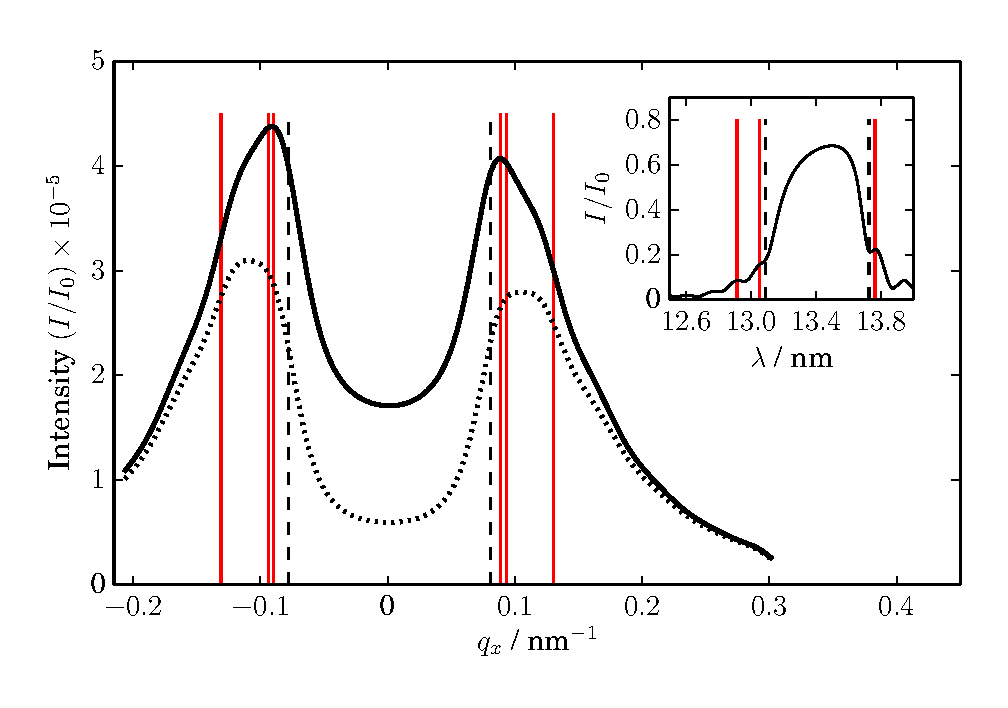
\includegraphics[width=\textwidth]{img/qx_kinematic_vs_dynamic}
        \caption{Scattering intensity distribution at $q_z=0.93$ nm$^{-1}$. The solid line shows the result of the dynamic calculation for a rocking scan with an opening angle of $\Delta\Theta=30^\circ$. The dashed line represents the calculation applying the semi-kinematic approximation, ignoring any multiple reflections within the multilayer. The dashed vertical lines are the limits of the main Bragg peak, while the red solid vertical lines show the position of dynamic contributions of the Kiessig fringes close to the main maximum. Each Kiessig fringe marked in the inset appears for the corresponding positive and negative $q_x$ value. The strong intensity at $q_x\approx0.1$ nm$^{-1}$ results from the overlap of the dynamic maxima of two different Kiessig fringes (see text).} \label{fig:kiessig_like_peak} 
\end{figure*}
The solid line corresponds to the dynamic theory, while the dotted line is the result of the semi-kinematic calculation. The dashed vertical lines indicate the limits of the main Bragg peak. These positions are defined through the first minimum on each side of the reflectivity peak (cf.~inset in Fig.~\ref{fig:kiessig_like_peak}). The vertical red lines show the position of multiple reflections due to Kiessig fringes close to the main resonance. Again, the corresponding positions in the specular reflectivity measurement are shown in the inset. Each of the marked fringes appears on the negative and positive $q_x$-axis in the main plot. This is caused by the incidence and exit angle, respectively, being at the resonance angle of the various Kiessig maxima in the reflectivity curve. Thus, a strong increase with respect to the semi-kinematic approximation is observed. The position of the dynamic contribution from the first 
Kiessig fringes on either side of the main resonance exhibits a pronounced maximum in the diffuse scattering. These fringes contribute most due to their high overall relative 
intensity compared with the fringes further away from the reflectivity maximum. In addition, the position in reciprocal space coincides with the first two Kiessig fringes marked on either side of the main maximum. This effect of dynamic maxima is similar to the observation of Bragg-like peaks in grazing incidence geometry \cite{kaganer_bragg_1995}, but it is caused by the subsidiary maxima instead. Consequently, we name this enhancement ``Kiessig-like peaks''. The contribution by the main Bragg resonance similar to the observations in Fig.~\ref{fig:Comparison_full_semi} amounts to approximately 100\% at $q_x=0$.


\subsection{Reconstruction of the PSD and the Multilayer Enhancement Factor}
\label{sec:multilayer_contribution}
The total contribution of the multilayer to the diffuse scattering, independent of lateral interface roughness properties, is described by the sum in the square brackets of Eq.~\eqref{eqn:multilayer_enhancement_factor} as a prefactor to the power spectral density $C(q_x)$. It describes the modulation of the scattering intensity due to the multilayer nature of the scattering structure, independent of the interface roughness. We thus consider it as a ``relative multilayer enhancement factor''. The result of the calculations based on the layer model of our multilayer sample is shown in Fig.~\ref{fig:MultilayerInfluence} for one detector and two rocking scan configurations. The vertical correlation length for this specific multilayer mirror is $\xi_\perp(q_x)=7.5/q_x^2$ nm$^{-1}$ as expected for a high-reflectance mirror, where $\xi_\perp$ 
exceeds the total thickness $D$ of the entire stack for $|q_x| < 0.12$ nm$^{-1}$. The method for the extraction of the vertical correlation length from the measured data is discussed in Sec.~\ref{sec:determination_of_the_psd}. The multilayer enhancement factor was normalized with respect to $q_x=0$, i.e. the calculated diffuse scattering contribution on the specular axis. 
\begin{figure}[htbp]
	\includegraphics{img/PTB17_multilayer_enhancement_factor} \caption{Enhancement factor due to the specific properties of multilayer reflectivity for three different measurement geometries. The simulations shown here were normalized with respect to the diffuse contribution to the specular reflectivity at $q_x=0$.} \label{fig:MultilayerInfluence} 
\end{figure}

The results clearly show that diffuse scattering from multilayers at near-normal incidence exhibit strong enhancement due to the intrinsically limited bandpass of reflectivity of multilayers. If both the incidence and exit angle is out of the Bragg resonance, the higher penetration depth of the multilayer causes an increase in the number of interfaces contributing to the diffuse scattering intensity. Thus higher total scattering is observed. The Kiessig fringes cause modulations in the enhancement factor increased by the purely dynamic processes described in Sec.~\ref{sec:dynamic_contributions}.

\begin{figure*}[htbp]
        \includegraphics[width=
        \textwidth]{img/PTB17_diffuse_simulation_vs_measurement} \caption{Measured (a) and simulated (b) reciprocal space maps for a rocking scan at an opening angle of $\Delta\Theta=30^\circ$ with the roughness parameters determined in Sec.~\ref{sec:determination_of_the_psd}.} \label{fig:comparisonWithTheory} 
\end{figure*}

\subsubsection{Reconstruction of the Power Spectral Density} \label{sec:determination_of_the_psd} In order to extract roughness properties from the off-specular measurements shown above, a correction for the influence of the multilayer as discussed in Sec.~\ref{sec:multilayer_contribution} is required. The scattering intensity after division by the multilayer enhancement factor represents the power spectral density of roughness. The measured PSDs are shown in Fig.~\ref{fig:PSDs_linear} for all three experiments. The excellent agreement with each other within the uncertainty margin confirms the validity and necessity of the dynamic theory to model the diffuse scattering from the multilayer. The reconstruction of the parameters of the power spectral density in Eq.~\eqref{eqn:psd} can be done by considering the overall intensity as well as the asymptotic behavior \cite{salditt_interfacial_1996} of the measured data in Fig.~\ref{fig:PSDs_linear}.

The numerical simulations show a strong sensitivity with respect to the mean roughness parameter $\sigma$ through the total portion of diffusely scattered light. As expected for a high-reflectance mirror, we obtained a small roughness value of $\sigma = 0.2$ nm.
\begin{figure}[htbp]
	\includegraphics{img/PTB17_PSD_for_all_geometries} \caption{Diffuse scattering intensity corrected for the multilayer enhancement factor considering a tilt angle of $\beta=-1^{\circ}$ according to Eq.~\eqref{eqn:tilt_correction}. The black solid line corresponds to a power spectral density with $\xi_\parallel=5.6$ nm, $H=1.0$, $\sigma=0.2$ nm and a vertical correlation length of $\xi_\perp(q_x)=7.5/q_x^2$ nm$^{-1}$.} \label{fig:PSDs_linear} 
\end{figure}

It follows from the definition of the PSD in Eq.~\eqref{eqn:psd} that the lateral correlation length $\xi_\parallel$ defines a cut-off for the spatial frequencies contributing to the off-specular scattering. We performed several simulations to compare the simulated intensity profile with the cut-off frequency observed in the measured data. A correlation length of $\xi_\parallel=5.6$ nm was obtained following this method. The fractal nature of the interfaces was analyzed by varying the Hurst parameter $H$. The asymptotic behavior of the power spectral density for $q_x>10^{-1}$~nm$^{-1}$ for the multilayer sample measured yields a Hurst factor of $H=1.0$, which corresponds to a smooth roughness profile \cite{sinha_x-ray_1988}. By following this procedure, measurements of power spectral densities are possible, independent of the measurement geometry.

For a full characterization of the multilayer, the determination of the vertical correlation length remains. This parameter is also accessible through the two-dimensional reciprocal space maps. It has been observed elsewhere that the vertical correlation of the interfacial roughness leads to resonant diffuse scattering (``Bragg sheets'')~\cite{holy_nonspecular_1994}. The width of these sheets with respect to the $q_z$-axis provides a measure for the vertical correlation lengths, e.g.~in GISAXS \cite{siffalovic_characterization_2009}. We observe a similar dependence of the scattering intensity close to the Bragg resonance along the vertical axis (cf.~Fig.~\ref{fig:Comparison_full_semi}) with a reduction of the scattering intensity at the resonance for small correlation length but a higher relative scattering intensity far off resonance (cf. $q_z>0.95$ nm$^{-1}$ in Fig.~\ref{fig:Comparison_full_semi}). We varied the vertical correlation length $\xi_\perp(q_x)$ and fitted several vertical cuts of the reciprocal space map simultaneously with the PSD determination. The best model for our sample yields a high vertical correlation length of $\xi_\perp(q_x)=7.5/q_x^2$ nm$^{-1}$, as expected for high-reflectance mirrors, at a tilt angle of $\beta=-1^\circ$ of the Bragg plane. 
This correlation length exceeds the total thickness of the multilayer coating up to $|q_x|<0.13$ nm$^{-1}$ and thus indicates (almost) full replication of roughness throughout all interfaces for the specified spacial frequencies.

By combining the findings for the properties of roughness in the power spectral density and the multilayer enhancement factor determined by the layer structure of the multilayer, we are able to fully reconstruct the measured intensity distribution for all geometries. The simulated reciprocal space map for a rocking scan with an opening angle of $\Delta\Theta = 30^\circ$ based on the parameters determined in the previous analysis is shown in Fig.~\ref{fig:comparisonWithTheory}(b). The calculation is in excellent agreement with the measured reciprocal space map in Fig.~\ref{fig:comparisonWithTheory}(a). 


\section{Roughness for Varying Mo Thickness in Mo/Si Multilayer Samples} \label{ch_diff:sec_mo_si_c}

Based on the presumed crystallization threshold found from the analysis of the specular reflectance curves, diffuse scattering measurements for selected samples from both sets were performed. In both cases, scattering maps were taken from the samples with lowest and highest Mo layer thickness, respectively, in addition to the samples with Mo thicknesses right before, at and right after the presumed crystallization threshold was investigated (cf.~marked points in Fig.~\ref{fig:fitted_mo_and_fitted_D}). The diffuse scattering was measured by keeping the detector angle with respect to the incoming beam fixed at $\Delta\Theta = 30^\circ$, while the sample was tilted from an AOI of $\alpha_i=15^\circ$ to $\alpha_i=38^\circ$ with a step size $\Delta\alpha_i = 0.5^\circ$. At each angular position, a wavelength scan from $\lambda=12.35$ nm to $\lambda=14.0$ nm in steps of $\Delta\lambda = 0.01$ nm was performed to map the diffuse scattering distribution. The results are shown in a reciprocal space representation for both sets in comparison in Fig.~\ref{fig:diffuse}.
\begin{figure*}[htbp]
\centering
\includegraphics[width=\textwidth]{img/MoSiC_diffuse_measurements}
\caption{Measured diffuse scattering distributions in reciprocal space representation shown on linear false-color scale. The selected unpolished samples are shown in a) with increasing Mo layer thickness $d_{Mo}$. The selected samples for the polished set are shown in b) also in order of increasing Mo thickness $d_{Mo}$. The samples with strongest scattering are shown in larger detail in Fig.~\ref{fig:dwba_data_best_model_comparison}.}
\label{fig:diffuse}
\end{figure*}
The maps in Fig.~\ref{fig:diffuse}a show the scattering distribution from the unpolished samples marked with the fitted Mo layer thickness (cf.~Fig.~\ref{fig:fitted_mo_and_fitted_D}). The polished samples are shown in Fig.~\ref{fig:diffuse}b. One sample in each series shows significantly stronger scattering than the others. Both sets show distinctly different scattering distributions. In both cases, the structure visible in the map is dominated by the multilayer-enhancement factor including resonant dynamic enhancement ("Kiessig-like peaks")\cite{haase_role_2014}. For the unpolished samples a downward tilted Bragg sheet can be observed. This is due to a non-orthogonal roughness correlation throughout the stack with respect to the surface \cite{gullikson_asymmetric_1999}. In the case of the polished samples, significantly less scattering can be observed for higher spatial frequencies, whereas more intensity is measured for smaller frequencies.


\subsection{Tilted Bragg Sheets}
\begin{figure*}[htbp]
\centering
\includegraphics[width=\textwidth]{img/MoSiC_diffuse_tilt_vs_notilt}
\caption{Direct comparison of the measured reciprocal space maps with the DWBA calculation resulting from the parameters obtained with the MCMC optimization procedure (see text). a) shows the maps of the unpolished sample with strongest diffuse scattering. Similarly, b) shows the maps of the polished sample at the respective presumed crystallization threshold with strongest scattering.}
\label{fig:dwba_data_best_model_comparison}
\end{figure*}
\subsection{Reconstruction of the Power Spectral Density}
The theoretical analysis was performed based on the DWBA for all scattering maps measured above. The ideal model for each sample system entering the DWBA calculation was obtained from the analysis in Sec.~\ref{sec:mo_si_model_reconstruction_results}. The optimization functional was calculated according to Eq.~\eqref{eqn:reduced_chi_2} for all off-specular wavelength scans for each angle. The combined likelihood was then calculated similarly to Eq.~\eqref{eqn:total_chi_2_diffuse}, as the sum of all measurement points for all angular positions and wavelengths. The optimization was conducted by the MCMC analysis with respect to the vertical correlation length $\xi_\perp$ in the vertical correlation function $c(q_\parallel)$ and all PSD parameters in $C(q_\parallel)$. The list of the corresponding parameters and their bounds is given in Table~\ref{tbl:diffuse_parameters}.
\begin{table*}
\centering
\caption{Parameters of the DWBA analysis with parameter limits}
\label{tbl:diffuse_parameters}
\begin{tabularx}{\textwidth}{@{}lXll@{}}
\toprule
Parameter & Definition & Lower bound & Upper bound\\ \midrule
$\sigma_r$ / nm & root mean square roughness & $0.0$& $1.0$\\ 
$\xi_\parallel$ / nm & lateral correlation length & $0.0$& $20.0$\\ 
$\xi_\perp$ / nm$^{-1}$ &vertical correlation parameter yielding vertical correlation length trough $\xi_\perp(q_\parallel) = \xi_\perp/q_\parallel^2$ &$0.0$ & $20.0$\\
$\beta$ / $^\circ$&angle for off-axis vertical roughness correlation& $-10.0$ & $10.0$\\ 
 \bottomrule
\end{tabularx}
\end{table*}

For this analysis we assumed a Gaussian roughness profile at the interfaces, which is described mathematically by setting $H\equiv1.0$ for all samples. For the two samples, the full maps with the strongest scattering from each set are shown in comparison to the best model DWBA calculation (Fig~\ref{fig:dwba_data_best_model_comparison}). The results for the roughness of the MCMC analysis are shown in Fig.~\ref{fig:PSD_results}. All values are compiled in Table~\ref{tbl:diffuse_parameters_results}. 
\begin{figure*}[htbp]
\centering
\includegraphics[width=\textwidth]{img/MoSiC_dwba_data_best_model_comparison}
\caption{Direct comparison of the measured reciprocal space maps with the DWBA calculation resulting from the parameters obtained with the MCMC optimization procedure (see text). a) shows the maps of the unpolished sample with strongest diffuse scattering. Similarly, b) shows the maps of the polished sample at the respective presumed crystallization threshold with strongest scattering.}
\label{fig:dwba_data_best_model_comparison}
\end{figure*}
\begin{figure}[htbp]
\centering
\includegraphics[width=0.7\textwidth]{img/MoSiC_PSD_results}
\caption{a) Root mean square roughness results from the analysis of the diffuse scattering for the two sample sets. In each set, an increase of roughness is observed at the crystallization threshold. For comparison, the max peak reflectance (cf.~Fig.~\ref{fig:EUV_reflectivity}c) for each sample set is shown in b). The increase in roughness clearly correlates with a significant dip in the peak reflectance as indicated by the dashed vertical lines.}
\label{fig:PSD_results}
\end{figure}
For both sample sets a significant increase of roughness can be observed at the crystallization threshold, which coincides with the lowest reflectance for that sample in each set. Interestingly, the roughness returns to the previous value for further increasing Mo layer thicknesses. The roughening due to the formation of nanocrystallites at the threshold is compensated for even larger thicknesses.
That indicates a smoothing effect due to additional Mo deposition above the crystallization threshold. We also observe a restored peak reflectance in that case. For the polished samples, the formation of crystallites can be observed with similar effects, but at lower Mo layer thickness with overall significantly lower root mean square roughness values.

\begin{table*}[htbp]
\centering
\caption{Results for the DWBA model parameters}
\label{tbl:diffuse_parameters_results}
\begin{tabular}{@{}lllll@{}}
\toprule
nom. Mo thickness / nm&$\sigma_r$ / nm & $\xi_\parallel$ / nm & $\xi_\perp$  / nm$^{-1}$ & $\beta$ / $^\circ$ \\ 
(fitted Mo thickness / nm) & & & &\\ \midrule
\multicolumn{5}{c}{Unpolished samples}\\
\midrule
$1.70$ ($1.81 \pm 0.18$) & $0.227 \pm 0.007$ & $3.14 \pm 0.11$ & $3.69 \pm 0.31$ & $-4.62 \pm 0.11$ \\
$2.21$ ($2.31 \pm 0.22$)& $0.232 \pm 0.005$ & $3.72 \pm 0.09$ & $4.88 \pm 0.35$ & $-5.02 \pm 0.09$ \\
$2.38$ ($2.43 \pm 0.12$) & $0.329 \pm 0.006$ & $4.51 \pm 0.10$ & $4.44 \pm 0.34$ & $-5.67 \pm 0.10$ \\
verification rot.~$90^\circ$ & $0.317 \pm 0.009$ & $4.56 \pm 0.18$ & $3.62 \pm 0.37$ & $+0.55 \pm 0.14$ \\
$2.54$ ($2.68 \pm 0.14$)& $0.211 \pm 0.006$ & $3.61 \pm 0.12$ & $3.80 \pm 0.31$ & $-5.06 \pm 0.12$ \\
$3.05$ ($3.22 \pm 0.12$)& $0.243 \pm 0.005$ & $2.89 \pm 0.06$ & $5.72 \pm 0.31$ & $-5.06 \pm 0.06$ \\
\midrule
\multicolumn{5}{c}{Polished samples}\\
\midrule
$1.70$ ($1.77 \pm 0.20$) & $0.129 \pm 0.006$ & $7.05 \pm 0.38$ & $0.53 \pm 0.05$ & $-1.19 \pm 0.56$ \\
$1.85$ ($1.91 \pm 0.14$)& $0.195 \pm 0.005$ & $10.66 \pm 0.34$ & $0.76 \pm 0.07$ & $-1.50 \pm 0.51$ \\
$2.00$ ($2.30 \pm 0.20$)& $0.105 \pm 0.002$ & $8.95 \pm 0.25$ & $0.76 \pm 0.06$ & $-2.28 \pm 0.30$ \\
$2.30$ ($2.59 \pm 0.13$)& $0.106 \pm 0.003$ & $8.22 \pm 0.29$ & $0.86 \pm 0.08$ & $-2.90 \pm 0.23$ \\
$3.05$ ($3.47 \pm 0.16$)& $0.088 \pm 0.002$ & $10.29 \pm 0.37$ & $1.47 \pm 0.23$ & $-1.62 \pm 0.32$ \\
 \bottomrule
\end{tabular}
\end{table*}

In addition, a large gap between the vertical correlation factors can be observed for comparing the polished and unpolished samples. As is to be expected, the polishing process largely reduces the roughness correlation between different interfaces. In the case of unpolished growth, almost the entire stack is correlated for the observable spatial frequencies. The large values for the in-planar correlation length for the polished samples are also a direct result of the polishing process. 


\section{Resolving the Roughness Correlation in Cr/Sc Multilayer Samples} \label{ch_diff:sec_CrSc}
Even in the case of the data, methods and model presented here, the combined 
analysis leaves a correlation between the intermixing parameter $\eta$ and the 
roughness $\sigma_r$, which could not be resolved (see 
Fig.~\ref{fig:eta_sigma_correlation}).
\begin{figure}[htbp]
  \centering
  \includegraphics[width=0.5\textwidth]{images/eta_sigma_correlation}
  \caption{Correlation of the projected $\chi^2$ surface onto the parameter 
pair $(\eta, \sigma_r$) by visualization of the position of the MCMC samples in 
the reduced parameter space. The strong correlation of both parameters in the 
optimal solution, which is indicated by blue solid lines, is clearly visible. 
The percentiles corresponding to one and two standard deviations $\sigma$ are 
indicated by the black contour lines.}
  \label{fig:eta_sigma_correlation}
\end{figure}
This means that none of the methods, not even the combined analysis, contains 
sufficient information to deduct an unambiguous result for the roughness or 
intermixing. Intermixing alone merely reduces optical contrast, whereas 
interface roughness causes diffuse scattering. One should be able to 
distinguish between the two through the measurement of the diffuse scattering. 
The distribution of the off-specular scattering with respect to the scattering 
angle and wavelength provides additional information on the vertical and 
lateral correlation of spatial roughness frequencies. The latter is described 
by the power spectral density. We conducted a diffuse scattering experiment as 
described in Sec.~\ref{sec:experimental}. The analysis was conducted based on 
the DWBA formalism outlined in Sec.~\ref{sec:matrix_formalism}. The subfigures 
(a) and (b) of Fig.~\ref{fig:diffuse_meas} show the measured reciprocal space 
map in direct comparison to the best model found within the DWBA approach.
\onecolumn
\begin{figure}[htbp]
  \centering
  \includegraphics[width=0.7\textwidth]{img/CrSc_diffuse_measured_vs_dwba}
  \caption{a) Diffuse scattering measurement in $q$-space representation and 
log scale. b) DWBA calculation of the optimal PSD model based on the electron 
density profile with the multilayer parameters for the combined analysis listed 
in Table~\ref{tbl:results}.}
  \label{fig:diffuse_meas}
\end{figure}

\begin{figure}[htbp]
  \centering
  \includegraphics[width=0.7\textwidth]{img/CrSc_diffuse_vertical_correlation}
  \caption{ Vertical cut at the indicated white dashed cut 
positions in (a) and (b). The blue dashed lines show two limiting cases for the 
value of the vertical correlation length. The result is a model uncertainty in 
the PSD.}
  \label{fig:diffuse_meas}
\end{figure}

\begin{figure}[htbp]
  \centering
  \includegraphics[width=0.7\textwidth]{img/CrSc_diffuse_PSD}
  \caption{Comparison of the extracted effective PSDs from the diffuse 
scattering measurement (Measured Data) shown in (a) and the DWBA calculation of 
(b) at the horizontal cut positions indicated by the white dashed lines. The 
uncertainty interval for the extracted power spectral density is shown by the 
two dashed PSD profiles (see main text).}
  \label{fig:diffuse_meas}
\end{figure}


The formation of a narrow Bragg sheet \cite{haase_role_2014,salditt_kinetic_1994} 
confirms the high degree of roughness correlation and thereby justifies the 
approximations made in Sec.~\ref{sec:matrix_formalism} for identical roughness 
properties at each interface. To deduct the effective power spectral density 
shown in Fig.~\ref{fig:diffuse_meas}(c), we have taken a cut along the Bragg 
sheet as indicated by the horizontal white dashed lines in the reciprocal space 
maps. We divided the extracted scattering intensity by the multilayer 
enhancement factor in Eq.~\ref{eqn:dwba}, leaving the contribution of the 
effective PSD $C(q_\parallel)$ to the diffuse scattering.
This requires that the vertical correlation factor $\xi_\perp$ be determined 
first, which enters the calculation of the multilayer enhancement factor 
through the replication factor in Eq.~\eqref{eqn:vertical_correlation}. Due to 
the very high computational cost of a MCMC procedure, we have instead 
calculated two limiting cases of the vertical correlation. This was done by 
analyzing the width of the Bragg sheet at the vertical white dashed cut 
positions, indicated in Fig.~\ref{fig:diffuse_meas}(a,b), and comparing the 
simulated intensity distribution with the measurement uncertainty. The two 
limiting cases are shown in Fig.~\ref{fig:diffuse_meas}(d) (blue dashed curves) 
including the best model (solid blue curve) in comparison with the measured 
data (solid red curve). Proceeding from here, we have evaluated the measured 
PSD with the corresponding multilayer enhancement factor as described above. 
Again, the two limiting cases are shown as red dashed curves in 
Fig.~\ref{fig:diffuse_meas}(c) including the PSD deduced from the best model 
value for $\xi_\perp$ as a solid red curve. The root mean square (r.m.s.) 
roughness deducted from these PSDs is given by the two-dimensional integral as
\begin{align}
\sigma_r &=\frac{1}{2\pi} \sqrt{\int_{0}^{\infty} q_\parallel C(q_\parallel) \, 
dq_\parallel} \text{.}
\end{align}
The uncertainty of the PSD due to the vertical correlation leads to an 
uncertainty in the r.m.s. roughness when evaluating the integral. Due to the 
limited $q_\parallel$ range where measurements can be taken, we have fitted the 
PSD model of Eq.~\eqref{eqn:psd} to the three resulting PSDs and performed the 
integration over the full $q_\parallel$ range. The deviation of the integration 
for the PSD model fit and the data in the available range were negligible. The 
best model results for the vertical replication factor and the power spectral 
density are given in Table.~\ref{tbl:psd_results}, together with their 
uncertainties resulting from the described procedure. The best fit of the PSD 
model is shown in Fig.~\ref{fig:diffuse_meas}(c) as a solid blue curve.
\begin{table}
\centering
\caption{Best model parameters of the PSD as a result of the diffuse scattering 
analysis}
\label{tbl:psd_results}
\begin{tabular}{@{}ll@{}}
\toprule
Parameter & Best model values\\ \midrule
$\sigma_r$ / nm & $0.17 \pm 0.02$ \\
$\xi_\parallel$ / nm& $4.00 \pm 0.35$ \\
$\xi_\perp$  / nm$^{-1}$& $10.5 \pm 3.5$ \\
$H$ & $1.0$ \\
$\beta$ & $0.0$ \\
 \bottomrule
\end{tabular}
\end{table}
The r.m.s.~roughness value found with the analysis of the diffuse scattering is 
identical within its uncertainty interval to the value obtained from the 
combined analysis and thus confirms the intermixing and roughness parameters 
listed in Table.~\ref{tbl:results}.

    %\chapter{Summary and Outlook} \label{ch_summary}


    \printbibliography[heading=bibintoc,title={References}]


\backmatter
    \pagestyle{thesisINTRO}
    %\pagestyle{empty}
\selectlanguage{ngerman}
\noindent
\section*{Acknowledgement}
At this point, I would like to express my gratitude to all of those who directly or indirectly contributed to the successful completion of this thesis.

First and foremost, I would like to thank Dr.~Frank Scholze, head of the EUV radiometry group at the Physikalisch-Technische Bundesanstalt, for giving me the chance to conduct the work leading to this PhD thesis under his supervision. Our numerous scientific discussions, his valuable ideas and his constructive criticism bundled with the opportunity to conduct experiments even on a short notice, contributed significantly to the success of this thesis. His encouragement and support to present my results to an international scientific audience allowed me to establish contacts and to shape my professional future.

Furthermore, I would like to thank Prof.~Dr.~Mathias Richter for his support and the examination of this thesis. He always had an open ear and valuable advise for the course of my scientific work and the near future. 

I am very grateful to Prof.~Dr.~Stefan Eisebitt for supporting and evaluating my dissertation and to Dr.~Sa\v{s}a Bajt for the fruitful discussions, for providing me with the Cr/Sc samples for my experiments and her willingness to serve as evaluator of this thesis. 




\cleardoublepage

    %\include{tub-eidesstattliche}
    %% publication list
\noindent
\pagestyle{empty}
\selectlanguage{ngerman}

\section*{Erklärung}

Es wurden bereits Teile der Dissertation veröffentlicht.
\vspace{2ex}

Liste der Veröffentlichungen, welche in die Dissertation eingeflossen sind:

\begin{enumerate}[label=\arabic*) ]
    \item \fullcite{haase_role_2014} 

    \item \fullcite{haase_characterization_2015} 

    \item \fullcite{haase_multiparameter_2016} 

    \item \fullcite{haase_interface_2017} 

\end{enumerate}
Liste der Veröffentlichungen, welche nicht in die Dissertation eingeflossen sind:
\begin{enumerate}[label=\arabic*) ]
    \item \fullcite{prasciolu_extended_2015} 

    \item \fullcite{soltwisch_correlated_2016} 
    
\end{enumerate}


Ich habe an keiner anderen Hochschule oder Fakultät eine Promotionsabsicht eingereicht.

\vspace{3cm}

\noindent Berlin, den \today \hfill Anton Haase

\cleardoublepage

    
\iffalse
    \bibliography{zotero-full.bib}
\fi

\end{document}
